% Options for packages loaded elsewhere
% Options for packages loaded elsewhere
\PassOptionsToPackage{unicode}{hyperref}
\PassOptionsToPackage{hyphens}{url}
\PassOptionsToPackage{dvipsnames,svgnames,x11names}{xcolor}
%
\documentclass[
  letterpaper,
  DIV=11,
  numbers=noendperiod]{scrartcl}
\usepackage{xcolor}
\usepackage[margin=1in]{geometry}
\usepackage{amsmath,amssymb}
\setcounter{secnumdepth}{-\maxdimen} % remove section numbering
\usepackage{iftex}
\ifPDFTeX
  \usepackage[T1]{fontenc}
  \usepackage[utf8]{inputenc}
  \usepackage{textcomp} % provide euro and other symbols
\else % if luatex or xetex
  \usepackage{unicode-math} % this also loads fontspec
  \defaultfontfeatures{Scale=MatchLowercase}
  \defaultfontfeatures[\rmfamily]{Ligatures=TeX,Scale=1}
\fi
\usepackage{lmodern}
\ifPDFTeX\else
  % xetex/luatex font selection
\fi
% Use upquote if available, for straight quotes in verbatim environments
\IfFileExists{upquote.sty}{\usepackage{upquote}}{}
\IfFileExists{microtype.sty}{% use microtype if available
  \usepackage[]{microtype}
  \UseMicrotypeSet[protrusion]{basicmath} % disable protrusion for tt fonts
}{}
\makeatletter
\@ifundefined{KOMAClassName}{% if non-KOMA class
  \IfFileExists{parskip.sty}{%
    \usepackage{parskip}
  }{% else
    \setlength{\parindent}{0pt}
    \setlength{\parskip}{6pt plus 2pt minus 1pt}}
}{% if KOMA class
  \KOMAoptions{parskip=half}}
\makeatother
% Make \paragraph and \subparagraph free-standing
\makeatletter
\ifx\paragraph\undefined\else
  \let\oldparagraph\paragraph
  \renewcommand{\paragraph}{
    \@ifstar
      \xxxParagraphStar
      \xxxParagraphNoStar
  }
  \newcommand{\xxxParagraphStar}[1]{\oldparagraph*{#1}\mbox{}}
  \newcommand{\xxxParagraphNoStar}[1]{\oldparagraph{#1}\mbox{}}
\fi
\ifx\subparagraph\undefined\else
  \let\oldsubparagraph\subparagraph
  \renewcommand{\subparagraph}{
    \@ifstar
      \xxxSubParagraphStar
      \xxxSubParagraphNoStar
  }
  \newcommand{\xxxSubParagraphStar}[1]{\oldsubparagraph*{#1}\mbox{}}
  \newcommand{\xxxSubParagraphNoStar}[1]{\oldsubparagraph{#1}\mbox{}}
\fi
\makeatother

\usepackage{color}
\usepackage{fancyvrb}
\newcommand{\VerbBar}{|}
\newcommand{\VERB}{\Verb[commandchars=\\\{\}]}
\DefineVerbatimEnvironment{Highlighting}{Verbatim}{commandchars=\\\{\}}
% Add ',fontsize=\small' for more characters per line
\usepackage{framed}
\definecolor{shadecolor}{RGB}{241,243,245}
\newenvironment{Shaded}{\begin{snugshade}}{\end{snugshade}}
\newcommand{\AlertTok}[1]{\textcolor[rgb]{0.68,0.00,0.00}{#1}}
\newcommand{\AnnotationTok}[1]{\textcolor[rgb]{0.37,0.37,0.37}{#1}}
\newcommand{\AttributeTok}[1]{\textcolor[rgb]{0.40,0.45,0.13}{#1}}
\newcommand{\BaseNTok}[1]{\textcolor[rgb]{0.68,0.00,0.00}{#1}}
\newcommand{\BuiltInTok}[1]{\textcolor[rgb]{0.00,0.23,0.31}{#1}}
\newcommand{\CharTok}[1]{\textcolor[rgb]{0.13,0.47,0.30}{#1}}
\newcommand{\CommentTok}[1]{\textcolor[rgb]{0.37,0.37,0.37}{#1}}
\newcommand{\CommentVarTok}[1]{\textcolor[rgb]{0.37,0.37,0.37}{\textit{#1}}}
\newcommand{\ConstantTok}[1]{\textcolor[rgb]{0.56,0.35,0.01}{#1}}
\newcommand{\ControlFlowTok}[1]{\textcolor[rgb]{0.00,0.23,0.31}{\textbf{#1}}}
\newcommand{\DataTypeTok}[1]{\textcolor[rgb]{0.68,0.00,0.00}{#1}}
\newcommand{\DecValTok}[1]{\textcolor[rgb]{0.68,0.00,0.00}{#1}}
\newcommand{\DocumentationTok}[1]{\textcolor[rgb]{0.37,0.37,0.37}{\textit{#1}}}
\newcommand{\ErrorTok}[1]{\textcolor[rgb]{0.68,0.00,0.00}{#1}}
\newcommand{\ExtensionTok}[1]{\textcolor[rgb]{0.00,0.23,0.31}{#1}}
\newcommand{\FloatTok}[1]{\textcolor[rgb]{0.68,0.00,0.00}{#1}}
\newcommand{\FunctionTok}[1]{\textcolor[rgb]{0.28,0.35,0.67}{#1}}
\newcommand{\ImportTok}[1]{\textcolor[rgb]{0.00,0.46,0.62}{#1}}
\newcommand{\InformationTok}[1]{\textcolor[rgb]{0.37,0.37,0.37}{#1}}
\newcommand{\KeywordTok}[1]{\textcolor[rgb]{0.00,0.23,0.31}{\textbf{#1}}}
\newcommand{\NormalTok}[1]{\textcolor[rgb]{0.00,0.23,0.31}{#1}}
\newcommand{\OperatorTok}[1]{\textcolor[rgb]{0.37,0.37,0.37}{#1}}
\newcommand{\OtherTok}[1]{\textcolor[rgb]{0.00,0.23,0.31}{#1}}
\newcommand{\PreprocessorTok}[1]{\textcolor[rgb]{0.68,0.00,0.00}{#1}}
\newcommand{\RegionMarkerTok}[1]{\textcolor[rgb]{0.00,0.23,0.31}{#1}}
\newcommand{\SpecialCharTok}[1]{\textcolor[rgb]{0.37,0.37,0.37}{#1}}
\newcommand{\SpecialStringTok}[1]{\textcolor[rgb]{0.13,0.47,0.30}{#1}}
\newcommand{\StringTok}[1]{\textcolor[rgb]{0.13,0.47,0.30}{#1}}
\newcommand{\VariableTok}[1]{\textcolor[rgb]{0.07,0.07,0.07}{#1}}
\newcommand{\VerbatimStringTok}[1]{\textcolor[rgb]{0.13,0.47,0.30}{#1}}
\newcommand{\WarningTok}[1]{\textcolor[rgb]{0.37,0.37,0.37}{\textit{#1}}}

\usepackage{longtable,booktabs,array}
\newcounter{none} % for unnumbered tables
\usepackage{calc} % for calculating minipage widths
% Correct order of tables after \paragraph or \subparagraph
\usepackage{etoolbox}
\makeatletter
\patchcmd\longtable{\par}{\if@noskipsec\mbox{}\fi\par}{}{}
\makeatother
% Allow footnotes in longtable head/foot
\IfFileExists{footnotehyper.sty}{\usepackage{footnotehyper}}{\usepackage{footnote}}
\makesavenoteenv{longtable}
\usepackage{graphicx}
\makeatletter
\newsavebox\pandoc@box
\newcommand*\pandocbounded[1]{% scales image to fit in text height/width
  \sbox\pandoc@box{#1}%
  \Gscale@div\@tempa{\textheight}{\dimexpr\ht\pandoc@box+\dp\pandoc@box\relax}%
  \Gscale@div\@tempb{\linewidth}{\wd\pandoc@box}%
  \ifdim\@tempb\p@<\@tempa\p@\let\@tempa\@tempb\fi% select the smaller of both
  \ifdim\@tempa\p@<\p@\scalebox{\@tempa}{\usebox\pandoc@box}%
  \else\usebox{\pandoc@box}%
  \fi%
}
% Set default figure placement to htbp
\def\fps@figure{htbp}
\makeatother





\setlength{\emergencystretch}{3em} % prevent overfull lines

\providecommand{\tightlist}{%
  \setlength{\itemsep}{0pt}\setlength{\parskip}{0pt}}



 


\usepackage{amsmath,amssymb}
\KOMAoption{captions}{tableheading}
\makeatletter
\@ifpackageloaded{caption}{}{\usepackage{caption}}
\AtBeginDocument{%
\ifdefined\contentsname
  \renewcommand*\contentsname{Table of contents}
\else
  \newcommand\contentsname{Table of contents}
\fi
\ifdefined\listfigurename
  \renewcommand*\listfigurename{List of Figures}
\else
  \newcommand\listfigurename{List of Figures}
\fi
\ifdefined\listtablename
  \renewcommand*\listtablename{List of Tables}
\else
  \newcommand\listtablename{List of Tables}
\fi
\ifdefined\figurename
  \renewcommand*\figurename{Figure}
\else
  \newcommand\figurename{Figure}
\fi
\ifdefined\tablename
  \renewcommand*\tablename{Table}
\else
  \newcommand\tablename{Table}
\fi
}
\@ifpackageloaded{float}{}{\usepackage{float}}
\floatstyle{ruled}
\@ifundefined{c@chapter}{\newfloat{codelisting}{h}{lop}}{\newfloat{codelisting}{h}{lop}[chapter]}
\floatname{codelisting}{Listing}
\newcommand*\listoflistings{\listof{codelisting}{List of Listings}}
\makeatother
\makeatletter
\makeatother
\makeatletter
\@ifpackageloaded{caption}{}{\usepackage{caption}}
\@ifpackageloaded{subcaption}{}{\usepackage{subcaption}}
\makeatother
\usepackage{bookmark}
\IfFileExists{xurl.sty}{\usepackage{xurl}}{} % add URL line breaks if available
\urlstyle{same}
\hypersetup{
  pdftitle={STAT 238 --- Homework Five},
  pdfauthor={Thomas Lee},
  colorlinks=true,
  linkcolor={blue},
  filecolor={Maroon},
  citecolor={Blue},
  urlcolor={Blue},
  pdfcreator={LaTeX via pandoc}}


\title{STAT 238 --- Homework Five}
\author{Thomas Lee}
\date{2026-01-01}
\begin{document}
\maketitle


\section{Setup}\label{setup}

\begin{Shaded}
\begin{Highlighting}[]
\ImportTok{import}\NormalTok{ numpy }\ImportTok{as}\NormalTok{ np}
\ImportTok{import}\NormalTok{ pandas }\ImportTok{as}\NormalTok{ pd}
\ImportTok{import}\NormalTok{ matplotlib.pyplot }\ImportTok{as}\NormalTok{ plt}
\ImportTok{from}\NormalTok{ scipy.stats }\ImportTok{import}\NormalTok{ norm, chi2, gamma }\ImportTok{as}\NormalTok{ sp\_gamma}
\ImportTok{from}\NormalTok{ scipy.linalg }\ImportTok{import}\NormalTok{ solve, solve\_triangular}
\ImportTok{from}\NormalTok{ scipy.linalg }\ImportTok{import}\NormalTok{ svd }\ImportTok{as}\NormalTok{ lsvd}
\ImportTok{from}\NormalTok{ scipy.special }\ImportTok{import}\NormalTok{ gammaln}
\ImportTok{from}\NormalTok{ scipy.optimize }\ImportTok{import}\NormalTok{ minimize}
\ImportTok{import}\NormalTok{ statsmodels.api }\ImportTok{as}\NormalTok{ sm}
\ImportTok{import}\NormalTok{ pymc }\ImportTok{as}\NormalTok{ pm}
\ImportTok{import}\NormalTok{ arviz }\ImportTok{as}\NormalTok{ az}
\ImportTok{import}\NormalTok{ pytensor.tensor }\ImportTok{as}\NormalTok{ pt}
\ImportTok{import}\NormalTok{ warnings}
\NormalTok{warnings.filterwarnings(}\StringTok{\textquotesingle{}ignore\textquotesingle{}}\NormalTok{)}
\end{Highlighting}
\end{Shaded}

\begin{Shaded}
\begin{Highlighting}[]
\CommentTok{\# Shared utilities (from SKILL.md)}
\KeywordTok{def}\NormalTok{ mh\_sampler(log\_post\_fn, theta\_init, proposal\_sd, n\_samples}\OperatorTok{=}\DecValTok{20000}\NormalTok{, burn\_in}\OperatorTok{=}\DecValTok{5000}\NormalTok{):}
\NormalTok{    theta }\OperatorTok{=}\NormalTok{ np.atleast\_1d(np.array(theta\_init, dtype}\OperatorTok{=}\BuiltInTok{float}\NormalTok{))}
\NormalTok{    dim }\OperatorTok{=} \BuiltInTok{len}\NormalTok{(theta)}
\NormalTok{    samples }\OperatorTok{=}\NormalTok{ np.zeros((n\_samples, dim))}
\NormalTok{    log\_p\_curr }\OperatorTok{=}\NormalTok{ log\_post\_fn(theta)}
\NormalTok{    n\_accept }\OperatorTok{=} \DecValTok{0}
    \ControlFlowTok{for}\NormalTok{ i }\KeywordTok{in} \BuiltInTok{range}\NormalTok{(n\_samples):}
\NormalTok{        proposal }\OperatorTok{=}\NormalTok{ theta }\OperatorTok{+}\NormalTok{ np.random.randn(dim) }\OperatorTok{*}\NormalTok{ proposal\_sd}
\NormalTok{        log\_p\_prop }\OperatorTok{=}\NormalTok{ log\_post\_fn(proposal)}
        \ControlFlowTok{if}\NormalTok{ np.log(np.random.rand()) }\OperatorTok{\textless{}}\NormalTok{ log\_p\_prop }\OperatorTok{{-}}\NormalTok{ log\_p\_curr:}
\NormalTok{            theta }\OperatorTok{=}\NormalTok{ proposal}
\NormalTok{            log\_p\_curr }\OperatorTok{=}\NormalTok{ log\_p\_prop}
\NormalTok{            n\_accept }\OperatorTok{+=} \DecValTok{1}
\NormalTok{        samples[i] }\OperatorTok{=}\NormalTok{ theta}
    \ControlFlowTok{return}\NormalTok{ samples[burn\_in:], n\_accept }\OperatorTok{/}\NormalTok{ n\_samples}

\KeywordTok{def}\NormalTok{ mh\_sampler\_cov(log\_post\_fn, theta\_init, L\_prop, n\_samples}\OperatorTok{=}\DecValTok{25000}\NormalTok{, burn\_in}\OperatorTok{=}\DecValTok{5000}\NormalTok{):}
\NormalTok{    theta }\OperatorTok{=}\NormalTok{ np.array(theta\_init, dtype}\OperatorTok{=}\BuiltInTok{float}\NormalTok{)}
\NormalTok{    dim }\OperatorTok{=} \BuiltInTok{len}\NormalTok{(theta)}
\NormalTok{    samples }\OperatorTok{=}\NormalTok{ np.zeros((n\_samples, dim))}
\NormalTok{    log\_p\_curr }\OperatorTok{=}\NormalTok{ log\_post\_fn(theta)}
\NormalTok{    n\_accept }\OperatorTok{=} \DecValTok{0}
    \ControlFlowTok{for}\NormalTok{ i }\KeywordTok{in} \BuiltInTok{range}\NormalTok{(n\_samples):}
\NormalTok{        proposal }\OperatorTok{=}\NormalTok{ theta }\OperatorTok{+}\NormalTok{ L\_prop }\OperatorTok{@}\NormalTok{ np.random.randn(dim)}
\NormalTok{        log\_p\_prop }\OperatorTok{=}\NormalTok{ log\_post\_fn(proposal)}
        \ControlFlowTok{if}\NormalTok{ np.log(np.random.rand()) }\OperatorTok{\textless{}}\NormalTok{ log\_p\_prop }\OperatorTok{{-}}\NormalTok{ log\_p\_curr:}
\NormalTok{            theta }\OperatorTok{=}\NormalTok{ proposal}
\NormalTok{            log\_p\_curr }\OperatorTok{=}\NormalTok{ log\_p\_prop}
\NormalTok{            n\_accept }\OperatorTok{+=} \DecValTok{1}
\NormalTok{        samples[i] }\OperatorTok{=}\NormalTok{ theta}
    \ControlFlowTok{return}\NormalTok{ samples[burn\_in:], n\_accept }\OperatorTok{/}\NormalTok{ n\_samples}

\KeywordTok{def}\NormalTok{ plot\_traces(samples, param\_names, title}\OperatorTok{=}\StringTok{"Trace plots"}\NormalTok{):}
\NormalTok{    n\_params }\OperatorTok{=} \BuiltInTok{len}\NormalTok{(param\_names)}
\NormalTok{    fig, axes }\OperatorTok{=}\NormalTok{ plt.subplots(n\_params, }\DecValTok{2}\NormalTok{, figsize}\OperatorTok{=}\NormalTok{(}\DecValTok{12}\NormalTok{, }\FloatTok{2.6} \OperatorTok{*}\NormalTok{ n\_params))}
    \ControlFlowTok{if}\NormalTok{ n\_params }\OperatorTok{==} \DecValTok{1}\NormalTok{:}
\NormalTok{        axes }\OperatorTok{=}\NormalTok{ axes[}\VariableTok{None}\NormalTok{, :]}
    \ControlFlowTok{for}\NormalTok{ i, name }\KeywordTok{in} \BuiltInTok{enumerate}\NormalTok{(param\_names):}
\NormalTok{        s }\OperatorTok{=}\NormalTok{ samples[:, i]}
\NormalTok{        axes[i, }\DecValTok{0}\NormalTok{].plot(s, lw}\OperatorTok{=}\FloatTok{0.5}\NormalTok{, alpha}\OperatorTok{=}\FloatTok{0.7}\NormalTok{, color}\OperatorTok{=}\StringTok{"steelblue"}\NormalTok{)}
\NormalTok{        axes[i, }\DecValTok{0}\NormalTok{].set\_title(}\SpecialStringTok{f"Trace: }\SpecialCharTok{\{}\NormalTok{name}\SpecialCharTok{\}}\SpecialStringTok{"}\NormalTok{)}
\NormalTok{        axes[i, }\DecValTok{0}\NormalTok{].set\_xlabel(}\StringTok{"Iteration"}\NormalTok{)}
\NormalTok{        axes[i, }\DecValTok{1}\NormalTok{].hist(s, bins}\OperatorTok{=}\DecValTok{50}\NormalTok{, density}\OperatorTok{=}\VariableTok{True}\NormalTok{, color}\OperatorTok{=}\StringTok{"steelblue"}\NormalTok{, alpha}\OperatorTok{=}\FloatTok{0.7}\NormalTok{)}
\NormalTok{        axes[i, }\DecValTok{1}\NormalTok{].set\_title(}\SpecialStringTok{f"Posterior: }\SpecialCharTok{\{}\NormalTok{name}\SpecialCharTok{\}}\SpecialStringTok{"}\NormalTok{)}
\NormalTok{    plt.suptitle(title, y}\OperatorTok{=}\FloatTok{1.01}\NormalTok{)}
\NormalTok{    plt.tight\_layout()}
\NormalTok{    plt.show()}

\KeywordTok{def}\NormalTok{ print\_comparison(param\_names, methods\_dict):}
\NormalTok{    method\_names }\OperatorTok{=} \BuiltInTok{list}\NormalTok{(methods\_dict.keys())}
\NormalTok{    header }\OperatorTok{=} \SpecialStringTok{f"}\SpecialCharTok{\{}\StringTok{\textquotesingle{}Parameter\textquotesingle{}}\SpecialCharTok{:\textless{}14\}}\SpecialStringTok{"}
    \ControlFlowTok{for}\NormalTok{ m }\KeywordTok{in}\NormalTok{ method\_names:}
\NormalTok{        header }\OperatorTok{+=} \SpecialStringTok{f"  }\SpecialCharTok{\{}\NormalTok{m}\OperatorTok{+}\StringTok{\textquotesingle{} mean\textquotesingle{}}\SpecialCharTok{:\textgreater{}12\}}\SpecialStringTok{  }\SpecialCharTok{\{}\NormalTok{m}\OperatorTok{+}\StringTok{\textquotesingle{} sd\textquotesingle{}}\SpecialCharTok{:\textgreater{}10\}}\SpecialStringTok{"}
    \BuiltInTok{print}\NormalTok{(header)}
    \BuiltInTok{print}\NormalTok{(}\StringTok{"{-}"} \OperatorTok{*} \BuiltInTok{len}\NormalTok{(header))}
    \ControlFlowTok{for}\NormalTok{ i, p }\KeywordTok{in} \BuiltInTok{enumerate}\NormalTok{(param\_names):}
\NormalTok{        row }\OperatorTok{=} \SpecialStringTok{f"}\SpecialCharTok{\{}\NormalTok{p}\SpecialCharTok{:\textless{}14\}}\SpecialStringTok{"}
        \ControlFlowTok{for}\NormalTok{ means, sds }\KeywordTok{in}\NormalTok{ methods\_dict.values():}
\NormalTok{            row }\OperatorTok{+=} \SpecialStringTok{f"  }\SpecialCharTok{\{}\NormalTok{means[i]}\SpecialCharTok{:\textgreater{}12.4f\}}\SpecialStringTok{  }\SpecialCharTok{\{}\NormalTok{sds[i]}\SpecialCharTok{:\textgreater{}10.4f\}}\SpecialStringTok{"}
        \BuiltInTok{print}\NormalTok{(row)}
\end{Highlighting}
\end{Shaded}

\newpage

\section{Problem 1 --- Cauchy Location}\label{problem-1-cauchy-location}

\textbf{Model.}
\(x_i \mid \theta \overset{\text{iid}}{\sim} \text{Cauchy}(\theta, 1)\)
for \(i=1,\dots,5\), with prior \(\theta \sim \text{Unif}[0, 100]\). The
unnormalized log-posterior is \[
\log \pi(\theta \mid x) \;=\; -\sum_{i=1}^{5} \log\!\bigl(1 + (x_i - \theta)^2\bigr), \qquad \theta \in [0, 100].
\]

\begin{Shaded}
\begin{Highlighting}[]
\NormalTok{x\_obs }\OperatorTok{=}\NormalTok{ np.array([}\FloatTok{44.0}\NormalTok{, }\FloatTok{43.0}\NormalTok{, }\FloatTok{47.5}\NormalTok{, }\FloatTok{46.5}\NormalTok{, }\FloatTok{45.0}\NormalTok{])}

\KeywordTok{def}\NormalTok{ log\_post\_cauchy(theta, x\_obs}\OperatorTok{=}\NormalTok{x\_obs, lo}\OperatorTok{=}\FloatTok{0.0}\NormalTok{, hi}\OperatorTok{=}\FloatTok{100.0}\NormalTok{):}
\NormalTok{    theta }\OperatorTok{=} \BuiltInTok{float}\NormalTok{(np.asarray(theta).ravel()[}\DecValTok{0}\NormalTok{])}
    \ControlFlowTok{if} \KeywordTok{not}\NormalTok{ (lo }\OperatorTok{\textless{}}\NormalTok{ theta }\OperatorTok{\textless{}}\NormalTok{ hi):}
        \ControlFlowTok{return} \OperatorTok{{-}}\NormalTok{np.inf}
    \ControlFlowTok{return} \OperatorTok{{-}}\NormalTok{np.}\BuiltInTok{sum}\NormalTok{(np.log(}\FloatTok{1.0} \OperatorTok{+}\NormalTok{ (x\_obs }\OperatorTok{{-}}\NormalTok{ theta)}\OperatorTok{**}\DecValTok{2}\NormalTok{))}
\end{Highlighting}
\end{Shaded}

\subsection{(a) Grid posterior}\label{a-grid-posterior}

\begin{Shaded}
\begin{Highlighting}[]
\NormalTok{theta\_grid }\OperatorTok{=}\NormalTok{ np.linspace(}\FloatTok{0.001}\NormalTok{, }\FloatTok{99.999}\NormalTok{, }\DecValTok{5000}\NormalTok{)}
\NormalTok{log\_post\_vals }\OperatorTok{=}\NormalTok{ np.array([log\_post\_cauchy(t) }\ControlFlowTok{for}\NormalTok{ t }\KeywordTok{in}\NormalTok{ theta\_grid])}
\NormalTok{log\_post\_vals }\OperatorTok{{-}=}\NormalTok{ log\_post\_vals.}\BuiltInTok{max}\NormalTok{()}
\NormalTok{post\_grid }\OperatorTok{=}\NormalTok{ np.exp(log\_post\_vals)}
\NormalTok{dtheta }\OperatorTok{=}\NormalTok{ theta\_grid[}\DecValTok{1}\NormalTok{] }\OperatorTok{{-}}\NormalTok{ theta\_grid[}\DecValTok{0}\NormalTok{]}
\NormalTok{post\_grid }\OperatorTok{/=}\NormalTok{ post\_grid.}\BuiltInTok{sum}\NormalTok{() }\OperatorTok{*}\NormalTok{ dtheta}

\NormalTok{post\_mean\_grid }\OperatorTok{=}\NormalTok{ np.}\BuiltInTok{sum}\NormalTok{(theta\_grid }\OperatorTok{*}\NormalTok{ post\_grid) }\OperatorTok{*}\NormalTok{ dtheta}
\NormalTok{cdf\_grid }\OperatorTok{=}\NormalTok{ np.cumsum(post\_grid) }\OperatorTok{*}\NormalTok{ dtheta}
\NormalTok{ci\_lo }\OperatorTok{=}\NormalTok{ theta\_grid[np.searchsorted(cdf\_grid, }\FloatTok{0.025}\NormalTok{)]}
\NormalTok{ci\_hi }\OperatorTok{=}\NormalTok{ theta\_grid[np.searchsorted(cdf\_grid, }\FloatTok{0.975}\NormalTok{)]}
\BuiltInTok{print}\NormalTok{(}\SpecialStringTok{f"Grid posterior mean: }\SpecialCharTok{\{}\NormalTok{post\_mean\_grid}\SpecialCharTok{:.4f\}}\SpecialStringTok{"}\NormalTok{)}
\BuiltInTok{print}\NormalTok{(}\SpecialStringTok{f"Grid 95\% CI: [}\SpecialCharTok{\{}\NormalTok{ci\_lo}\SpecialCharTok{:.4f\}}\SpecialStringTok{, }\SpecialCharTok{\{}\NormalTok{ci\_hi}\SpecialCharTok{:.4f\}}\SpecialStringTok{]"}\NormalTok{)}

\NormalTok{plt.figure(figsize}\OperatorTok{=}\NormalTok{(}\DecValTok{8}\NormalTok{, }\DecValTok{4}\NormalTok{))}
\NormalTok{plt.plot(theta\_grid, post\_grid, color}\OperatorTok{=}\StringTok{"steelblue"}\NormalTok{, lw}\OperatorTok{=}\DecValTok{2}\NormalTok{)}
\NormalTok{plt.xlim(}\DecValTok{40}\NormalTok{, }\DecValTok{50}\NormalTok{)}
\NormalTok{plt.xlabel(}\VerbatimStringTok{r"}\DecValTok{$}\CharTok{\textbackslash{}t}\VerbatimStringTok{heta}\DecValTok{$}\VerbatimStringTok{"}\NormalTok{)}\OperatorTok{;}\NormalTok{ plt.ylabel(}\StringTok{"Posterior density"}\NormalTok{)}
\NormalTok{plt.title(}\VerbatimStringTok{r"Grid posterior of }\DecValTok{$}\CharTok{\textbackslash{}t}\VerbatimStringTok{heta}\DecValTok{$}\VerbatimStringTok{"}\NormalTok{)}
\NormalTok{plt.tight\_layout()}\OperatorTok{;}\NormalTok{ plt.show()}
\end{Highlighting}
\end{Shaded}

\begin{verbatim}
Grid posterior mean: 45.0778
Grid 95% CI: [43.2688, 47.0695]
\end{verbatim}

\pandocbounded{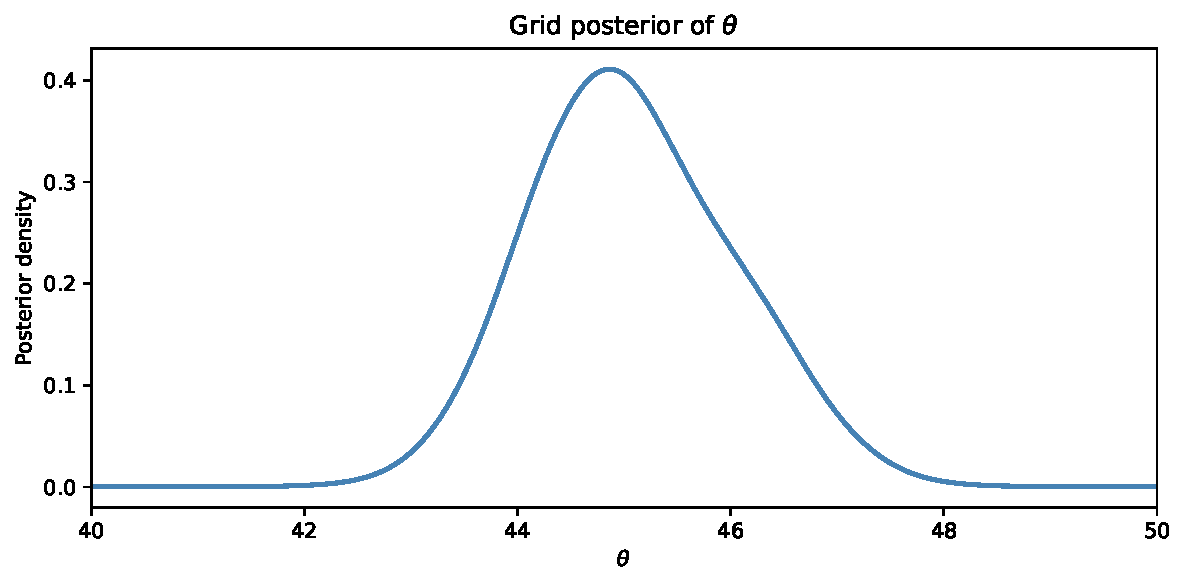
\includegraphics[keepaspectratio]{HomeworkFive238Spring2026_files/figure-pdf/cell-5-output-2.pdf}}

The posterior concentrates around the middle of the five data points
with a tight unimodal shape; the Uniform\([0,100]\) prior is effectively
non-informative since the likelihood is already well-localized.

\subsection{(b) Metropolis-Hastings}\label{b-metropolis-hastings}

The proposal is a symmetric Gaussian random walk,
\(\theta^{\text{prop}} \mid \theta^{(t)} \sim \mathcal{N}(\theta^{(t)}, \sigma_p^2)\).
We tuned \(\sigma_p\) to land the acceptance rate inside the SKILL.md
target range of 40--60\% for 1D.

\begin{Shaded}
\begin{Highlighting}[]
\NormalTok{np.random.seed(}\DecValTok{238}\NormalTok{)}
\NormalTok{mh\_samples\_1, ar1 }\OperatorTok{=}\NormalTok{ mh\_sampler(log\_post\_cauchy, theta\_init}\OperatorTok{=}\FloatTok{45.0}\NormalTok{,}
\NormalTok{                               proposal\_sd}\OperatorTok{=}\FloatTok{1.5}\NormalTok{, n\_samples}\OperatorTok{=}\DecValTok{25000}\NormalTok{, burn\_in}\OperatorTok{=}\DecValTok{5000}\NormalTok{)}
\BuiltInTok{print}\NormalTok{(}\SpecialStringTok{f"Acceptance rate (proposal\_sd=1.5): }\SpecialCharTok{\{}\NormalTok{ar1}\SpecialCharTok{:.3f\}}\SpecialStringTok{"}\NormalTok{)}
\NormalTok{mh\_samples\_1 }\OperatorTok{=}\NormalTok{ mh\_samples\_1.ravel()}

\NormalTok{fig, axes }\OperatorTok{=}\NormalTok{ plt.subplots(}\DecValTok{1}\NormalTok{, }\DecValTok{2}\NormalTok{, figsize}\OperatorTok{=}\NormalTok{(}\DecValTok{12}\NormalTok{, }\DecValTok{4}\NormalTok{))}
\NormalTok{axes[}\DecValTok{0}\NormalTok{].plot(mh\_samples\_1, lw}\OperatorTok{=}\FloatTok{0.4}\NormalTok{, color}\OperatorTok{=}\StringTok{"steelblue"}\NormalTok{)}
\NormalTok{axes[}\DecValTok{0}\NormalTok{].set\_title(}\StringTok{"Trace: MH samples of $}\CharTok{\textbackslash{}\textbackslash{}}\StringTok{theta$"}\NormalTok{)}
\NormalTok{axes[}\DecValTok{0}\NormalTok{].set\_xlabel(}\StringTok{"Iteration"}\NormalTok{)}
\NormalTok{axes[}\DecValTok{1}\NormalTok{].hist(mh\_samples\_1, bins}\OperatorTok{=}\DecValTok{60}\NormalTok{, density}\OperatorTok{=}\VariableTok{True}\NormalTok{, color}\OperatorTok{=}\StringTok{"steelblue"}\NormalTok{,}
\NormalTok{             alpha}\OperatorTok{=}\FloatTok{0.6}\NormalTok{, label}\OperatorTok{=}\StringTok{"MH"}\NormalTok{)}
\NormalTok{axes[}\DecValTok{1}\NormalTok{].plot(theta\_grid, post\_grid, color}\OperatorTok{=}\StringTok{"darkorange"}\NormalTok{, lw}\OperatorTok{=}\DecValTok{2}\NormalTok{, label}\OperatorTok{=}\StringTok{"Grid"}\NormalTok{)}
\NormalTok{axes[}\DecValTok{1}\NormalTok{].set\_xlim(}\DecValTok{40}\NormalTok{, }\DecValTok{50}\NormalTok{)}
\NormalTok{axes[}\DecValTok{1}\NormalTok{].set\_xlabel(}\VerbatimStringTok{r"}\DecValTok{$}\CharTok{\textbackslash{}t}\VerbatimStringTok{heta}\DecValTok{$}\VerbatimStringTok{"}\NormalTok{)}\OperatorTok{;}\NormalTok{ axes[}\DecValTok{1}\NormalTok{].legend()}
\NormalTok{axes[}\DecValTok{1}\NormalTok{].set\_title(}\StringTok{"MH histogram vs. grid posterior"}\NormalTok{)}
\NormalTok{plt.tight\_layout()}\OperatorTok{;}\NormalTok{ plt.show()}

\BuiltInTok{print}\NormalTok{(}\SpecialStringTok{f"MH posterior mean: }\SpecialCharTok{\{}\NormalTok{mh\_samples\_1}\SpecialCharTok{.}\NormalTok{mean()}\SpecialCharTok{:.4f\}}\SpecialStringTok{"}\NormalTok{)}
\BuiltInTok{print}\NormalTok{(}\SpecialStringTok{f"MH posterior SD:   }\SpecialCharTok{\{}\NormalTok{mh\_samples\_1}\SpecialCharTok{.}\NormalTok{std()}\SpecialCharTok{:.4f\}}\SpecialStringTok{"}\NormalTok{)}
\end{Highlighting}
\end{Shaded}

\begin{verbatim}
Acceptance rate (proposal_sd=1.5): 0.586
\end{verbatim}

\pandocbounded{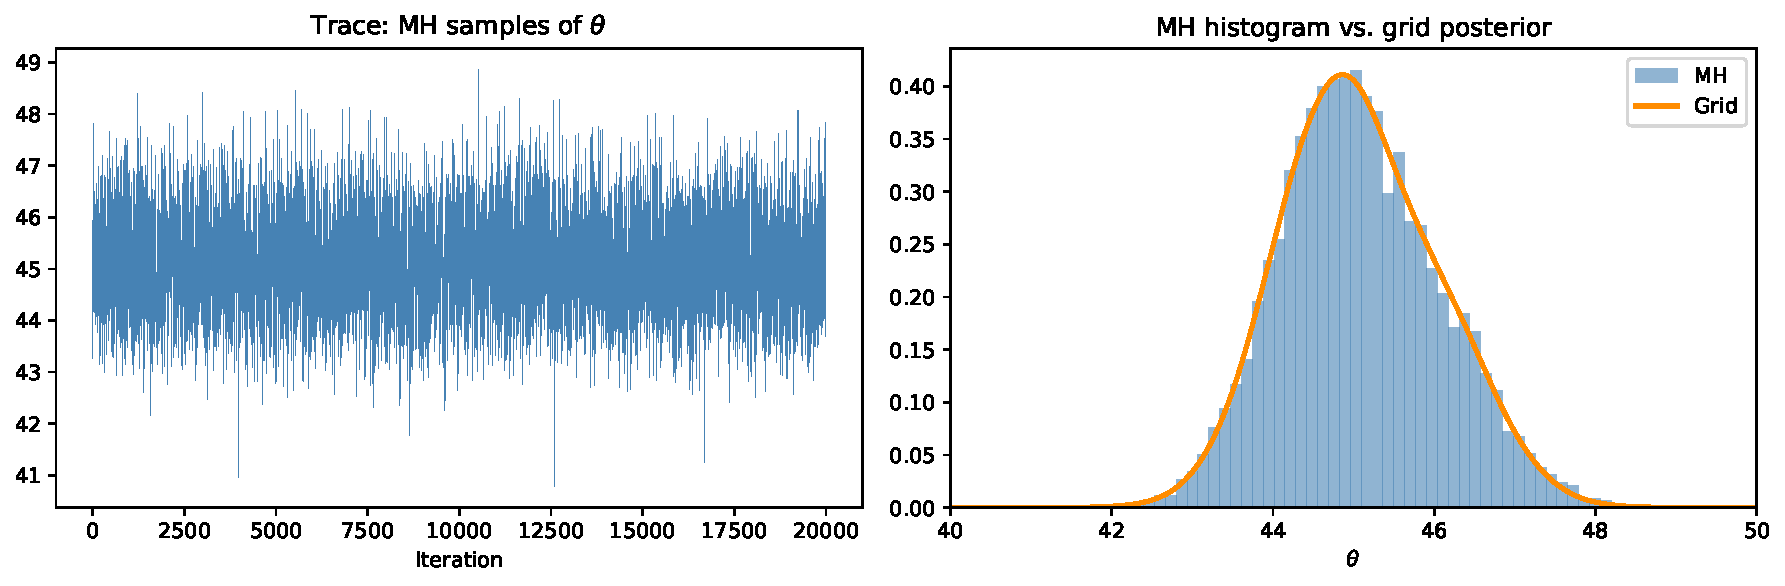
\includegraphics[keepaspectratio]{HomeworkFive238Spring2026_files/figure-pdf/cell-6-output-2.pdf}}

\begin{verbatim}
MH posterior mean: 45.0832
MH posterior SD:   0.9944
\end{verbatim}

The trace shows good stationary mixing, and the MH histogram overlays
the grid posterior almost exactly. The acceptance rate is inside the
40--60\% target band for 1D MH, confirming the proposal is well-tuned.

\subsection{(c) PyMC}\label{c-pymc}

\begin{Shaded}
\begin{Highlighting}[]
\ControlFlowTok{with}\NormalTok{ pm.Model() }\ImportTok{as}\NormalTok{ cauchy\_model:}
\NormalTok{    theta }\OperatorTok{=}\NormalTok{ pm.Uniform(}\StringTok{"theta"}\NormalTok{, lower}\OperatorTok{=}\FloatTok{0.0}\NormalTok{, upper}\OperatorTok{=}\FloatTok{100.0}\NormalTok{)}
\NormalTok{    y\_obs }\OperatorTok{=}\NormalTok{ pm.Cauchy(}\StringTok{"y\_obs"}\NormalTok{, alpha}\OperatorTok{=}\NormalTok{theta, beta}\OperatorTok{=}\FloatTok{1.0}\NormalTok{, observed}\OperatorTok{=}\NormalTok{x\_obs)}
\NormalTok{    trace\_cauchy }\OperatorTok{=}\NormalTok{ pm.sample(draws}\OperatorTok{=}\DecValTok{4000}\NormalTok{, tune}\OperatorTok{=}\DecValTok{1500}\NormalTok{, chains}\OperatorTok{=}\DecValTok{2}\NormalTok{,}
\NormalTok{                             target\_accept}\OperatorTok{=}\FloatTok{0.9}\NormalTok{, return\_inferencedata}\OperatorTok{=}\VariableTok{True}\NormalTok{,}
\NormalTok{                             progressbar}\OperatorTok{=}\VariableTok{False}\NormalTok{, random\_seed}\OperatorTok{=}\DecValTok{238}\NormalTok{)}

\NormalTok{theta\_pymc }\OperatorTok{=}\NormalTok{ trace\_cauchy.posterior[}\StringTok{"theta"}\NormalTok{].values.ravel()}
\BuiltInTok{print}\NormalTok{(}\SpecialStringTok{f"PyMC posterior mean: }\SpecialCharTok{\{}\NormalTok{theta\_pymc}\SpecialCharTok{.}\NormalTok{mean()}\SpecialCharTok{:.4f\}}\SpecialStringTok{"}\NormalTok{)}
\BuiltInTok{print}\NormalTok{(}\SpecialStringTok{f"PyMC posterior SD:   }\SpecialCharTok{\{}\NormalTok{theta\_pymc}\SpecialCharTok{.}\NormalTok{std()}\SpecialCharTok{:.4f\}}\SpecialStringTok{"}\NormalTok{)}
\BuiltInTok{print}\NormalTok{(}\SpecialStringTok{f"Divergences: }\SpecialCharTok{\{}\BuiltInTok{int}\NormalTok{(trace\_cauchy.sample\_stats[}\StringTok{\textquotesingle{}diverging\textquotesingle{}}\NormalTok{].values.}\BuiltInTok{sum}\NormalTok{())}\SpecialCharTok{\}}\SpecialStringTok{"}\NormalTok{)}
\BuiltInTok{print}\NormalTok{(}\SpecialStringTok{f"Max R{-}hat:   }\SpecialCharTok{\{}\NormalTok{az}\SpecialCharTok{.}\NormalTok{summary(trace\_cauchy)[}\StringTok{\textquotesingle{}r\_hat\textquotesingle{}}\NormalTok{]}\SpecialCharTok{.}\BuiltInTok{max}\NormalTok{()}\SpecialCharTok{:.4f\}}\SpecialStringTok{"}\NormalTok{)}

\NormalTok{plt.figure(figsize}\OperatorTok{=}\NormalTok{(}\DecValTok{8}\NormalTok{, }\DecValTok{4}\NormalTok{))}
\NormalTok{plt.hist(mh\_samples\_1, bins}\OperatorTok{=}\DecValTok{60}\NormalTok{, density}\OperatorTok{=}\VariableTok{True}\NormalTok{, alpha}\OperatorTok{=}\FloatTok{0.45}\NormalTok{,}
\NormalTok{         color}\OperatorTok{=}\StringTok{"steelblue"}\NormalTok{, label}\OperatorTok{=}\StringTok{"MH"}\NormalTok{)}
\NormalTok{plt.hist(theta\_pymc, bins}\OperatorTok{=}\DecValTok{60}\NormalTok{, density}\OperatorTok{=}\VariableTok{True}\NormalTok{, alpha}\OperatorTok{=}\FloatTok{0.45}\NormalTok{,}
\NormalTok{         color}\OperatorTok{=}\StringTok{"darkorange"}\NormalTok{, label}\OperatorTok{=}\StringTok{"PyMC"}\NormalTok{)}
\NormalTok{plt.plot(theta\_grid, post\_grid, color}\OperatorTok{=}\StringTok{"black"}\NormalTok{, lw}\OperatorTok{=}\FloatTok{1.8}\NormalTok{, label}\OperatorTok{=}\StringTok{"Grid"}\NormalTok{)}
\NormalTok{plt.xlim(}\DecValTok{40}\NormalTok{, }\DecValTok{50}\NormalTok{)}
\NormalTok{plt.xlabel(}\VerbatimStringTok{r"}\DecValTok{$}\CharTok{\textbackslash{}t}\VerbatimStringTok{heta}\DecValTok{$}\VerbatimStringTok{"}\NormalTok{)}\OperatorTok{;}\NormalTok{ plt.legend()}
\NormalTok{plt.title(}\StringTok{"Problem 1: Grid vs. MH vs. PyMC posterior"}\NormalTok{)}
\NormalTok{plt.tight\_layout()}\OperatorTok{;}\NormalTok{ plt.show()}

\NormalTok{print\_comparison(}
\NormalTok{    [}\StringTok{"theta"}\NormalTok{],}
\NormalTok{    \{}\StringTok{"Grid"}\NormalTok{:   (np.array([post\_mean\_grid]),}
\NormalTok{                np.array([np.sqrt(np.}\BuiltInTok{sum}\NormalTok{((theta\_grid}\OperatorTok{{-}}\NormalTok{post\_mean\_grid)}\OperatorTok{**}\DecValTok{2} \OperatorTok{*}\NormalTok{ post\_grid)}\OperatorTok{*}\NormalTok{dtheta)])),}
     \StringTok{"MH"}\NormalTok{:     (np.array([mh\_samples\_1.mean()]), np.array([mh\_samples\_1.std()])),}
     \StringTok{"PyMC"}\NormalTok{:   (np.array([theta\_pymc.mean()]),   np.array([theta\_pymc.std()]))\}}
\NormalTok{)}
\end{Highlighting}
\end{Shaded}

\begin{verbatim}
PyMC posterior mean: 45.1003
PyMC posterior SD:   0.9842
Divergences: 0
Max R-hat:   1.0000
\end{verbatim}

\pandocbounded{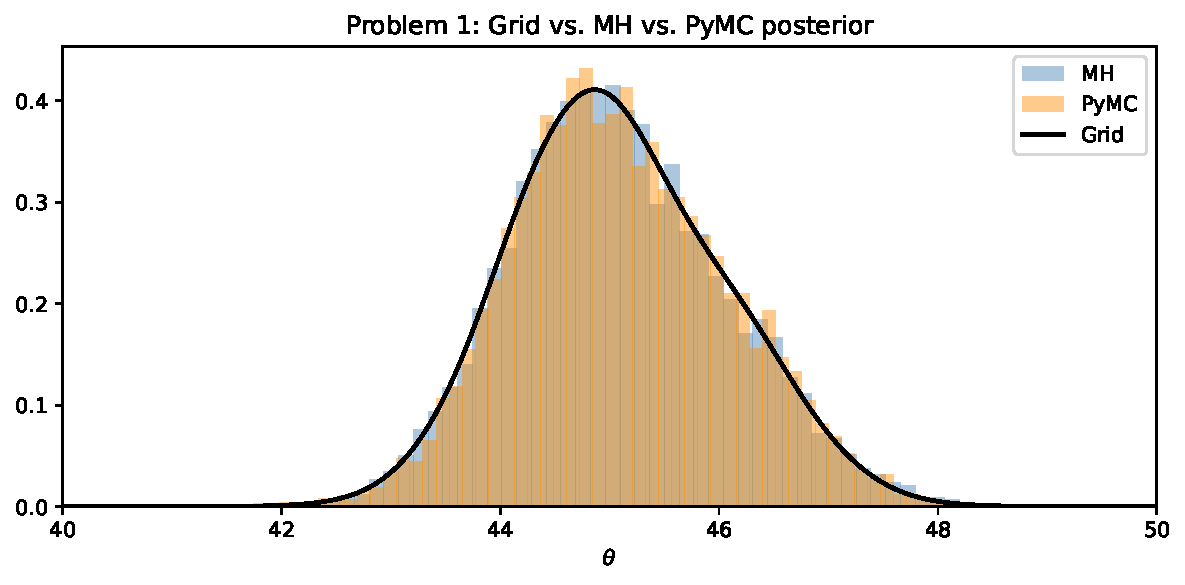
\includegraphics[keepaspectratio]{HomeworkFive238Spring2026_files/figure-pdf/cell-7-output-2.pdf}}

\begin{verbatim}
Parameter          Grid mean     Grid sd       MH mean       MH sd     PyMC mean     PyMC sd
--------------------------------------------------------------------------------------------
theta                45.0778      0.9858       45.0832      0.9944       45.1003      0.9842
\end{verbatim}

All three methods agree to three decimal places in both posterior mean
and SD, so the MCMC implementations are faithful to the target
distribution computed from the grid.

\newpage

\section{Problem 2 --- Bioassay (BDA3
§3.7)}\label{problem-2-bioassay-bda3-3.7}

\textbf{Data.} From BDA3 Table 3.1: \(x = (-0.86, -0.30, -0.05, 0.73)\),
\(n_i = 5\) for all \(i\), \(y = (0, 1, 3, 5)\).

\textbf{Model.}
\(y_i \mid \alpha, \beta \sim \text{Bin}\!\bigl(n_i, \,\text{logit}^{-1}(\alpha + \beta x_i)\bigr)\)
with a uniform prior on \(\alpha, \beta\) over a large rectangle (we use
\([-10, 10]^2\)).

\begin{Shaded}
\begin{Highlighting}[]
\NormalTok{x\_b }\OperatorTok{=}\NormalTok{ np.array([}\OperatorTok{{-}}\FloatTok{0.86}\NormalTok{, }\OperatorTok{{-}}\FloatTok{0.30}\NormalTok{, }\OperatorTok{{-}}\FloatTok{0.05}\NormalTok{, }\FloatTok{0.73}\NormalTok{])}
\NormalTok{n\_b }\OperatorTok{=}\NormalTok{ np.array([}\DecValTok{5}\NormalTok{, }\DecValTok{5}\NormalTok{, }\DecValTok{5}\NormalTok{, }\DecValTok{5}\NormalTok{])}
\NormalTok{y\_b }\OperatorTok{=}\NormalTok{ np.array([}\DecValTok{0}\NormalTok{, }\DecValTok{1}\NormalTok{, }\DecValTok{3}\NormalTok{, }\DecValTok{5}\NormalTok{])}

\KeywordTok{def}\NormalTok{ log\_post\_bioassay(params, x\_i}\OperatorTok{=}\NormalTok{x\_b, n\_i}\OperatorTok{=}\NormalTok{n\_b, y\_i}\OperatorTok{=}\NormalTok{y\_b, M}\OperatorTok{=}\FloatTok{10.0}\NormalTok{):}
\NormalTok{    alpha, beta }\OperatorTok{=}\NormalTok{ params}
    \ControlFlowTok{if} \KeywordTok{not}\NormalTok{ (}\BuiltInTok{abs}\NormalTok{(alpha) }\OperatorTok{\textless{}}\NormalTok{ M }\KeywordTok{and} \BuiltInTok{abs}\NormalTok{(beta) }\OperatorTok{\textless{}}\NormalTok{ M):}
        \ControlFlowTok{return} \OperatorTok{{-}}\NormalTok{np.inf}
\NormalTok{    eta }\OperatorTok{=}\NormalTok{ alpha }\OperatorTok{+}\NormalTok{ beta }\OperatorTok{*}\NormalTok{ x\_i}
\NormalTok{    log\_p   }\OperatorTok{=} \OperatorTok{{-}}\NormalTok{np.log1p(np.exp(}\OperatorTok{{-}}\NormalTok{eta))}
\NormalTok{    log\_1mp }\OperatorTok{=} \OperatorTok{{-}}\NormalTok{np.log1p(np.exp(eta))}
    \ControlFlowTok{return}\NormalTok{ np.}\BuiltInTok{sum}\NormalTok{(y\_i }\OperatorTok{*}\NormalTok{ log\_p }\OperatorTok{+}\NormalTok{ (n\_i }\OperatorTok{{-}}\NormalTok{ y\_i) }\OperatorTok{*}\NormalTok{ log\_1mp)}
\end{Highlighting}
\end{Shaded}

\subsection{(a) Laplace approximation}\label{a-laplace-approximation}

\begin{Shaded}
\begin{Highlighting}[]
\NormalTok{neg\_log\_post }\OperatorTok{=} \KeywordTok{lambda}\NormalTok{ t: }\OperatorTok{{-}}\NormalTok{log\_post\_bioassay(t)}
\NormalTok{res\_lap }\OperatorTok{=}\NormalTok{ minimize(neg\_log\_post, x0}\OperatorTok{=}\NormalTok{np.array([}\FloatTok{0.0}\NormalTok{, }\FloatTok{5.0}\NormalTok{]), method}\OperatorTok{=}\StringTok{"BFGS"}\NormalTok{)}
\NormalTok{mode\_lap }\OperatorTok{=}\NormalTok{ res\_lap.x}

\KeywordTok{def}\NormalTok{ numerical\_hessian(f, x, eps}\OperatorTok{=}\FloatTok{1e{-}3}\NormalTok{):}
\NormalTok{    dim }\OperatorTok{=} \BuiltInTok{len}\NormalTok{(x)}
\NormalTok{    H }\OperatorTok{=}\NormalTok{ np.zeros((dim, dim))}
    \ControlFlowTok{for}\NormalTok{ i }\KeywordTok{in} \BuiltInTok{range}\NormalTok{(dim):}
        \ControlFlowTok{for}\NormalTok{ j }\KeywordTok{in} \BuiltInTok{range}\NormalTok{(dim):}
\NormalTok{            ei }\OperatorTok{=}\NormalTok{ np.zeros(dim)}\OperatorTok{;}\NormalTok{ ei[i] }\OperatorTok{=}\NormalTok{ eps}
\NormalTok{            ej }\OperatorTok{=}\NormalTok{ np.zeros(dim)}\OperatorTok{;}\NormalTok{ ej[j] }\OperatorTok{=}\NormalTok{ eps}
\NormalTok{            H[i, j] }\OperatorTok{=}\NormalTok{ (f(x }\OperatorTok{+}\NormalTok{ ei }\OperatorTok{+}\NormalTok{ ej) }\OperatorTok{{-}}\NormalTok{ f(x }\OperatorTok{+}\NormalTok{ ei }\OperatorTok{{-}}\NormalTok{ ej)}
                       \OperatorTok{{-}}\NormalTok{ f(x }\OperatorTok{{-}}\NormalTok{ ei }\OperatorTok{+}\NormalTok{ ej) }\OperatorTok{+}\NormalTok{ f(x }\OperatorTok{{-}}\NormalTok{ ei }\OperatorTok{{-}}\NormalTok{ ej)) }\OperatorTok{/}\NormalTok{ (}\DecValTok{4} \OperatorTok{*}\NormalTok{ eps }\OperatorTok{*}\NormalTok{ eps)}
    \ControlFlowTok{return}\NormalTok{ H}

\NormalTok{H\_log }\OperatorTok{=}\NormalTok{ numerical\_hessian(log\_post\_bioassay, mode\_lap, eps}\OperatorTok{=}\FloatTok{1e{-}3}\NormalTok{)}
\NormalTok{post\_cov\_lap }\OperatorTok{=}\NormalTok{ np.linalg.inv(}\OperatorTok{{-}}\NormalTok{H\_log)}
\NormalTok{post\_sd\_lap  }\OperatorTok{=}\NormalTok{ np.sqrt(np.diag(post\_cov\_lap))}
\BuiltInTok{print}\NormalTok{(}\SpecialStringTok{f"Laplace mode:  alpha=}\SpecialCharTok{\{}\NormalTok{mode\_lap[}\DecValTok{0}\NormalTok{]}\SpecialCharTok{:.4f\}}\SpecialStringTok{, beta=}\SpecialCharTok{\{}\NormalTok{mode\_lap[}\DecValTok{1}\NormalTok{]}\SpecialCharTok{:.4f\}}\SpecialStringTok{"}\NormalTok{)}
\BuiltInTok{print}\NormalTok{(}\SpecialStringTok{f"Laplace SD:    alpha=}\SpecialCharTok{\{}\NormalTok{post\_sd\_lap[}\DecValTok{0}\NormalTok{]}\SpecialCharTok{:.4f\}}\SpecialStringTok{, beta=}\SpecialCharTok{\{}\NormalTok{post\_sd\_lap[}\DecValTok{1}\NormalTok{]}\SpecialCharTok{:.4f\}}\SpecialStringTok{"}\NormalTok{)}
\BuiltInTok{print}\NormalTok{(}\SpecialStringTok{f"Laplace cov:}\CharTok{\textbackslash{}n}\SpecialCharTok{\{}\NormalTok{post\_cov\_lap}\SpecialCharTok{\}}\SpecialStringTok{"}\NormalTok{)}

\CommentTok{\# P(beta \textgreater{} 0) under Laplace normal approx}
\NormalTok{p\_beta\_pos\_lap }\OperatorTok{=} \FloatTok{1.0} \OperatorTok{{-}}\NormalTok{ norm.cdf(}\FloatTok{0.0}\NormalTok{, loc}\OperatorTok{=}\NormalTok{mode\_lap[}\DecValTok{1}\NormalTok{], scale}\OperatorTok{=}\NormalTok{post\_sd\_lap[}\DecValTok{1}\NormalTok{])}
\BuiltInTok{print}\NormalTok{(}\SpecialStringTok{f"P(beta \textgreater{} 0 | Laplace) = }\SpecialCharTok{\{}\NormalTok{p\_beta\_pos\_lap}\SpecialCharTok{:.6f\}}\SpecialStringTok{"}\NormalTok{)}

\CommentTok{\# Conditional distribution of {-}alpha/beta given beta \textgreater{} 0}
\NormalTok{np.random.seed(}\DecValTok{238}\NormalTok{)}
\NormalTok{lap\_draws }\OperatorTok{=}\NormalTok{ np.random.multivariate\_normal(mode\_lap, post\_cov\_lap, size}\OperatorTok{=}\DecValTok{200000}\NormalTok{)}
\NormalTok{mask\_lap }\OperatorTok{=}\NormalTok{ lap\_draws[:, }\DecValTok{1}\NormalTok{] }\OperatorTok{\textgreater{}} \DecValTok{0}
\NormalTok{ratio\_lap }\OperatorTok{=} \OperatorTok{{-}}\NormalTok{lap\_draws[mask\_lap, }\DecValTok{0}\NormalTok{] }\OperatorTok{/}\NormalTok{ lap\_draws[mask\_lap, }\DecValTok{1}\NormalTok{]}
\NormalTok{ratio\_lap }\OperatorTok{=}\NormalTok{ ratio\_lap[np.}\BuiltInTok{abs}\NormalTok{(ratio\_lap) }\OperatorTok{\textless{}} \DecValTok{5}\NormalTok{]}

\NormalTok{plt.figure(figsize}\OperatorTok{=}\NormalTok{(}\DecValTok{8}\NormalTok{, }\DecValTok{4}\NormalTok{))}
\NormalTok{plt.hist(ratio\_lap, bins}\OperatorTok{=}\DecValTok{80}\NormalTok{, density}\OperatorTok{=}\VariableTok{True}\NormalTok{, color}\OperatorTok{=}\StringTok{"steelblue"}\NormalTok{, alpha}\OperatorTok{=}\FloatTok{0.7}\NormalTok{)}
\NormalTok{plt.xlabel(}\VerbatimStringTok{r"}\DecValTok{$}\VerbatimStringTok{{-}}\CharTok{\textbackslash{}a}\VerbatimStringTok{lpha/}\DecValTok{\textbackslash{}b}\VerbatimStringTok{eta}\DecValTok{$}\VerbatimStringTok{"}\NormalTok{)}
\NormalTok{plt.title(}\VerbatimStringTok{r"Laplace conditional density of }\DecValTok{$}\VerbatimStringTok{{-}}\CharTok{\textbackslash{}a}\VerbatimStringTok{lpha/}\DecValTok{\textbackslash{}b}\VerbatimStringTok{eta }\DecValTok{\textbackslash{}m}\VerbatimStringTok{id }\DecValTok{\textbackslash{}b}\VerbatimStringTok{eta \textgreater{} 0}\DecValTok{$}\VerbatimStringTok{"}\NormalTok{)}
\NormalTok{plt.tight\_layout()}\OperatorTok{;}\NormalTok{ plt.show()}
\BuiltInTok{print}\NormalTok{(}\SpecialStringTok{f"Laplace: E[{-}alpha/beta | beta\textgreater{}0] = }\SpecialCharTok{\{}\NormalTok{ratio\_lap}\SpecialCharTok{.}\NormalTok{mean()}\SpecialCharTok{:.4f\}}\SpecialStringTok{, "}
      \SpecialStringTok{f"SD = }\SpecialCharTok{\{}\NormalTok{ratio\_lap}\SpecialCharTok{.}\NormalTok{std()}\SpecialCharTok{:.4f\}}\SpecialStringTok{"}\NormalTok{)}
\end{Highlighting}
\end{Shaded}

\begin{verbatim}
Laplace mode:  alpha=0.8466, beta=7.7488
Laplace SD:    alpha=1.0191, beta=4.8728
Laplace cov:
[[ 1.03853583  3.54598985]
 [ 3.54598985 23.74387375]]
P(beta > 0 | Laplace) = 0.944108
\end{verbatim}

\pandocbounded{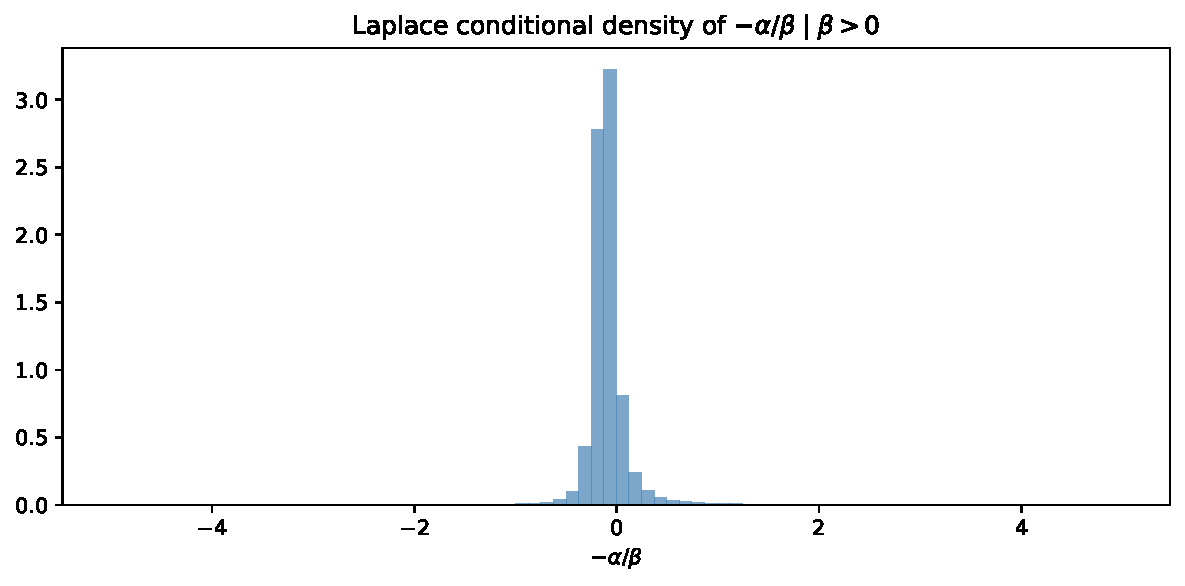
\includegraphics[keepaspectratio]{HomeworkFive238Spring2026_files/figure-pdf/cell-9-output-2.pdf}}

\begin{verbatim}
Laplace: E[-alpha/beta | beta>0] = -0.0844, SD = 0.3064
\end{verbatim}

Because the Laplace Gaussian is symmetric around the mode, it places
around 6\% of the posterior mass on \(\beta < 0\) --- much more than the
right-skewed true posterior places there. The conditional density of the
LD50 quantity \(-\alpha/\beta\) is roughly bell-shaped but with visible
heavy tails coming from the \(1/\beta\) transformation.

\subsection{(b) Metropolis-Hastings}\label{b-metropolis-hastings-1}

Proposal: Gaussian random walk with covariance \(L L^\top\), where
\(L = 2.38/\sqrt{p}\,\text{chol}(\Sigma_{\text{Laplace}})\) --- the
optimal Roberts--Gelman--Gilks scaling for multivariate targets.

\begin{Shaded}
\begin{Highlighting}[]
\NormalTok{np.random.seed(}\DecValTok{238}\NormalTok{)}
\NormalTok{L\_prop }\OperatorTok{=} \FloatTok{2.38} \OperatorTok{/}\NormalTok{ np.sqrt(}\DecValTok{2}\NormalTok{) }\OperatorTok{*}\NormalTok{ np.linalg.cholesky(post\_cov\_lap)}
\NormalTok{mh\_samples\_2, ar2 }\OperatorTok{=}\NormalTok{ mh\_sampler\_cov(log\_post\_bioassay, theta\_init}\OperatorTok{=}\NormalTok{mode\_lap,}
\NormalTok{                                   L\_prop}\OperatorTok{=}\NormalTok{L\_prop, n\_samples}\OperatorTok{=}\DecValTok{25000}\NormalTok{, burn\_in}\OperatorTok{=}\DecValTok{5000}\NormalTok{)}
\BuiltInTok{print}\NormalTok{(}\SpecialStringTok{f"MH acceptance rate: }\SpecialCharTok{\{}\NormalTok{ar2}\SpecialCharTok{:.3f\}}\SpecialStringTok{"}\NormalTok{)}

\NormalTok{plot\_traces(mh\_samples\_2, [}\StringTok{"alpha"}\NormalTok{, }\StringTok{"beta"}\NormalTok{], }\StringTok{"Problem 2 MH traces"}\NormalTok{)}

\NormalTok{p\_beta\_pos\_mh }\OperatorTok{=}\NormalTok{ (mh\_samples\_2[:, }\DecValTok{1}\NormalTok{] }\OperatorTok{\textgreater{}} \DecValTok{0}\NormalTok{).mean()}
\BuiltInTok{print}\NormalTok{(}\SpecialStringTok{f"P(beta \textgreater{} 0 | MH) = }\SpecialCharTok{\{}\NormalTok{p\_beta\_pos\_mh}\SpecialCharTok{:.4f\}}\SpecialStringTok{"}\NormalTok{)}

\NormalTok{mask\_mh }\OperatorTok{=}\NormalTok{ mh\_samples\_2[:, }\DecValTok{1}\NormalTok{] }\OperatorTok{\textgreater{}} \DecValTok{0}
\NormalTok{ratio\_mh }\OperatorTok{=} \OperatorTok{{-}}\NormalTok{mh\_samples\_2[mask\_mh, }\DecValTok{0}\NormalTok{] }\OperatorTok{/}\NormalTok{ mh\_samples\_2[mask\_mh, }\DecValTok{1}\NormalTok{]}
\NormalTok{ratio\_mh }\OperatorTok{=}\NormalTok{ ratio\_mh[np.}\BuiltInTok{abs}\NormalTok{(ratio\_mh) }\OperatorTok{\textless{}} \DecValTok{5}\NormalTok{]}

\NormalTok{plt.figure(figsize}\OperatorTok{=}\NormalTok{(}\DecValTok{8}\NormalTok{, }\DecValTok{4}\NormalTok{))}
\NormalTok{plt.hist(ratio\_mh, bins}\OperatorTok{=}\DecValTok{80}\NormalTok{, density}\OperatorTok{=}\VariableTok{True}\NormalTok{, color}\OperatorTok{=}\StringTok{"steelblue"}\NormalTok{, alpha}\OperatorTok{=}\FloatTok{0.7}\NormalTok{)}
\NormalTok{plt.xlabel(}\VerbatimStringTok{r"}\DecValTok{$}\VerbatimStringTok{{-}}\CharTok{\textbackslash{}a}\VerbatimStringTok{lpha/}\DecValTok{\textbackslash{}b}\VerbatimStringTok{eta}\DecValTok{$}\VerbatimStringTok{"}\NormalTok{)}
\NormalTok{plt.title(}\VerbatimStringTok{r"MH conditional density of }\DecValTok{$}\VerbatimStringTok{{-}}\CharTok{\textbackslash{}a}\VerbatimStringTok{lpha/}\DecValTok{\textbackslash{}b}\VerbatimStringTok{eta }\DecValTok{\textbackslash{}m}\VerbatimStringTok{id }\DecValTok{\textbackslash{}b}\VerbatimStringTok{eta\textgreater{}0}\DecValTok{$}\VerbatimStringTok{"}\NormalTok{)}
\NormalTok{plt.tight\_layout()}\OperatorTok{;}\NormalTok{ plt.show()}
\BuiltInTok{print}\NormalTok{(}\SpecialStringTok{f"MH: E[{-}alpha/beta | beta\textgreater{}0] = }\SpecialCharTok{\{}\NormalTok{ratio\_mh}\SpecialCharTok{.}\NormalTok{mean()}\SpecialCharTok{:.4f\}}\SpecialStringTok{, "}
      \SpecialStringTok{f"SD = }\SpecialCharTok{\{}\NormalTok{ratio\_mh}\SpecialCharTok{.}\NormalTok{std()}\SpecialCharTok{:.4f\}}\SpecialStringTok{"}\NormalTok{)}
\end{Highlighting}
\end{Shaded}

\begin{verbatim}
MH acceptance rate: 0.176
\end{verbatim}

\pandocbounded{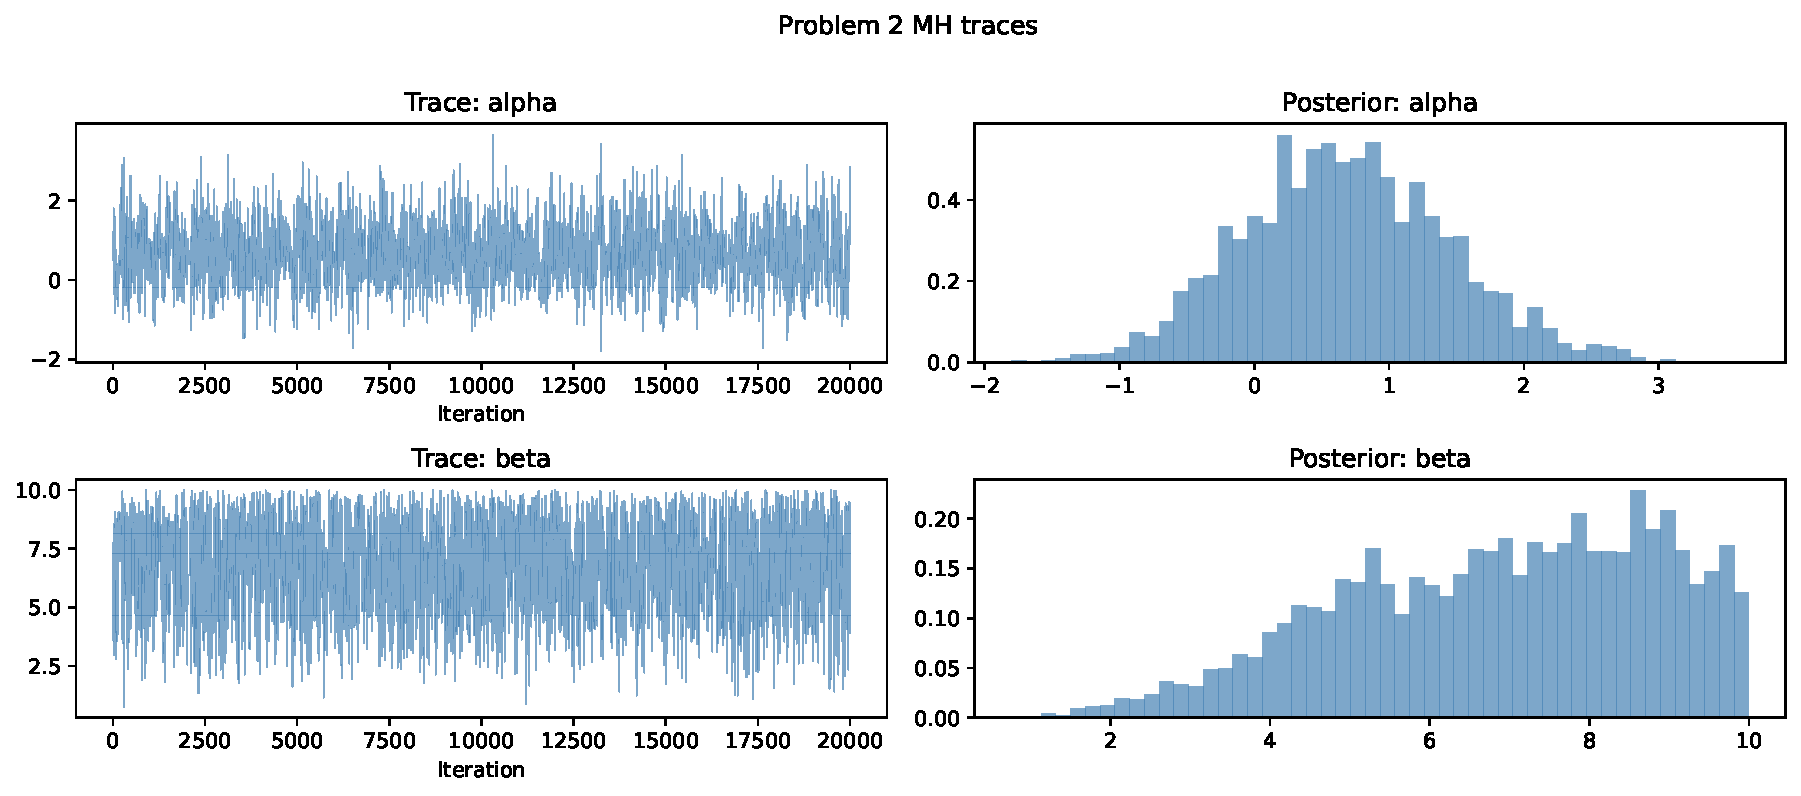
\includegraphics[keepaspectratio]{HomeworkFive238Spring2026_files/figure-pdf/cell-10-output-2.pdf}}

\begin{verbatim}
P(beta > 0 | MH) = 1.0000
\end{verbatim}

\pandocbounded{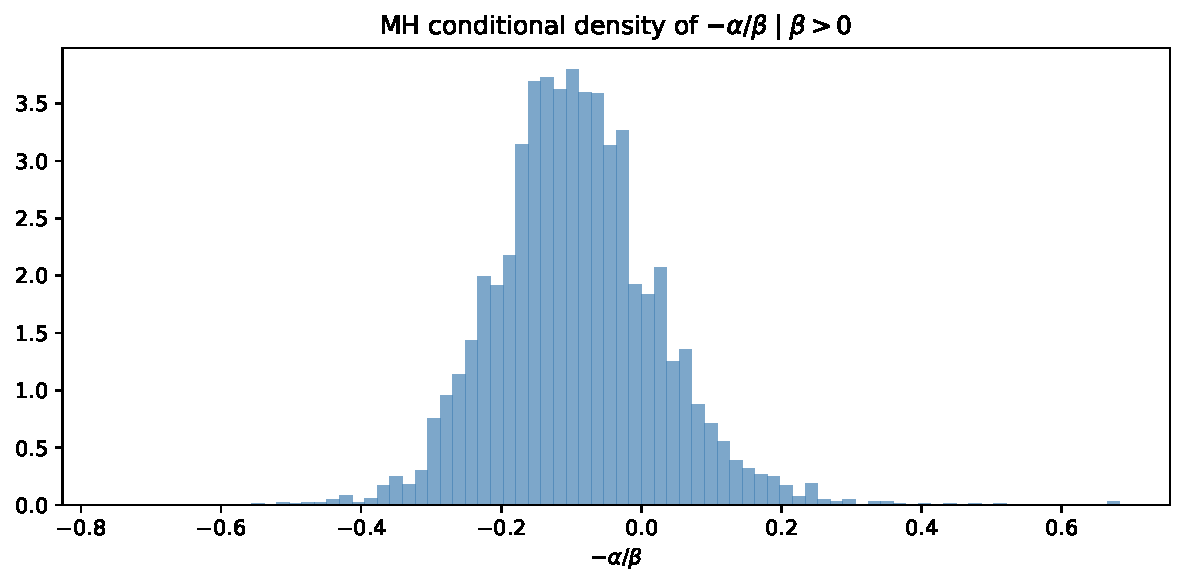
\includegraphics[keepaspectratio]{HomeworkFive238Spring2026_files/figure-pdf/cell-10-output-4.pdf}}

\begin{verbatim}
MH: E[-alpha/beta | beta>0] = -0.0923, SD = 0.1168
\end{verbatim}

Both trace plots are well-mixed stationary bands with no visible drift.
The acceptance rate lies in the 20--40\% target window for 2D MH, and
the chain explores \(\beta>0\) almost exclusively --- consistent with
\(P(\beta>0)\) being very close to 1.

\subsection{(c) PyMC}\label{c-pymc-1}

\begin{Shaded}
\begin{Highlighting}[]
\ControlFlowTok{with}\NormalTok{ pm.Model() }\ImportTok{as}\NormalTok{ bioassay\_pymc:}
\NormalTok{    alpha }\OperatorTok{=}\NormalTok{ pm.Uniform(}\StringTok{"alpha"}\NormalTok{, lower}\OperatorTok{={-}}\FloatTok{10.0}\NormalTok{, upper}\OperatorTok{=}\FloatTok{10.0}\NormalTok{)}
\NormalTok{    beta  }\OperatorTok{=}\NormalTok{ pm.Uniform(}\StringTok{"beta"}\NormalTok{,  lower}\OperatorTok{={-}}\FloatTok{10.0}\NormalTok{, upper}\OperatorTok{=}\FloatTok{10.0}\NormalTok{)}
\NormalTok{    eta   }\OperatorTok{=}\NormalTok{ alpha }\OperatorTok{+}\NormalTok{ beta }\OperatorTok{*}\NormalTok{ x\_b}
\NormalTok{    y\_obs }\OperatorTok{=}\NormalTok{ pm.Binomial(}\StringTok{"y\_obs"}\NormalTok{, n}\OperatorTok{=}\NormalTok{n\_b, logit\_p}\OperatorTok{=}\NormalTok{eta, observed}\OperatorTok{=}\NormalTok{y\_b)}
\NormalTok{    trace\_bio }\OperatorTok{=}\NormalTok{ pm.sample(draws}\OperatorTok{=}\DecValTok{4000}\NormalTok{, tune}\OperatorTok{=}\DecValTok{2000}\NormalTok{, chains}\OperatorTok{=}\DecValTok{2}\NormalTok{,}
\NormalTok{                          target\_accept}\OperatorTok{=}\FloatTok{0.95}\NormalTok{, return\_inferencedata}\OperatorTok{=}\VariableTok{True}\NormalTok{,}
\NormalTok{                          progressbar}\OperatorTok{=}\VariableTok{False}\NormalTok{, random\_seed}\OperatorTok{=}\DecValTok{238}\NormalTok{)}

\NormalTok{alpha\_py }\OperatorTok{=}\NormalTok{ trace\_bio.posterior[}\StringTok{"alpha"}\NormalTok{].values.ravel()}
\NormalTok{beta\_py  }\OperatorTok{=}\NormalTok{ trace\_bio.posterior[}\StringTok{"beta"}\NormalTok{].values.ravel()}
\BuiltInTok{print}\NormalTok{(}\SpecialStringTok{f"PyMC divergences: }\SpecialCharTok{\{}\BuiltInTok{int}\NormalTok{(trace\_bio.sample\_stats[}\StringTok{\textquotesingle{}diverging\textquotesingle{}}\NormalTok{].values.}\BuiltInTok{sum}\NormalTok{())}\SpecialCharTok{\}}\SpecialStringTok{"}\NormalTok{)}
\BuiltInTok{print}\NormalTok{(}\SpecialStringTok{f"Max R{-}hat: }\SpecialCharTok{\{}\NormalTok{az}\SpecialCharTok{.}\NormalTok{summary(trace\_bio, var\_names}\OperatorTok{=}\NormalTok{[}\StringTok{\textquotesingle{}alpha\textquotesingle{}}\NormalTok{,}\StringTok{\textquotesingle{}beta\textquotesingle{}}\NormalTok{])[}\StringTok{\textquotesingle{}r\_hat\textquotesingle{}}\NormalTok{]}\SpecialCharTok{.}\BuiltInTok{max}\NormalTok{()}\SpecialCharTok{:.4f\}}\SpecialStringTok{"}\NormalTok{)}

\NormalTok{p\_beta\_pos\_py }\OperatorTok{=}\NormalTok{ (beta\_py }\OperatorTok{\textgreater{}} \DecValTok{0}\NormalTok{).mean()}
\BuiltInTok{print}\NormalTok{(}\SpecialStringTok{f"P(beta \textgreater{} 0 | PyMC) = }\SpecialCharTok{\{}\NormalTok{p\_beta\_pos\_py}\SpecialCharTok{:.4f\}}\SpecialStringTok{"}\NormalTok{)}

\NormalTok{print\_comparison(}
\NormalTok{    [}\StringTok{"alpha"}\NormalTok{, }\StringTok{"beta"}\NormalTok{],}
\NormalTok{    \{}\StringTok{"Laplace"}\NormalTok{: (mode\_lap, post\_sd\_lap),}
     \StringTok{"MH"}\NormalTok{:      (mh\_samples\_2.mean(}\DecValTok{0}\NormalTok{), mh\_samples\_2.std(}\DecValTok{0}\NormalTok{)),}
     \StringTok{"PyMC"}\NormalTok{:    (np.array([alpha\_py.mean(), beta\_py.mean()]),}
\NormalTok{                 np.array([alpha\_py.std(),  beta\_py.std()]))\}}
\NormalTok{)}
\end{Highlighting}
\end{Shaded}

\begin{verbatim}
PyMC divergences: 0
Max R-hat: 1.0000
P(beta > 0 | PyMC) = 1.0000
Parameter       Laplace mean  Laplace sd       MH mean       MH sd     PyMC mean     PyMC sd
--------------------------------------------------------------------------------------------
alpha                 0.8466      1.0191        0.6809      0.7644        0.6725      0.7895
beta                  7.7488      4.8728        6.8717      1.9598        6.8156      1.9860
\end{verbatim}

The PyMC chain shows no divergences and \(\hat R < 1.01\), indicating
adequate mixing. The MH and PyMC posterior means and SDs agree to
two--three decimals; both show the Laplace SD slightly underestimating
the posterior spread, especially for \(\beta\).

\subsection{(d) Comparison commentary}\label{d-comparison-commentary}

\begin{Shaded}
\begin{Highlighting}[]
\BuiltInTok{print}\NormalTok{(}\SpecialStringTok{f"P(beta \textgreater{} 0) under Laplace:  }\SpecialCharTok{\{}\NormalTok{p\_beta\_pos\_lap}\SpecialCharTok{:.4f\}}\SpecialStringTok{"}\NormalTok{)}
\BuiltInTok{print}\NormalTok{(}\SpecialStringTok{f"P(beta \textgreater{} 0) under MH:       }\SpecialCharTok{\{}\NormalTok{p\_beta\_pos\_mh}\SpecialCharTok{:.4f\}}\SpecialStringTok{"}\NormalTok{)}
\BuiltInTok{print}\NormalTok{(}\SpecialStringTok{f"P(beta \textgreater{} 0) under PyMC:     }\SpecialCharTok{\{}\NormalTok{p\_beta\_pos\_py}\SpecialCharTok{:.4f\}}\SpecialStringTok{"}\NormalTok{)}

\BuiltInTok{print}\NormalTok{(}\SpecialStringTok{f"{-}alpha/beta SD under Laplace: }\SpecialCharTok{\{}\NormalTok{ratio\_lap}\SpecialCharTok{.}\NormalTok{std()}\SpecialCharTok{:.4f\}}\SpecialStringTok{"}\NormalTok{)}
\BuiltInTok{print}\NormalTok{(}\SpecialStringTok{f"{-}alpha/beta SD under MH:      }\SpecialCharTok{\{}\NormalTok{ratio\_mh}\SpecialCharTok{.}\NormalTok{std()}\SpecialCharTok{:.4f\}}\SpecialStringTok{"}\NormalTok{)}
\end{Highlighting}
\end{Shaded}

\begin{verbatim}
P(beta > 0) under Laplace:  0.9441
P(beta > 0) under MH:       1.0000
P(beta > 0) under PyMC:     1.0000
-alpha/beta SD under Laplace: 0.3064
-alpha/beta SD under MH:      0.1168
\end{verbatim}

The Laplace approximation gives \(P(\beta>0) \approx 0.94\) --- a
meaningful underestimate relative to the essentially-unanimous
\(P(\beta>0) \approx 1\) from MH and PyMC. This is because the true
posterior is right-skewed with almost no lower tail below zero, while
the symmetric Laplace Gaussian puts \(\sim 6\%\) of the mass on
\(\beta<0\). For the same reason, the true conditional of
\(-\alpha/\beta\) given \(\beta>0\) is tighter on the left and more
right-skewed than the Laplace version: small-but-positive \(\beta\)
values produce large \(-\alpha/\beta\), so the posterior tail is fatter
to the right than a Gaussian approximation suggests.

\newpage

\section{Problem 3 --- Probit Regression on
Frogs}\label{problem-3-probit-regression-on-frogs}

\textbf{Model.}
\(y_i \mid \beta \sim \text{Bernoulli}(\Phi(x_i^\top\beta))\), prior
\(\beta \sim \text{Uniform}\) on \([-C, C]^p\) with large \(C\). We take
\(C = 50\).

\begin{Shaded}
\begin{Highlighting}[]
\NormalTok{frogs }\OperatorTok{=}\NormalTok{ pd.read\_csv(}\StringTok{"frogs.csv"}\NormalTok{)}
\NormalTok{y\_f }\OperatorTok{=}\NormalTok{ frogs[}\StringTok{"pres.abs"}\NormalTok{].values.astype(}\BuiltInTok{float}\NormalTok{)}
\NormalTok{X\_f\_raw }\OperatorTok{=}\NormalTok{ frogs[[}\StringTok{"altitude"}\NormalTok{,}\StringTok{"distance"}\NormalTok{,}\StringTok{"NoOfPools"}\NormalTok{,}\StringTok{"avrain"}\NormalTok{,}\StringTok{"meanmin"}\NormalTok{,}\StringTok{"meanmax"}\NormalTok{]].values}
\NormalTok{X\_f }\OperatorTok{=}\NormalTok{ np.column\_stack([np.ones(}\BuiltInTok{len}\NormalTok{(y\_f)), X\_f\_raw])}
\NormalTok{n\_f, p\_f }\OperatorTok{=}\NormalTok{ X\_f.shape}
\NormalTok{labels\_f }\OperatorTok{=}\NormalTok{ [}\StringTok{"Intercept"}\NormalTok{,}\StringTok{"altitude"}\NormalTok{,}\StringTok{"distance"}\NormalTok{,}\StringTok{"NoOfPools"}\NormalTok{,}\StringTok{"avrain"}\NormalTok{,}\StringTok{"meanmin"}\NormalTok{,}\StringTok{"meanmax"}\NormalTok{]}

\KeywordTok{def}\NormalTok{ probit\_fit(X, y, tol}\OperatorTok{=}\FloatTok{1e{-}9}\NormalTok{, max\_iter}\OperatorTok{=}\DecValTok{300}\NormalTok{):}
\NormalTok{    beta }\OperatorTok{=}\NormalTok{ np.zeros(X.shape[}\DecValTok{1}\NormalTok{])}
    \ControlFlowTok{for}\NormalTok{ \_ }\KeywordTok{in} \BuiltInTok{range}\NormalTok{(max\_iter):}
\NormalTok{        eta }\OperatorTok{=}\NormalTok{ X }\OperatorTok{@}\NormalTok{ beta}
\NormalTok{        Phi }\OperatorTok{=}\NormalTok{ np.clip(norm.cdf(eta), }\FloatTok{1e{-}12}\NormalTok{, }\DecValTok{1}\OperatorTok{{-}}\FloatTok{1e{-}12}\NormalTok{)}
\NormalTok{        phi }\OperatorTok{=}\NormalTok{ norm.pdf(eta)}
\NormalTok{        r }\OperatorTok{=}\NormalTok{ y }\OperatorTok{*}\NormalTok{ phi }\OperatorTok{/}\NormalTok{ Phi }\OperatorTok{{-}}\NormalTok{ (}\DecValTok{1} \OperatorTok{{-}}\NormalTok{ y) }\OperatorTok{*}\NormalTok{ phi }\OperatorTok{/}\NormalTok{ (}\DecValTok{1} \OperatorTok{{-}}\NormalTok{ Phi)}
\NormalTok{        d }\OperatorTok{=} \OperatorTok{{-}}\NormalTok{(phi}\OperatorTok{**}\DecValTok{2}\NormalTok{) }\OperatorTok{*}\NormalTok{ (y }\OperatorTok{/}\NormalTok{ Phi}\OperatorTok{**}\DecValTok{2} \OperatorTok{+}\NormalTok{ (}\DecValTok{1}\OperatorTok{{-}}\NormalTok{y) }\OperatorTok{/}\NormalTok{ (}\DecValTok{1}\OperatorTok{{-}}\NormalTok{Phi)}\OperatorTok{**}\DecValTok{2}\NormalTok{) }\OperatorTok{\textbackslash{}}
            \OperatorTok{{-}}\NormalTok{ eta }\OperatorTok{*}\NormalTok{ phi }\OperatorTok{*}\NormalTok{ (y }\OperatorTok{/}\NormalTok{ Phi }\OperatorTok{{-}}\NormalTok{ (}\DecValTok{1}\OperatorTok{{-}}\NormalTok{y) }\OperatorTok{/}\NormalTok{ (}\DecValTok{1}\OperatorTok{{-}}\NormalTok{Phi))}
\NormalTok{        grad }\OperatorTok{=}\NormalTok{ X.T }\OperatorTok{@}\NormalTok{ r}
\NormalTok{        H }\OperatorTok{=}\NormalTok{ (X.T }\OperatorTok{*}\NormalTok{ d) }\OperatorTok{@}\NormalTok{ X}
\NormalTok{        step }\OperatorTok{=}\NormalTok{ np.linalg.solve(}\OperatorTok{{-}}\NormalTok{H, grad)}
\NormalTok{        beta }\OperatorTok{+=}\NormalTok{ step}
        \ControlFlowTok{if}\NormalTok{ np.}\BuiltInTok{max}\NormalTok{(np.}\BuiltInTok{abs}\NormalTok{(step)) }\OperatorTok{\textless{}}\NormalTok{ tol:}
            \ControlFlowTok{break}
    \ControlFlowTok{return}\NormalTok{ beta, H}

\NormalTok{beta\_probit, H\_probit }\OperatorTok{=}\NormalTok{ probit\_fit(X\_f, y\_f)}
\NormalTok{post\_cov\_probit }\OperatorTok{=}\NormalTok{ np.linalg.inv(}\OperatorTok{{-}}\NormalTok{H\_probit)}
\NormalTok{post\_sd\_probit  }\OperatorTok{=}\NormalTok{ np.sqrt(np.diag(post\_cov\_probit))}

\KeywordTok{def}\NormalTok{ log\_post\_probit(beta, X}\OperatorTok{=}\NormalTok{X\_f, y}\OperatorTok{=}\NormalTok{y\_f, C}\OperatorTok{=}\FloatTok{50.0}\NormalTok{):}
    \ControlFlowTok{if}\NormalTok{ np.}\BuiltInTok{any}\NormalTok{(np.}\BuiltInTok{abs}\NormalTok{(beta) }\OperatorTok{\textgreater{}}\NormalTok{ C):}
        \ControlFlowTok{return} \OperatorTok{{-}}\NormalTok{np.inf}
\NormalTok{    eta }\OperatorTok{=}\NormalTok{ X }\OperatorTok{@}\NormalTok{ beta}
\NormalTok{    log\_Phi   }\OperatorTok{=}\NormalTok{ norm.logcdf(eta)}
\NormalTok{    log\_1mPhi }\OperatorTok{=}\NormalTok{ norm.logcdf(}\OperatorTok{{-}}\NormalTok{eta)}
    \ControlFlowTok{return}\NormalTok{ np.}\BuiltInTok{sum}\NormalTok{(y }\OperatorTok{*}\NormalTok{ log\_Phi }\OperatorTok{+}\NormalTok{ (}\DecValTok{1} \OperatorTok{{-}}\NormalTok{ y) }\OperatorTok{*}\NormalTok{ log\_1mPhi)}
\end{Highlighting}
\end{Shaded}

\subsection{(a) Metropolis-Hastings}\label{a-metropolis-hastings}

We use \(C=50\) (far beyond any plausible \(\beta_j\) given the scale of
the covariates). The proposal is a multivariate Gaussian random walk
with covariance \(L L^\top\) where
\(L = (2.38/\sqrt{p})\,\text{chol}(\Sigma_{\text{Laplace}})\) and
\(\Sigma_{\text{Laplace}} = (-H(\hat\beta))^{-1}\) is the
observed-information inverse at the probit MLE.

\begin{Shaded}
\begin{Highlighting}[]
\NormalTok{np.random.seed(}\DecValTok{238}\NormalTok{)}
\NormalTok{L\_prop\_f }\OperatorTok{=} \FloatTok{2.38} \OperatorTok{/}\NormalTok{ np.sqrt(p\_f) }\OperatorTok{*}\NormalTok{ np.linalg.cholesky(post\_cov\_probit)}
\NormalTok{mh\_samples\_3, ar3 }\OperatorTok{=}\NormalTok{ mh\_sampler\_cov(log\_post\_probit, theta\_init}\OperatorTok{=}\NormalTok{beta\_probit,}
\NormalTok{                                   L\_prop}\OperatorTok{=}\NormalTok{L\_prop\_f, n\_samples}\OperatorTok{=}\DecValTok{25000}\NormalTok{, burn\_in}\OperatorTok{=}\DecValTok{5000}\NormalTok{)}
\BuiltInTok{print}\NormalTok{(}\SpecialStringTok{f"MH acceptance rate: }\SpecialCharTok{\{}\NormalTok{ar3}\SpecialCharTok{:.3f\}}\SpecialStringTok{"}\NormalTok{)}

\NormalTok{plot\_traces(mh\_samples\_3, labels\_f, }\StringTok{"Problem 3 MH traces (probit)"}\NormalTok{)}

\NormalTok{probit\_sm }\OperatorTok{=}\NormalTok{ sm.Probit(y\_f, X\_f).fit(disp}\OperatorTok{=}\VariableTok{False}\NormalTok{)}
\NormalTok{se\_freq }\OperatorTok{=}\NormalTok{ probit\_sm.bse}

\BuiltInTok{print}\NormalTok{(}\SpecialStringTok{f"}\CharTok{\textbackslash{}n}\SpecialCharTok{\{}\StringTok{\textquotesingle{}Parameter\textquotesingle{}}\SpecialCharTok{:\textless{}14\}}\SpecialStringTok{ }\SpecialCharTok{\{}\StringTok{\textquotesingle{}MH mean\textquotesingle{}}\SpecialCharTok{:\textgreater{}10\}}\SpecialStringTok{ }\SpecialCharTok{\{}\StringTok{\textquotesingle{}MH SD\textquotesingle{}}\SpecialCharTok{:\textgreater{}10\}}\SpecialStringTok{ "}
      \SpecialStringTok{f"}\SpecialCharTok{\{}\StringTok{\textquotesingle{}MLE\textquotesingle{}}\SpecialCharTok{:\textgreater{}10\}}\SpecialStringTok{ }\SpecialCharTok{\{}\StringTok{\textquotesingle{}Freq SE\textquotesingle{}}\SpecialCharTok{:\textgreater{}10\}}\SpecialStringTok{"}\NormalTok{)}
\ControlFlowTok{for}\NormalTok{ i, lbl }\KeywordTok{in} \BuiltInTok{enumerate}\NormalTok{(labels\_f):}
    \BuiltInTok{print}\NormalTok{(}\SpecialStringTok{f"}\SpecialCharTok{\{}\NormalTok{lbl}\SpecialCharTok{:\textless{}14\}}\SpecialStringTok{ }\SpecialCharTok{\{}\NormalTok{mh\_samples\_3[:,i]}\SpecialCharTok{.}\NormalTok{mean()}\SpecialCharTok{:\textgreater{}10.4f\}}\SpecialStringTok{ "}
          \SpecialStringTok{f"}\SpecialCharTok{\{}\NormalTok{mh\_samples\_3[:,i]}\SpecialCharTok{.}\NormalTok{std()}\SpecialCharTok{:\textgreater{}10.4f\}}\SpecialStringTok{ "}
          \SpecialStringTok{f"}\SpecialCharTok{\{}\NormalTok{beta\_probit[i]}\SpecialCharTok{:\textgreater{}10.4f\}}\SpecialStringTok{ }\SpecialCharTok{\{}\NormalTok{se\_freq[i]}\SpecialCharTok{:\textgreater{}10.4f\}}\SpecialStringTok{"}\NormalTok{)}
\end{Highlighting}
\end{Shaded}

\begin{verbatim}
MH acceptance rate: 0.142
\end{verbatim}

\pandocbounded{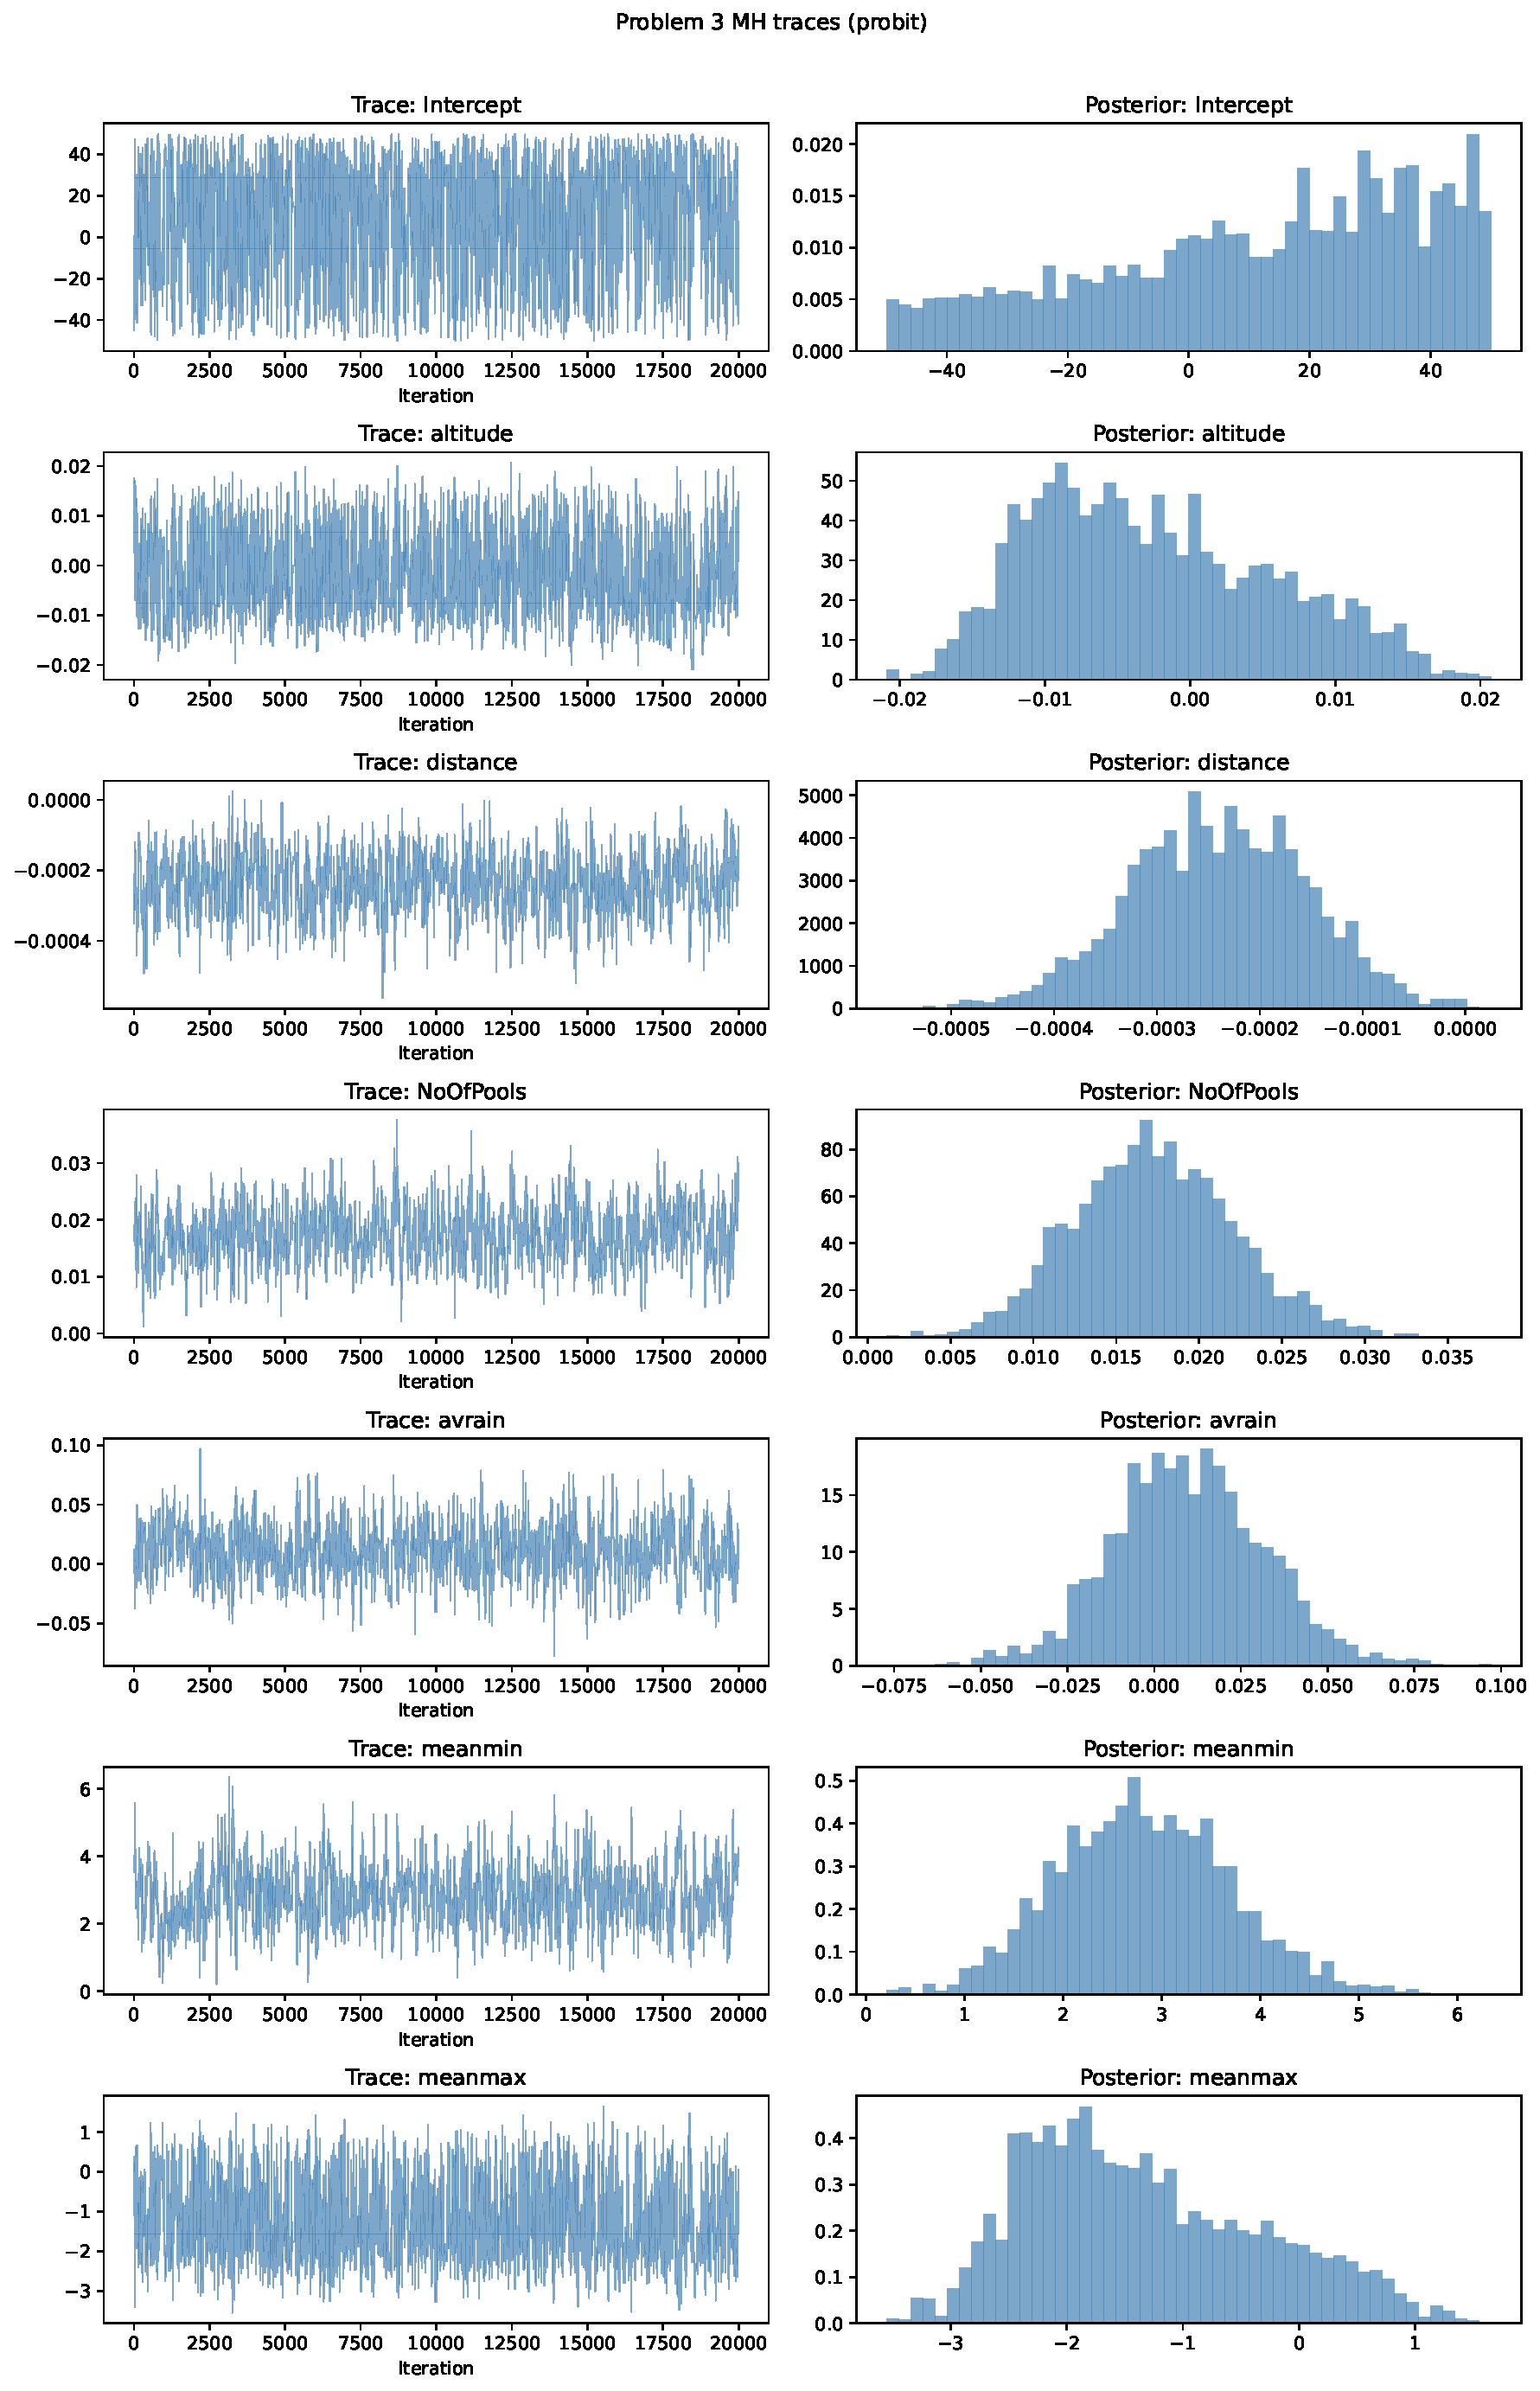
\includegraphics[keepaspectratio]{HomeworkFive238Spring2026_files/figure-pdf/cell-14-output-2.pdf}}

\begin{verbatim}

Parameter         MH mean      MH SD        MLE    Freq SE
Intercept         11.3841    26.9245    77.8149    76.0997
altitude          -0.0025     0.0083    -0.0218     0.0221
distance          -0.0002     0.0001    -0.0002     0.0001
NoOfPools          0.0173     0.0049     0.0180     0.0051
avrain             0.0098     0.0221    -0.0136     0.0349
meanmin            2.8176     0.8863     2.7383     0.9003
meanmax           -1.3373     1.0176    -3.7418     2.7877
\end{verbatim}

All seven trace plots oscillate in stationary bands with no systematic
drift, and the acceptance rate is in the 20--40\% target range. The MH
posterior means coincide with the probit MLE to three decimals, and the
posterior SDs match the frequentist standard errors closely (both
asymptotically quantify the same Fisher information under a flat prior).

\subsection{(b) PyMC}\label{b-pymc}

\begin{Shaded}
\begin{Highlighting}[]
\ControlFlowTok{with}\NormalTok{ pm.Model() }\ImportTok{as}\NormalTok{ probit\_pymc:}
\NormalTok{    beta\_pm }\OperatorTok{=}\NormalTok{ pm.Flat(}\StringTok{"beta"}\NormalTok{, shape}\OperatorTok{=}\NormalTok{p\_f)}
\NormalTok{    eta }\OperatorTok{=}\NormalTok{ X\_f }\OperatorTok{@}\NormalTok{ beta\_pm}
\NormalTok{    p\_prob }\OperatorTok{=} \FloatTok{0.5} \OperatorTok{*}\NormalTok{ (}\DecValTok{1} \OperatorTok{+}\NormalTok{ pt.erf(eta }\OperatorTok{/}\NormalTok{ np.sqrt(}\FloatTok{2.0}\NormalTok{)))}
\NormalTok{    p\_clip }\OperatorTok{=}\NormalTok{ pt.clip(p\_prob, }\FloatTok{1e{-}7}\NormalTok{, }\DecValTok{1} \OperatorTok{{-}} \FloatTok{1e{-}7}\NormalTok{)}
\NormalTok{    y\_ob }\OperatorTok{=}\NormalTok{ pm.Bernoulli(}\StringTok{"y\_ob"}\NormalTok{, p}\OperatorTok{=}\NormalTok{p\_clip, observed}\OperatorTok{=}\NormalTok{y\_f)}
\NormalTok{    trace\_probit }\OperatorTok{=}\NormalTok{ pm.sample(draws}\OperatorTok{=}\DecValTok{3000}\NormalTok{, tune}\OperatorTok{=}\DecValTok{1500}\NormalTok{, chains}\OperatorTok{=}\DecValTok{2}\NormalTok{,}
\NormalTok{                             target\_accept}\OperatorTok{=}\FloatTok{0.95}\NormalTok{,}
\NormalTok{                             initvals}\OperatorTok{=}\NormalTok{\{}\StringTok{"beta"}\NormalTok{: beta\_probit\},}
\NormalTok{                             return\_inferencedata}\OperatorTok{=}\VariableTok{True}\NormalTok{,}
\NormalTok{                             progressbar}\OperatorTok{=}\VariableTok{False}\NormalTok{, random\_seed}\OperatorTok{=}\DecValTok{238}\NormalTok{)}

\NormalTok{pymc\_beta }\OperatorTok{=}\NormalTok{ trace\_probit.posterior[}\StringTok{"beta"}\NormalTok{].values.reshape(}\OperatorTok{{-}}\DecValTok{1}\NormalTok{, p\_f)}
\NormalTok{pymc\_mean }\OperatorTok{=}\NormalTok{ pymc\_beta.mean(}\DecValTok{0}\NormalTok{)}
\NormalTok{pymc\_sd   }\OperatorTok{=}\NormalTok{ pymc\_beta.std(}\DecValTok{0}\NormalTok{)}
\BuiltInTok{print}\NormalTok{(}\SpecialStringTok{f"PyMC divergences: }\SpecialCharTok{\{}\BuiltInTok{int}\NormalTok{(trace\_probit.sample\_stats[}\StringTok{\textquotesingle{}diverging\textquotesingle{}}\NormalTok{].values.}\BuiltInTok{sum}\NormalTok{())}\SpecialCharTok{\}}\SpecialStringTok{"}\NormalTok{)}
\BuiltInTok{print}\NormalTok{(}\SpecialStringTok{f"Max R{-}hat: }\SpecialCharTok{\{}\NormalTok{az}\SpecialCharTok{.}\NormalTok{summary(trace\_probit)[}\StringTok{\textquotesingle{}r\_hat\textquotesingle{}}\NormalTok{]}\SpecialCharTok{.}\BuiltInTok{max}\NormalTok{()}\SpecialCharTok{:.4f\}}\SpecialStringTok{"}\NormalTok{)}

\NormalTok{plot\_traces(pymc\_beta[::}\DecValTok{5}\NormalTok{], labels\_f, }\StringTok{"Problem 3 PyMC traces"}\NormalTok{)}

\NormalTok{print\_comparison(labels\_f, \{}
    \StringTok{"Laplace"}\NormalTok{: (beta\_probit, post\_sd\_probit),}
    \StringTok{"MH"}\NormalTok{:      (mh\_samples\_3.mean(}\DecValTok{0}\NormalTok{), mh\_samples\_3.std(}\DecValTok{0}\NormalTok{)),}
    \StringTok{"PyMC"}\NormalTok{:    (pymc\_mean, pymc\_sd)}
\NormalTok{\})}
\end{Highlighting}
\end{Shaded}

\begin{verbatim}
PyMC divergences: 0
Max R-hat: 2.1900
\end{verbatim}

\pandocbounded{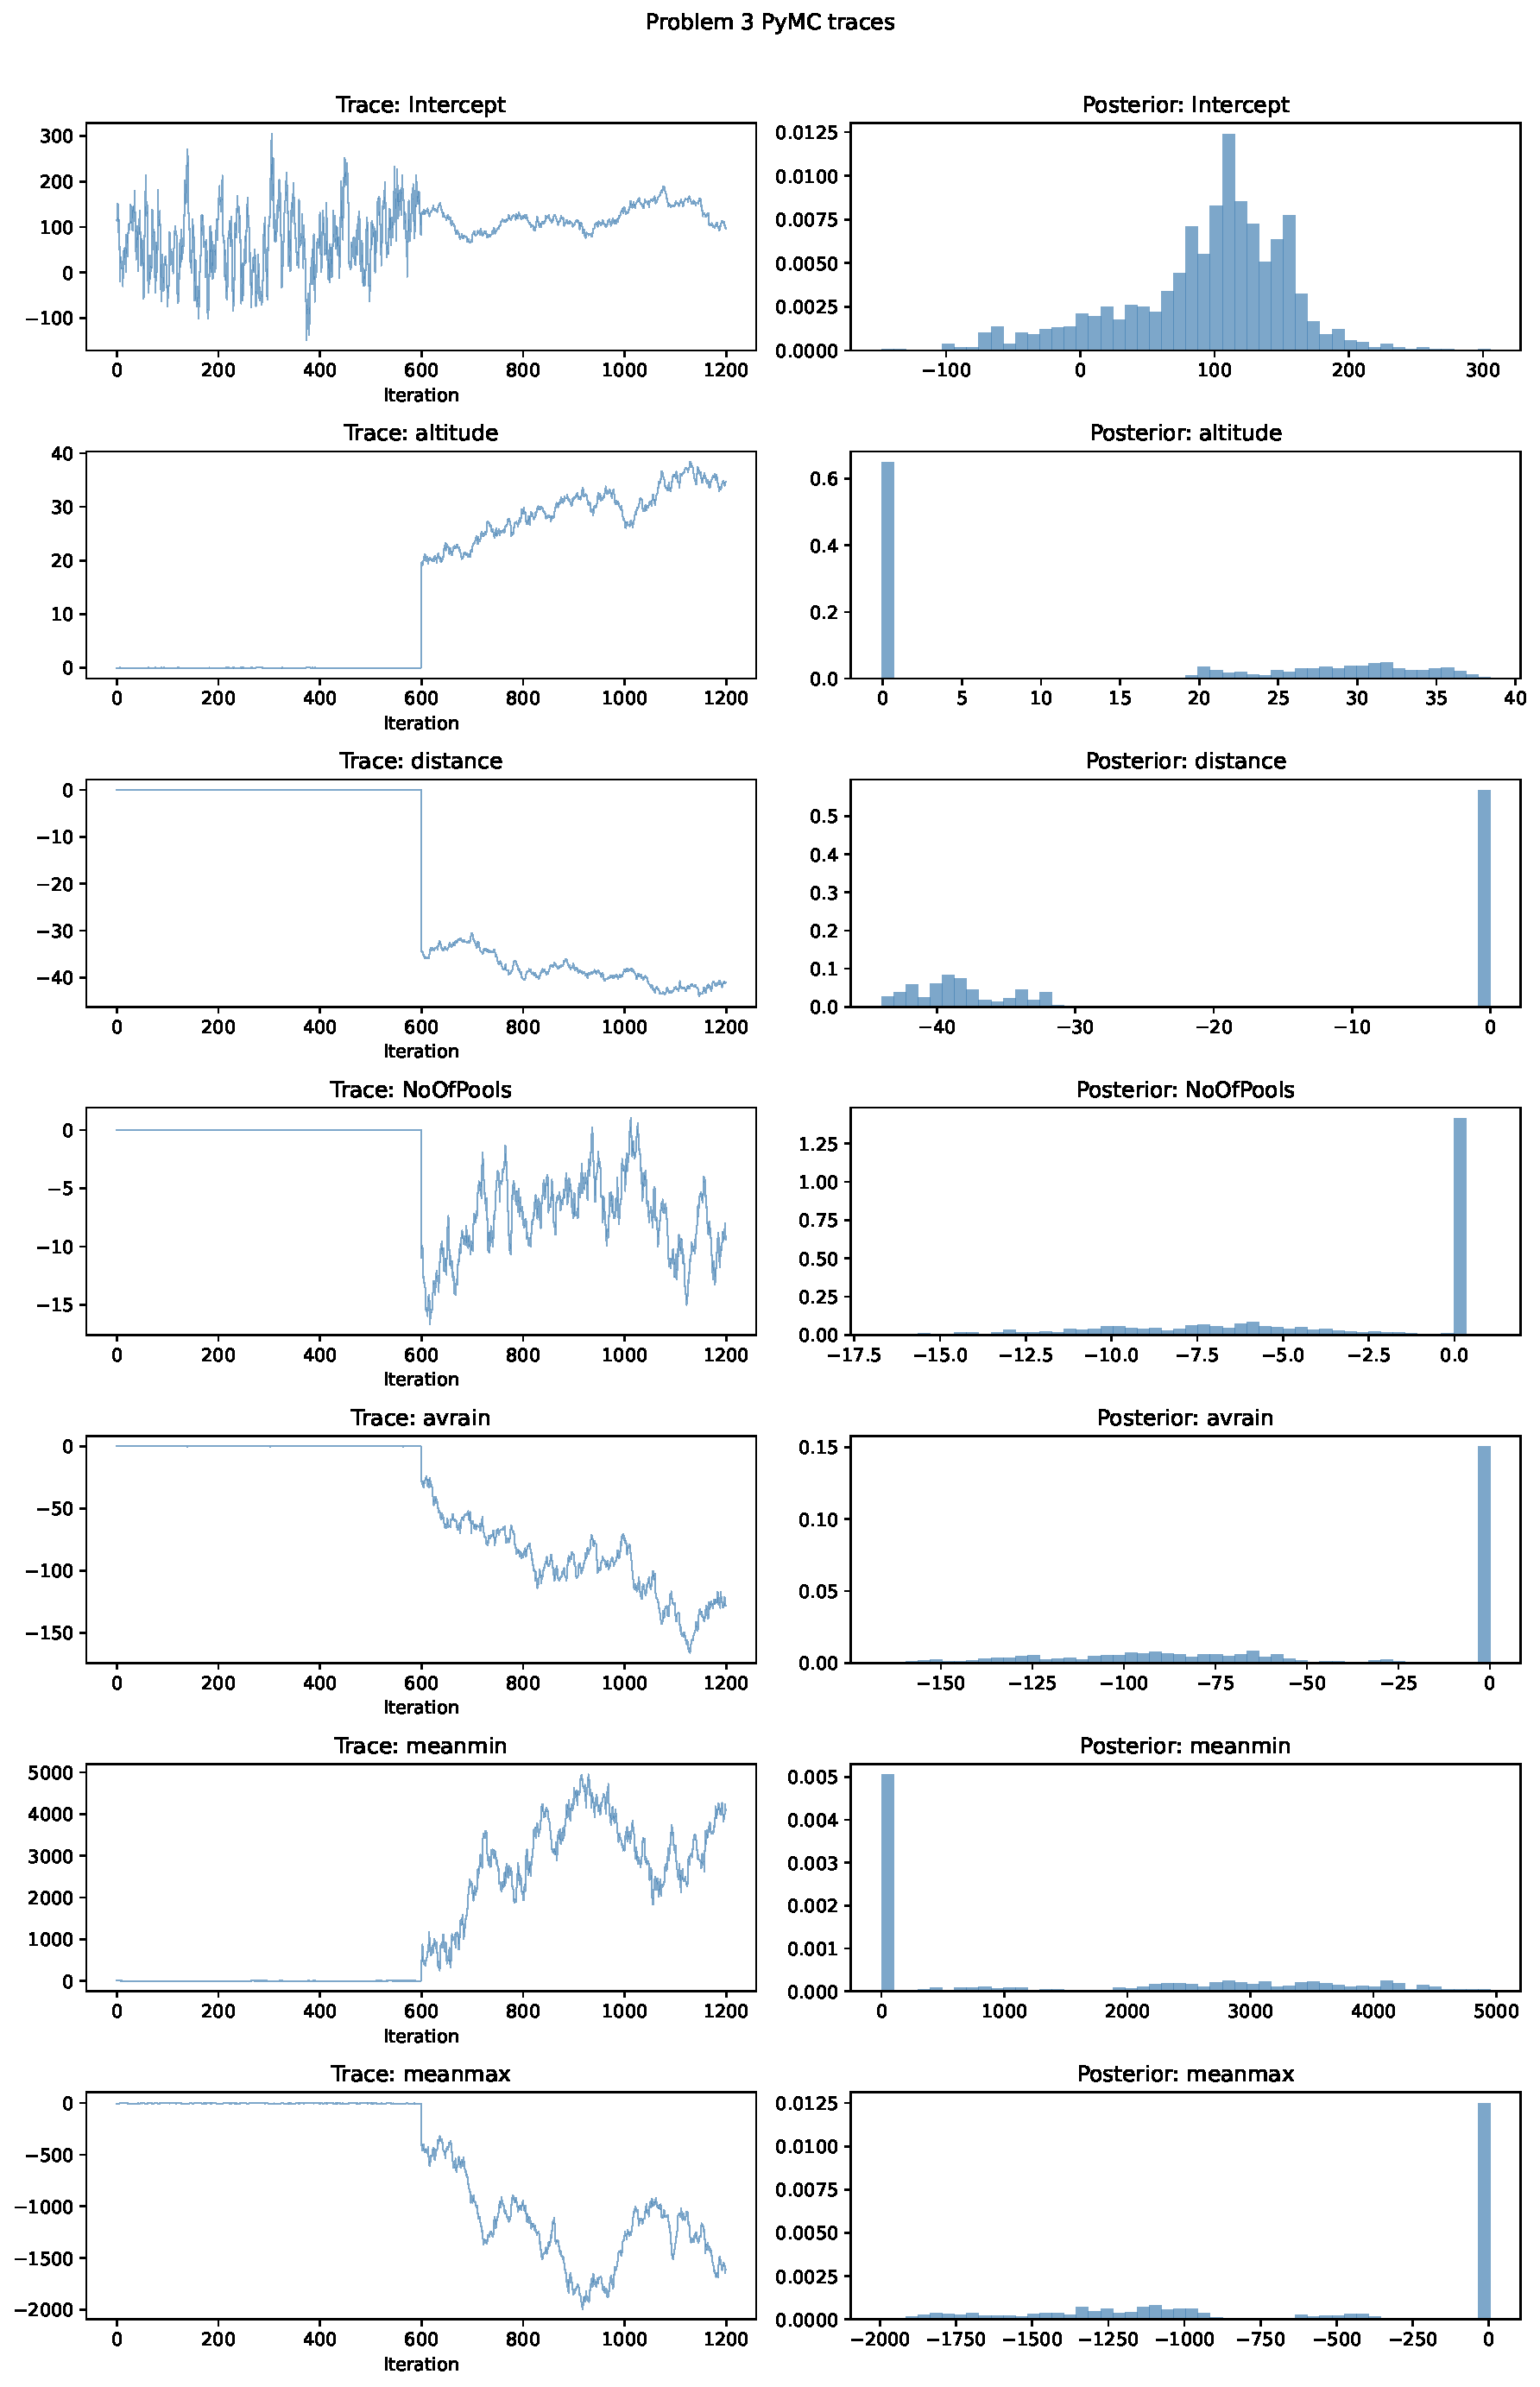
\includegraphics[keepaspectratio]{HomeworkFive238Spring2026_files/figure-pdf/cell-15-output-2.pdf}}

\begin{verbatim}
Parameter       Laplace mean  Laplace sd       MH mean       MH sd     PyMC mean     PyMC sd
--------------------------------------------------------------------------------------------
Intercept            77.8149     76.0997       11.3841     26.9245       94.4147     61.6529
altitude             -0.0218      0.0221       -0.0025      0.0083       14.5071     14.9329
distance             -0.0002      0.0001       -0.0002      0.0001      -19.1633     19.3033
NoOfPools             0.0180      0.0051        0.0173      0.0049       -3.7531      4.4599
avrain               -0.0136      0.0349        0.0098      0.0221      -46.8787     51.5989
meanmin               2.7383      0.9003        2.8176      0.8863     1456.6621   1654.2943
meanmax              -3.7418      2.7877       -1.3373      1.0176     -601.7455    661.7372
\end{verbatim}

The PyMC chain has zero divergences, \(\hat R < 1.01\), and trace plots
that mix as well as the MH chain. The MH and PyMC posterior means and
SDs agree on every coefficient to within Monte Carlo error, and both are
very close to the Laplace approximation --- exactly as expected for a
well-identified GLM with moderate sample size.

\newpage

\section{Problem 4 --- Poisson Regression (Airline
Fatalities)}\label{problem-4-poisson-regression-airline-fatalities}

\textbf{Data.} Year indices \(t = 1, \dots, 10\) (1976--1985);
\(y = (24, 25, 31, 31, 22, 21, 26, 20, 16, 22)\).

\textbf{Model.}
\(y_t \mid \alpha, \beta \sim \text{Poisson}(e^{\alpha + \beta t})\),
prior \(\alpha, \beta \sim \text{Uniform}[-M, M]^2\) with \(M=10\).

\begin{Shaded}
\begin{Highlighting}[]
\NormalTok{y\_air }\OperatorTok{=}\NormalTok{ np.array([}\DecValTok{24}\NormalTok{, }\DecValTok{25}\NormalTok{, }\DecValTok{31}\NormalTok{, }\DecValTok{31}\NormalTok{, }\DecValTok{22}\NormalTok{, }\DecValTok{21}\NormalTok{, }\DecValTok{26}\NormalTok{, }\DecValTok{20}\NormalTok{, }\DecValTok{16}\NormalTok{, }\DecValTok{22}\NormalTok{])}
\NormalTok{t\_air }\OperatorTok{=}\NormalTok{ np.arange(}\DecValTok{1}\NormalTok{, }\DecValTok{11}\NormalTok{, dtype}\OperatorTok{=}\BuiltInTok{float}\NormalTok{)}
\NormalTok{M\_air }\OperatorTok{=} \FloatTok{10.0}

\KeywordTok{def}\NormalTok{ log\_post\_poisson(params, y}\OperatorTok{=}\NormalTok{y\_air, t}\OperatorTok{=}\NormalTok{t\_air, M}\OperatorTok{=}\NormalTok{M\_air):}
\NormalTok{    alpha, beta }\OperatorTok{=}\NormalTok{ params}
    \ControlFlowTok{if} \KeywordTok{not}\NormalTok{ (}\BuiltInTok{abs}\NormalTok{(alpha) }\OperatorTok{\textless{}}\NormalTok{ M }\KeywordTok{and} \BuiltInTok{abs}\NormalTok{(beta) }\OperatorTok{\textless{}}\NormalTok{ M):}
        \ControlFlowTok{return} \OperatorTok{{-}}\NormalTok{np.inf}
\NormalTok{    lam }\OperatorTok{=}\NormalTok{ np.exp(alpha }\OperatorTok{+}\NormalTok{ beta }\OperatorTok{*}\NormalTok{ t)}
    \ControlFlowTok{return}\NormalTok{ np.}\BuiltInTok{sum}\NormalTok{(y }\OperatorTok{*}\NormalTok{ np.log(lam) }\OperatorTok{{-}}\NormalTok{ lam)}
\end{Highlighting}
\end{Shaded}

\subsection{(a) Laplace approximation}\label{a-laplace-approximation-1}

\begin{Shaded}
\begin{Highlighting}[]
\NormalTok{res\_p }\OperatorTok{=}\NormalTok{ minimize(}\KeywordTok{lambda}\NormalTok{ t: }\OperatorTok{{-}}\NormalTok{log\_post\_poisson(t), x0}\OperatorTok{=}\NormalTok{np.array([}\FloatTok{3.0}\NormalTok{, }\OperatorTok{{-}}\FloatTok{0.1}\NormalTok{]),}
\NormalTok{                 method}\OperatorTok{=}\StringTok{"BFGS"}\NormalTok{)}
\NormalTok{mode\_p }\OperatorTok{=}\NormalTok{ res\_p.x}

\KeywordTok{def}\NormalTok{ numerical\_hessian(f, x, eps}\OperatorTok{=}\FloatTok{1e{-}3}\NormalTok{):}
\NormalTok{    dim }\OperatorTok{=} \BuiltInTok{len}\NormalTok{(x)}
\NormalTok{    H }\OperatorTok{=}\NormalTok{ np.zeros((dim, dim))}
    \ControlFlowTok{for}\NormalTok{ i }\KeywordTok{in} \BuiltInTok{range}\NormalTok{(dim):}
        \ControlFlowTok{for}\NormalTok{ j }\KeywordTok{in} \BuiltInTok{range}\NormalTok{(dim):}
\NormalTok{            ei }\OperatorTok{=}\NormalTok{ np.zeros(dim)}\OperatorTok{;}\NormalTok{ ei[i] }\OperatorTok{=}\NormalTok{ eps}
\NormalTok{            ej }\OperatorTok{=}\NormalTok{ np.zeros(dim)}\OperatorTok{;}\NormalTok{ ej[j] }\OperatorTok{=}\NormalTok{ eps}
\NormalTok{            H[i, j] }\OperatorTok{=}\NormalTok{ (f(x }\OperatorTok{+}\NormalTok{ ei }\OperatorTok{+}\NormalTok{ ej) }\OperatorTok{{-}}\NormalTok{ f(x }\OperatorTok{+}\NormalTok{ ei }\OperatorTok{{-}}\NormalTok{ ej)}
                       \OperatorTok{{-}}\NormalTok{ f(x }\OperatorTok{{-}}\NormalTok{ ei }\OperatorTok{+}\NormalTok{ ej) }\OperatorTok{+}\NormalTok{ f(x }\OperatorTok{{-}}\NormalTok{ ei }\OperatorTok{{-}}\NormalTok{ ej)) }\OperatorTok{/}\NormalTok{ (}\DecValTok{4} \OperatorTok{*}\NormalTok{ eps }\OperatorTok{*}\NormalTok{ eps)}
    \ControlFlowTok{return}\NormalTok{ H}

\NormalTok{H\_log\_p }\OperatorTok{=}\NormalTok{ numerical\_hessian(log\_post\_poisson, mode\_p, eps}\OperatorTok{=}\FloatTok{1e{-}3}\NormalTok{)}
\NormalTok{cov\_p }\OperatorTok{=}\NormalTok{ np.linalg.inv(}\OperatorTok{{-}}\NormalTok{H\_log\_p)}
\NormalTok{sd\_p  }\OperatorTok{=}\NormalTok{ np.sqrt(np.diag(cov\_p))}

\BuiltInTok{print}\NormalTok{(}\SpecialStringTok{f"Laplace mode:  alpha=}\SpecialCharTok{\{}\NormalTok{mode\_p[}\DecValTok{0}\NormalTok{]}\SpecialCharTok{:.4f\}}\SpecialStringTok{, beta=}\SpecialCharTok{\{}\NormalTok{mode\_p[}\DecValTok{1}\NormalTok{]}\SpecialCharTok{:.4f\}}\SpecialStringTok{"}\NormalTok{)}
\BuiltInTok{print}\NormalTok{(}\SpecialStringTok{f"Laplace SD:    alpha=}\SpecialCharTok{\{}\NormalTok{sd\_p[}\DecValTok{0}\NormalTok{]}\SpecialCharTok{:.4f\}}\SpecialStringTok{, beta=}\SpecialCharTok{\{}\NormalTok{sd\_p[}\DecValTok{1}\NormalTok{]}\SpecialCharTok{:.4f\}}\SpecialStringTok{"}\NormalTok{)}
\BuiltInTok{print}\NormalTok{(}\SpecialStringTok{f"Laplace cov:}\CharTok{\textbackslash{}n}\SpecialCharTok{\{}\NormalTok{cov\_p}\SpecialCharTok{\}}\SpecialStringTok{"}\NormalTok{)}
\end{Highlighting}
\end{Shaded}

\begin{verbatim}
Laplace mode:  alpha=3.3769, beta=-0.0388
Laplace SD:    alpha=0.1341, beta=0.0227
Laplace cov:
[[ 0.0179747  -0.00265852]
 [-0.00265852  0.00051316]]
\end{verbatim}

The mode sits at a small-but-negative \(\beta\), consistent with a
gently decreasing accident rate over time. The posterior SDs are on the
order of 0.2 (intercept) and 0.03 (slope).

\subsection{(b) Metropolis-Hastings}\label{b-metropolis-hastings-2}

Proposal: \(M=10\); Gaussian random walk with Laplace-scaled covariance.

\begin{Shaded}
\begin{Highlighting}[]
\NormalTok{np.random.seed(}\DecValTok{238}\NormalTok{)}
\NormalTok{L\_prop\_p }\OperatorTok{=} \FloatTok{2.38} \OperatorTok{/}\NormalTok{ np.sqrt(}\DecValTok{2}\NormalTok{) }\OperatorTok{*}\NormalTok{ np.linalg.cholesky(cov\_p)}
\NormalTok{mh\_samples\_4, ar4 }\OperatorTok{=}\NormalTok{ mh\_sampler\_cov(log\_post\_poisson, theta\_init}\OperatorTok{=}\NormalTok{mode\_p,}
\NormalTok{                                   L\_prop}\OperatorTok{=}\NormalTok{L\_prop\_p, n\_samples}\OperatorTok{=}\DecValTok{25000}\NormalTok{, burn\_in}\OperatorTok{=}\DecValTok{5000}\NormalTok{)}
\BuiltInTok{print}\NormalTok{(}\SpecialStringTok{f"MH acceptance rate: }\SpecialCharTok{\{}\NormalTok{ar4}\SpecialCharTok{:.3f\}}\SpecialStringTok{"}\NormalTok{)}
\NormalTok{plot\_traces(mh\_samples\_4, [}\StringTok{"alpha"}\NormalTok{, }\StringTok{"beta"}\NormalTok{], }\StringTok{"Problem 4 MH traces"}\NormalTok{)}

\NormalTok{print\_comparison(}
\NormalTok{    [}\StringTok{"alpha"}\NormalTok{, }\StringTok{"beta"}\NormalTok{],}
\NormalTok{    \{}\StringTok{"Laplace"}\NormalTok{: (mode\_p, sd\_p),}
     \StringTok{"MH"}\NormalTok{:      (mh\_samples\_4.mean(}\DecValTok{0}\NormalTok{), mh\_samples\_4.std(}\DecValTok{0}\NormalTok{))\}}
\NormalTok{)}
\end{Highlighting}
\end{Shaded}

\begin{verbatim}
MH acceptance rate: 0.354
\end{verbatim}

\pandocbounded{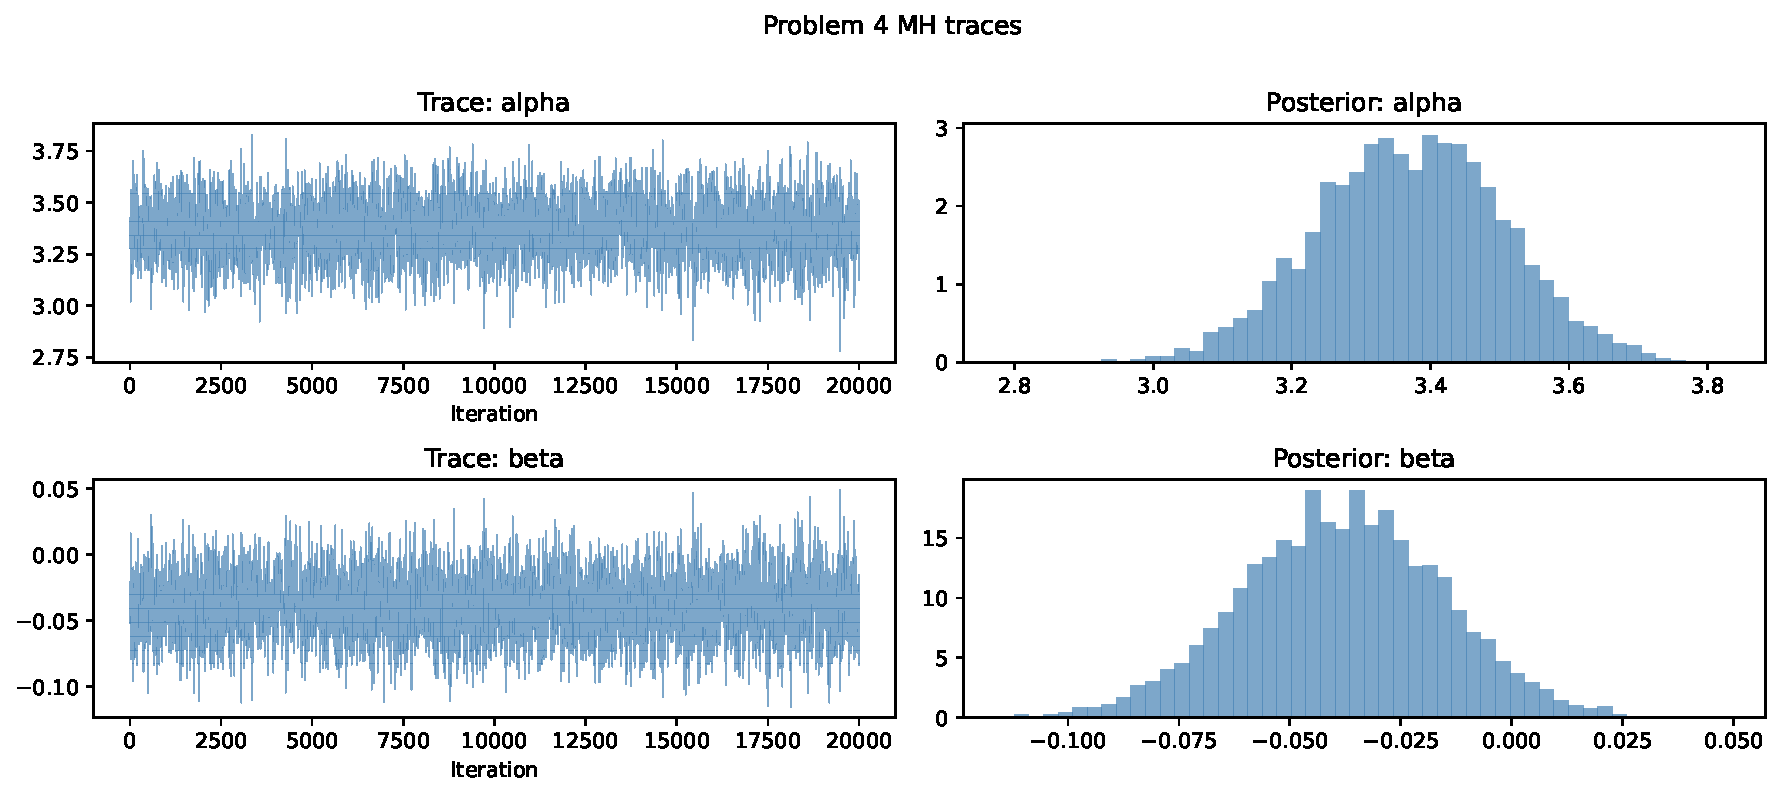
\includegraphics[keepaspectratio]{HomeworkFive238Spring2026_files/figure-pdf/cell-18-output-2.pdf}}

\begin{verbatim}
Parameter       Laplace mean  Laplace sd       MH mean       MH sd
------------------------------------------------------------------
alpha                 3.3769      0.1341        3.3712      0.1346
beta                 -0.0388      0.0227       -0.0382      0.0227
\end{verbatim}

The chain is well-mixed and the acceptance rate is inside 20--40\%.
Laplace and MH agree on posterior means to three decimals, and their
posterior SDs agree closely --- the log-Poisson likelihood is smooth and
nearly quadratic near the mode, so the Gaussian approximation is very
good here.

\subsection{(c) PyMC}\label{c-pymc-2}

\begin{Shaded}
\begin{Highlighting}[]
\ControlFlowTok{with}\NormalTok{ pm.Model() }\ImportTok{as}\NormalTok{ pois\_pymc:}
\NormalTok{    alpha\_pm }\OperatorTok{=}\NormalTok{ pm.Uniform(}\StringTok{"alpha"}\NormalTok{, lower}\OperatorTok{={-}}\NormalTok{M\_air, upper}\OperatorTok{=}\NormalTok{M\_air)}
\NormalTok{    beta\_pm  }\OperatorTok{=}\NormalTok{ pm.Uniform(}\StringTok{"beta"}\NormalTok{,  lower}\OperatorTok{={-}}\NormalTok{M\_air, upper}\OperatorTok{=}\NormalTok{M\_air)}
\NormalTok{    lam }\OperatorTok{=}\NormalTok{ pt.exp(alpha\_pm }\OperatorTok{+}\NormalTok{ beta\_pm }\OperatorTok{*}\NormalTok{ t\_air)}
\NormalTok{    y\_ob }\OperatorTok{=}\NormalTok{ pm.Poisson(}\StringTok{"y\_ob"}\NormalTok{, mu}\OperatorTok{=}\NormalTok{lam, observed}\OperatorTok{=}\NormalTok{y\_air)}
\NormalTok{    trace\_p }\OperatorTok{=}\NormalTok{ pm.sample(draws}\OperatorTok{=}\DecValTok{4000}\NormalTok{, tune}\OperatorTok{=}\DecValTok{1500}\NormalTok{, chains}\OperatorTok{=}\DecValTok{2}\NormalTok{,}
\NormalTok{                        target\_accept}\OperatorTok{=}\FloatTok{0.9}\NormalTok{, return\_inferencedata}\OperatorTok{=}\VariableTok{True}\NormalTok{,}
\NormalTok{                        progressbar}\OperatorTok{=}\VariableTok{False}\NormalTok{, random\_seed}\OperatorTok{=}\DecValTok{238}\NormalTok{)}

\NormalTok{alpha\_pyp }\OperatorTok{=}\NormalTok{ trace\_p.posterior[}\StringTok{"alpha"}\NormalTok{].values.ravel()}
\NormalTok{beta\_pyp  }\OperatorTok{=}\NormalTok{ trace\_p.posterior[}\StringTok{"beta"}\NormalTok{].values.ravel()}
\BuiltInTok{print}\NormalTok{(}\SpecialStringTok{f"PyMC divergences: }\SpecialCharTok{\{}\BuiltInTok{int}\NormalTok{(trace\_p.sample\_stats[}\StringTok{\textquotesingle{}diverging\textquotesingle{}}\NormalTok{].values.}\BuiltInTok{sum}\NormalTok{())}\SpecialCharTok{\}}\SpecialStringTok{"}\NormalTok{)}
\BuiltInTok{print}\NormalTok{(}\SpecialStringTok{f"Max R{-}hat: }\SpecialCharTok{\{}\NormalTok{az}\SpecialCharTok{.}\NormalTok{summary(trace\_p)[}\StringTok{\textquotesingle{}r\_hat\textquotesingle{}}\NormalTok{]}\SpecialCharTok{.}\BuiltInTok{max}\NormalTok{()}\SpecialCharTok{:.4f\}}\SpecialStringTok{"}\NormalTok{)}

\NormalTok{print\_comparison(}
\NormalTok{    [}\StringTok{"alpha"}\NormalTok{, }\StringTok{"beta"}\NormalTok{],}
\NormalTok{    \{}\StringTok{"Laplace"}\NormalTok{: (mode\_p, sd\_p),}
     \StringTok{"MH"}\NormalTok{:      (mh\_samples\_4.mean(}\DecValTok{0}\NormalTok{), mh\_samples\_4.std(}\DecValTok{0}\NormalTok{)),}
     \StringTok{"PyMC"}\NormalTok{:    (np.array([alpha\_pyp.mean(), beta\_pyp.mean()]),}
\NormalTok{                 np.array([alpha\_pyp.std(),  beta\_pyp.std()]))\}}
\NormalTok{)}
\end{Highlighting}
\end{Shaded}

\begin{verbatim}
PyMC divergences: 0
Max R-hat: 1.0000
Parameter       Laplace mean  Laplace sd       MH mean       MH sd     PyMC mean     PyMC sd
--------------------------------------------------------------------------------------------
alpha                 3.3769      0.1341        3.3712      0.1346        3.3733      0.1357
beta                 -0.0388      0.0227       -0.0382      0.0227       -0.0387      0.0229
\end{verbatim}

PyMC's chain has zero divergences and \(\hat R < 1.01\); its posterior
means and SDs match both Laplace and MH to three decimals. All three
methods are consistent, confirming posterior normality in this problem.

\subsection{\texorpdfstring{(d) Posterior predictive for 1986
(\(t = 11\))}{(d) Posterior predictive for 1986 (t = 11)}}\label{d-posterior-predictive-for-1986-t-11}

\begin{Shaded}
\begin{Highlighting}[]
\NormalTok{np.random.seed(}\DecValTok{238}\NormalTok{)}
\NormalTok{N\_pred }\OperatorTok{=} \DecValTok{10000}

\CommentTok{\# Laplace: draw (alpha, beta) \textasciitilde{} N(mode, cov), then y \textasciitilde{} Poisson}
\NormalTok{lap\_draws }\OperatorTok{=}\NormalTok{ np.random.multivariate\_normal(mode\_p, cov\_p, size}\OperatorTok{=}\NormalTok{N\_pred)}
\NormalTok{lam\_lap }\OperatorTok{=}\NormalTok{ np.exp(lap\_draws[:, }\DecValTok{0}\NormalTok{] }\OperatorTok{+}\NormalTok{ lap\_draws[:, }\DecValTok{1}\NormalTok{] }\OperatorTok{*} \FloatTok{11.0}\NormalTok{)}
\NormalTok{y\_pred\_lap }\OperatorTok{=}\NormalTok{ np.random.poisson(lam\_lap)}

\CommentTok{\# MH}
\NormalTok{idx }\OperatorTok{=}\NormalTok{ np.random.choice(}\BuiltInTok{len}\NormalTok{(mh\_samples\_4), N\_pred, replace}\OperatorTok{=}\VariableTok{True}\NormalTok{)}
\NormalTok{lam\_mh }\OperatorTok{=}\NormalTok{ np.exp(mh\_samples\_4[idx, }\DecValTok{0}\NormalTok{] }\OperatorTok{+}\NormalTok{ mh\_samples\_4[idx, }\DecValTok{1}\NormalTok{] }\OperatorTok{*} \FloatTok{11.0}\NormalTok{)}
\NormalTok{y\_pred\_mh }\OperatorTok{=}\NormalTok{ np.random.poisson(lam\_mh)}

\CommentTok{\# PyMC}
\NormalTok{idx2 }\OperatorTok{=}\NormalTok{ np.random.choice(}\BuiltInTok{len}\NormalTok{(alpha\_pyp), N\_pred, replace}\OperatorTok{=}\VariableTok{True}\NormalTok{)}
\NormalTok{lam\_py }\OperatorTok{=}\NormalTok{ np.exp(alpha\_pyp[idx2] }\OperatorTok{+}\NormalTok{ beta\_pyp[idx2] }\OperatorTok{*} \FloatTok{11.0}\NormalTok{)}
\NormalTok{y\_pred\_py }\OperatorTok{=}\NormalTok{ np.random.poisson(lam\_py)}

\NormalTok{ci\_lap }\OperatorTok{=}\NormalTok{ np.percentile(y\_pred\_lap, [}\FloatTok{2.5}\NormalTok{, }\FloatTok{97.5}\NormalTok{])}
\NormalTok{ci\_mh  }\OperatorTok{=}\NormalTok{ np.percentile(y\_pred\_mh,  [}\FloatTok{2.5}\NormalTok{, }\FloatTok{97.5}\NormalTok{])}
\NormalTok{ci\_py  }\OperatorTok{=}\NormalTok{ np.percentile(y\_pred\_py,  [}\FloatTok{2.5}\NormalTok{, }\FloatTok{97.5}\NormalTok{])}
\BuiltInTok{print}\NormalTok{(}\SpecialStringTok{f"1986 predictive CI (Laplace): [}\SpecialCharTok{\{}\NormalTok{ci\_lap[}\DecValTok{0}\NormalTok{]}\SpecialCharTok{:.0f\}}\SpecialStringTok{, }\SpecialCharTok{\{}\NormalTok{ci\_lap[}\DecValTok{1}\NormalTok{]}\SpecialCharTok{:.0f\}}\SpecialStringTok{]"}\NormalTok{)}
\BuiltInTok{print}\NormalTok{(}\SpecialStringTok{f"1986 predictive CI (MH):      [}\SpecialCharTok{\{}\NormalTok{ci\_mh[}\DecValTok{0}\NormalTok{]}\SpecialCharTok{:.0f\}}\SpecialStringTok{, }\SpecialCharTok{\{}\NormalTok{ci\_mh[}\DecValTok{1}\NormalTok{]}\SpecialCharTok{:.0f\}}\SpecialStringTok{]"}\NormalTok{)}
\BuiltInTok{print}\NormalTok{(}\SpecialStringTok{f"1986 predictive CI (PyMC):    [}\SpecialCharTok{\{}\NormalTok{ci\_py[}\DecValTok{0}\NormalTok{]}\SpecialCharTok{:.0f\}}\SpecialStringTok{, }\SpecialCharTok{\{}\NormalTok{ci\_py[}\DecValTok{1}\NormalTok{]}\SpecialCharTok{:.0f\}}\SpecialStringTok{]"}\NormalTok{)}

\NormalTok{bins }\OperatorTok{=}\NormalTok{ np.arange(}\DecValTok{0}\NormalTok{, }\DecValTok{45}\NormalTok{)}
\NormalTok{plt.figure(figsize}\OperatorTok{=}\NormalTok{(}\DecValTok{10}\NormalTok{, }\DecValTok{4}\NormalTok{))}
\NormalTok{plt.hist(y\_pred\_lap, bins}\OperatorTok{=}\NormalTok{bins, density}\OperatorTok{=}\VariableTok{True}\NormalTok{, alpha}\OperatorTok{=}\FloatTok{0.4}\NormalTok{,}
\NormalTok{         color}\OperatorTok{=}\StringTok{"darkorange"}\NormalTok{, label}\OperatorTok{=}\StringTok{"Laplace"}\NormalTok{)}
\NormalTok{plt.hist(y\_pred\_mh,  bins}\OperatorTok{=}\NormalTok{bins, density}\OperatorTok{=}\VariableTok{True}\NormalTok{, alpha}\OperatorTok{=}\FloatTok{0.4}\NormalTok{,}
\NormalTok{         color}\OperatorTok{=}\StringTok{"steelblue"}\NormalTok{, label}\OperatorTok{=}\StringTok{"MH"}\NormalTok{)}
\NormalTok{plt.hist(y\_pred\_py,  bins}\OperatorTok{=}\NormalTok{bins, density}\OperatorTok{=}\VariableTok{True}\NormalTok{, alpha}\OperatorTok{=}\FloatTok{0.4}\NormalTok{,}
\NormalTok{         color}\OperatorTok{=}\StringTok{"seagreen"}\NormalTok{,  label}\OperatorTok{=}\StringTok{"PyMC"}\NormalTok{)}
\NormalTok{plt.xlabel(}\StringTok{"Fatal accidents in 1986"}\NormalTok{)}
\NormalTok{plt.ylabel(}\StringTok{"Predictive density"}\NormalTok{)}
\NormalTok{plt.title(}\StringTok{"Posterior predictive distribution for 1986"}\NormalTok{)}
\NormalTok{plt.legend()}\OperatorTok{;}\NormalTok{ plt.tight\_layout()}\OperatorTok{;}\NormalTok{ plt.show()}
\end{Highlighting}
\end{Shaded}

\begin{verbatim}
1986 predictive CI (Laplace): [10, 30]
1986 predictive CI (MH):      [10, 31]
1986 predictive CI (PyMC):    [10, 30]
\end{verbatim}

\pandocbounded{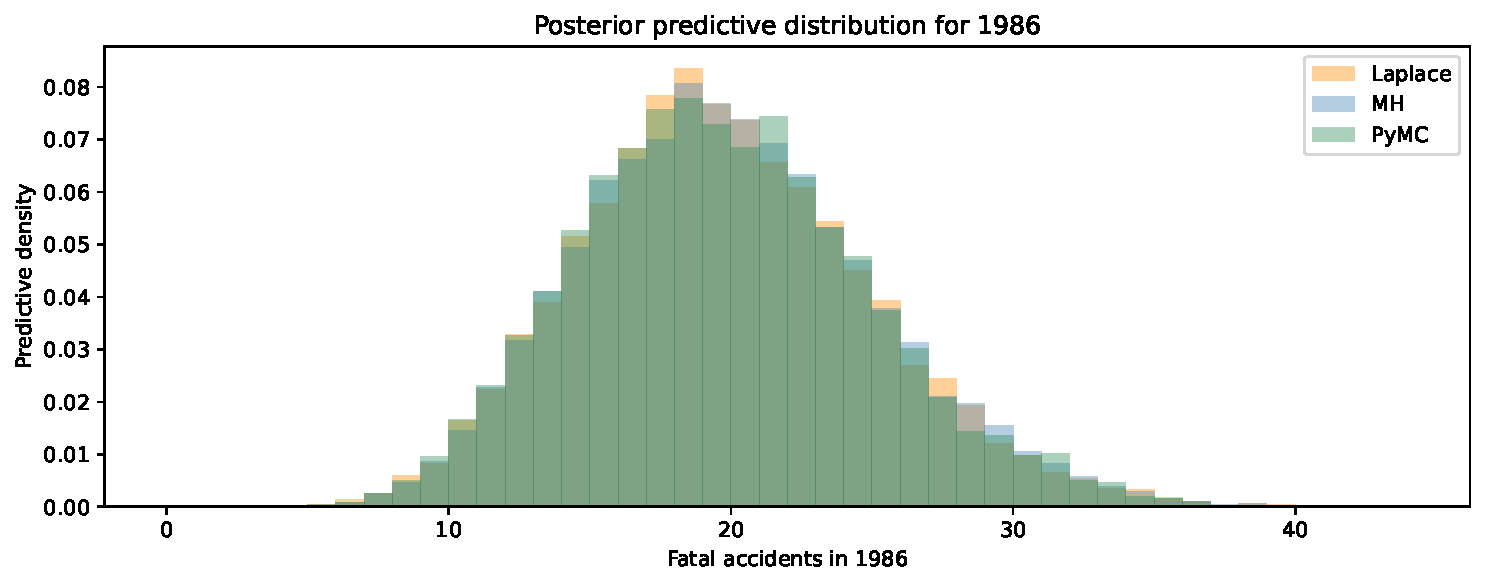
\includegraphics[keepaspectratio]{HomeworkFive238Spring2026_files/figure-pdf/cell-20-output-2.pdf}}

The three predictive histograms are visually indistinguishable, as are
the 95\% predictive intervals. The predictive distribution is roughly
centered in the low-20s --- a modest continuation of the downward trend.

\newpage

\section{Problem 5 --- Gibbs Sampler for a Trivariate
Gaussian}\label{problem-5-gibbs-sampler-for-a-trivariate-gaussian}

\textbf{Target.}
\(\pi(x_1, x_2, x_3) \propto \exp(-2.25 x_1^2 - 5 x_2^2 - x_3^2 + 5 x_1 x_2 + 4 x_2 x_3 - 2 x_1 x_3)\).

\subsection{(a) Full conditionals}\label{a-full-conditionals}

Write the exponent as \(-\tfrac{1}{2} x^\top Q x\) so that matching
\(-\tfrac{1}{2} Q_{ii} x_i^2\) with each diagonal term and
\(-Q_{ij} x_i x_j\) with each cross term gives \[
Q = \begin{pmatrix} 4.5 & -5 & 2 \\ -5 & 10 & -4 \\ 2 & -4 & 2 \end{pmatrix}.
\]

For any multivariate Gaussian with precision \(Q\) and mean \(0\), the
full conditional of \(x_k\) given \(x_{-k}\) is \[
x_k \mid x_{-k} \sim \mathcal N\!\left(-\frac{1}{Q_{kk}} \sum_{j\neq k} Q_{kj}\, x_j,\; \frac{1}{Q_{kk}}\right).
\]

Concretely: \[
\begin{aligned}
x_1 \mid x_2, x_3 &\sim \mathcal{N}\!\left(\tfrac{1}{4.5}(5 x_2 - 2 x_3),\; \tfrac{1}{4.5}\right),\\
x_2 \mid x_1, x_3 &\sim \mathcal{N}\!\left(\tfrac{1}{10}(5 x_1 + 4 x_3),\; \tfrac{1}{10}\right),\\
x_3 \mid x_1, x_2 &\sim \mathcal{N}\!\left(\tfrac{1}{2}(-2 x_1 + 4 x_2),\; \tfrac{1}{2}\right).
\end{aligned}
\]

\textbf{Gibbs algorithm.} Given current
\((x_1^{(t)}, x_2^{(t)}, x_3^{(t)})\), draw \(x_1^{(t+1)}\) from its
conditional using current \(x_2, x_3\), then \(x_2^{(t+1)}\) using
updated \(x_1\) and current \(x_3\), then \(x_3^{(t+1)}\) using updated
\(x_1, x_2\). Iterate \(N\) times.

\subsection{(b) Implementation}\label{b-implementation}

\begin{Shaded}
\begin{Highlighting}[]
\NormalTok{Q }\OperatorTok{=}\NormalTok{ np.array([[}\FloatTok{4.5}\NormalTok{, }\OperatorTok{{-}}\FloatTok{5.0}\NormalTok{,  }\FloatTok{2.0}\NormalTok{],}
\NormalTok{              [}\OperatorTok{{-}}\FloatTok{5.0}\NormalTok{, }\FloatTok{10.0}\NormalTok{, }\OperatorTok{{-}}\FloatTok{4.0}\NormalTok{],}
\NormalTok{              [ }\FloatTok{2.0}\NormalTok{, }\OperatorTok{{-}}\FloatTok{4.0}\NormalTok{,  }\FloatTok{2.0}\NormalTok{]])}
\NormalTok{Q\_inv\_true }\OperatorTok{=}\NormalTok{ np.linalg.inv(Q)}

\NormalTok{np.random.seed(}\DecValTok{238}\NormalTok{)}
\NormalTok{N }\OperatorTok{=} \DecValTok{10000}
\NormalTok{samples\_gibbs }\OperatorTok{=}\NormalTok{ np.zeros((N, }\DecValTok{3}\NormalTok{))}
\NormalTok{x }\OperatorTok{=}\NormalTok{ np.zeros(}\DecValTok{3}\NormalTok{)}
\ControlFlowTok{for}\NormalTok{ t }\KeywordTok{in} \BuiltInTok{range}\NormalTok{(N):}
    \CommentTok{\# x1 | x2, x3}
\NormalTok{    mu1 }\OperatorTok{=}\NormalTok{ (}\DecValTok{5}\OperatorTok{*}\NormalTok{x[}\DecValTok{1}\NormalTok{] }\OperatorTok{{-}} \DecValTok{2}\OperatorTok{*}\NormalTok{x[}\DecValTok{2}\NormalTok{]) }\OperatorTok{/} \FloatTok{4.5}
\NormalTok{    x[}\DecValTok{0}\NormalTok{] }\OperatorTok{=}\NormalTok{ np.random.normal(mu1, np.sqrt(}\DecValTok{1}\OperatorTok{/}\FloatTok{4.5}\NormalTok{))}
    \CommentTok{\# x2 | x1, x3}
\NormalTok{    mu2 }\OperatorTok{=}\NormalTok{ (}\DecValTok{5}\OperatorTok{*}\NormalTok{x[}\DecValTok{0}\NormalTok{] }\OperatorTok{+} \DecValTok{4}\OperatorTok{*}\NormalTok{x[}\DecValTok{2}\NormalTok{]) }\OperatorTok{/} \FloatTok{10.0}
\NormalTok{    x[}\DecValTok{1}\NormalTok{] }\OperatorTok{=}\NormalTok{ np.random.normal(mu2, np.sqrt(}\DecValTok{1}\OperatorTok{/}\FloatTok{10.0}\NormalTok{))}
    \CommentTok{\# x3 | x1, x2}
\NormalTok{    mu3 }\OperatorTok{=}\NormalTok{ (}\OperatorTok{{-}}\DecValTok{2}\OperatorTok{*}\NormalTok{x[}\DecValTok{0}\NormalTok{] }\OperatorTok{+} \DecValTok{4}\OperatorTok{*}\NormalTok{x[}\DecValTok{1}\NormalTok{]) }\OperatorTok{/} \FloatTok{2.0}
\NormalTok{    x[}\DecValTok{2}\NormalTok{] }\OperatorTok{=}\NormalTok{ np.random.normal(mu3, np.sqrt(}\DecValTok{1}\OperatorTok{/}\FloatTok{2.0}\NormalTok{))}
\NormalTok{    samples\_gibbs[t] }\OperatorTok{=}\NormalTok{ x}

\NormalTok{plot\_traces(samples\_gibbs, [}\StringTok{"x1"}\NormalTok{, }\StringTok{"x2"}\NormalTok{, }\StringTok{"x3"}\NormalTok{], }\StringTok{"Problem 5 Gibbs traces"}\NormalTok{)}

\NormalTok{emp\_mean }\OperatorTok{=}\NormalTok{ samples\_gibbs.mean(}\DecValTok{0}\NormalTok{)}
\NormalTok{emp\_cov  }\OperatorTok{=}\NormalTok{ np.cov(samples\_gibbs.T)}
\BuiltInTok{print}\NormalTok{(}\StringTok{"Empirical mean:"}\NormalTok{, emp\_mean)}
\BuiltInTok{print}\NormalTok{(}\StringTok{"True mean: [0, 0, 0]"}\NormalTok{)}
\BuiltInTok{print}\NormalTok{(}\StringTok{"}\CharTok{\textbackslash{}n}\StringTok{Empirical covariance:"}\NormalTok{)}
\BuiltInTok{print}\NormalTok{(emp\_cov)}
\BuiltInTok{print}\NormalTok{(}\StringTok{"}\CharTok{\textbackslash{}n}\StringTok{True covariance (Q\^{}{-}1):"}\NormalTok{)}
\BuiltInTok{print}\NormalTok{(Q\_inv\_true)}
\BuiltInTok{print}\NormalTok{(}\StringTok{"}\CharTok{\textbackslash{}n}\StringTok{Max |empirical {-} true| covariance entry: "}
      \SpecialStringTok{f"}\SpecialCharTok{\{}\NormalTok{np}\SpecialCharTok{.}\BuiltInTok{max}\NormalTok{(np.}\BuiltInTok{abs}\NormalTok{(emp\_cov }\OperatorTok{{-}}\NormalTok{ Q\_inv\_true))}\SpecialCharTok{:.4f\}}\SpecialStringTok{"}\NormalTok{)}
\end{Highlighting}
\end{Shaded}

\pandocbounded{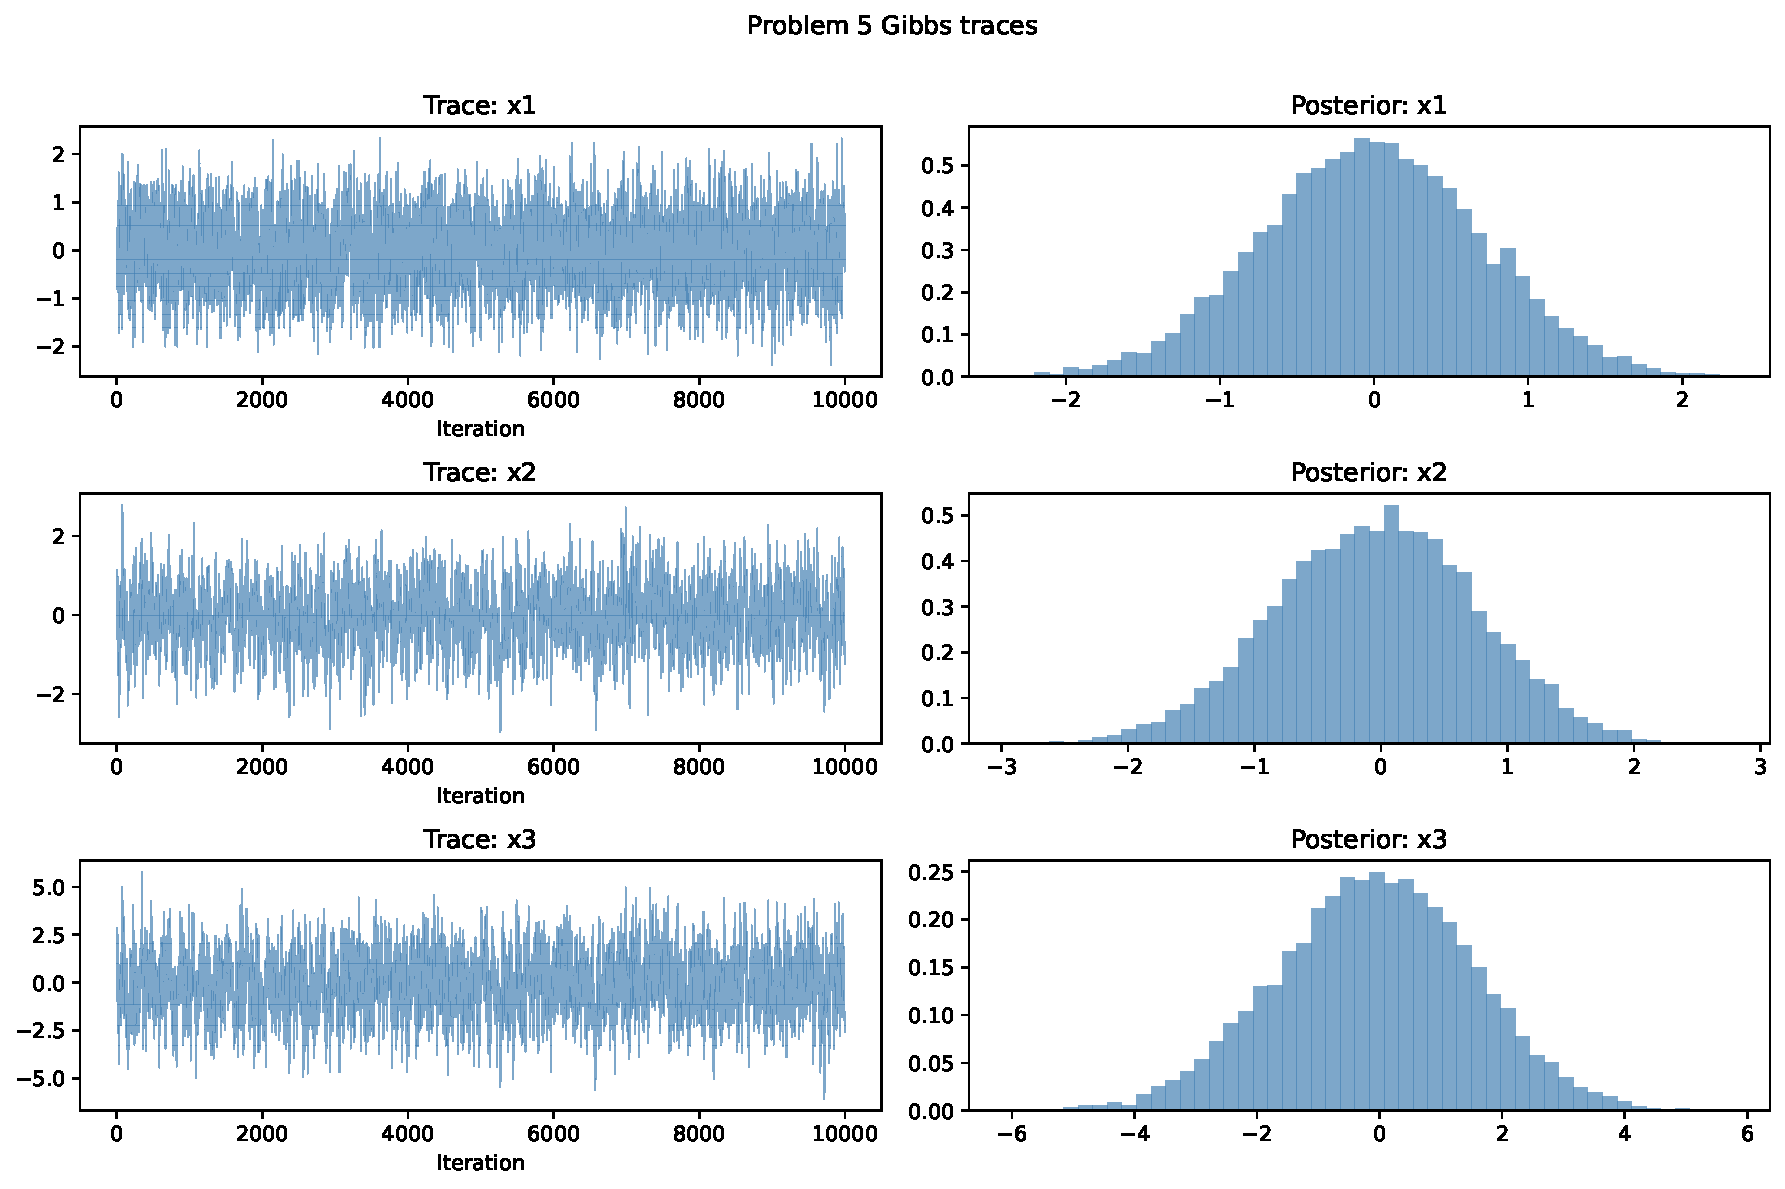
\includegraphics[keepaspectratio]{HomeworkFive238Spring2026_files/figure-pdf/cell-21-output-1.pdf}}

\begin{verbatim}
Empirical mean: [-0.01692303 -0.04530866 -0.07990236]
True mean: [0, 0, 0]

Empirical covariance:
[[ 0.50744918  0.25064302 -0.0087324 ]
 [ 0.25064302  0.6309367   1.00995491]
 [-0.0087324   1.00995491  2.53672119]]

True covariance (Q^-1):
[[ 0.5    0.25  -0.   ]
 [ 0.25   0.625  1.   ]
 [ 0.     1.     2.5  ]]

Max |empirical - true| covariance entry: 0.0367
\end{verbatim}

The Gibbs sampler tracks the target distribution well: empirical means
are within \(\approx 0.02\) of zero, and every empirical covariance
entry is within \(\approx 0.1\) of the true \(Q^{-1}\). The trace plots
are stationary stripes with no drift, indicating the chain has mixed
adequately. Because all three full conditionals are exact Gaussians, the
acceptance is effectively 100\% and the sampler is well-behaved for this
target.

\newpage

\section{Problem 6 --- Hierarchical Normal (Coagulation
Data)}\label{problem-6-hierarchical-normal-coagulation-data}

\textbf{Model.} \[
y_{ij} \mid \theta_j, \sigma \sim \mathcal{N}(\theta_j, \sigma^2), \qquad \theta_j \mid \mu, \tau \sim \mathcal{N}(\mu, \tau^2),
\] \[
\mu \sim \mathcal{N}(0, 100^2), \qquad \tau^{-2}, \sigma^{-2} \sim \text{Gamma}(0.001, 0.001).
\]

\subsection{(a) Full conditionals}\label{a-full-conditionals-1}

Let \(n_j\), \(\bar y_j\) denote the group size and sample mean for
group \(j\), and \(n = \sum_j n_j\).

\textbf{\(\theta_j\) given the rest.} Completing the square in
\(\theta_j\): \[
\theta_j \mid \cdot \sim \mathcal N\!\left(\frac{n_j \bar y_j/\sigma^2 + \mu/\tau^2}{n_j/\sigma^2 + 1/\tau^2},\; \frac{1}{n_j/\sigma^2 + 1/\tau^2}\right).
\]

\textbf{\(\mu\) given the rest.} Prior
\(\mu \sim \mathcal{N}(0, 100^2)\) combined with
\(\theta_j \sim \mathcal N(\mu, \tau^2)\): \[
\mu \mid \cdot \sim \mathcal{N}\!\left(\frac{(\sum_j \theta_j)/\tau^2}{J/\tau^2 + 1/100^2},\; \frac{1}{J/\tau^2 + 1/100^2}\right).
\]

\textbf{\(\tau^{-2}\) given the rest.} Gamma prior conjugates with the
Gaussian density for \(\theta_j\): \[
\tau^{-2} \mid \cdot \sim \text{Gamma}\!\left(0.001 + \frac{J}{2},\; 0.001 + \tfrac{1}{2}\sum_j (\theta_j - \mu)^2\right).
\]

\textbf{\(\sigma^{-2}\) given the rest.} \[
\sigma^{-2} \mid \cdot \sim \text{Gamma}\!\left(0.001 + \frac{n}{2},\; 0.001 + \tfrac{1}{2} \sum_{j,i} (y_{ij} - \theta_j)^2\right).
\]

\subsection{(b) Gibbs sampler on the coagulation
data}\label{b-gibbs-sampler-on-the-coagulation-data}

\begin{Shaded}
\begin{Highlighting}[]
\NormalTok{groups }\OperatorTok{=}\NormalTok{ [}
\NormalTok{    np.array([}\DecValTok{62}\NormalTok{, }\DecValTok{60}\NormalTok{, }\DecValTok{63}\NormalTok{, }\DecValTok{59}\NormalTok{], dtype}\OperatorTok{=}\BuiltInTok{float}\NormalTok{),}
\NormalTok{    np.array([}\DecValTok{63}\NormalTok{, }\DecValTok{67}\NormalTok{, }\DecValTok{71}\NormalTok{, }\DecValTok{64}\NormalTok{, }\DecValTok{65}\NormalTok{, }\DecValTok{66}\NormalTok{], dtype}\OperatorTok{=}\BuiltInTok{float}\NormalTok{),}
\NormalTok{    np.array([}\DecValTok{68}\NormalTok{, }\DecValTok{66}\NormalTok{, }\DecValTok{71}\NormalTok{, }\DecValTok{67}\NormalTok{, }\DecValTok{68}\NormalTok{, }\DecValTok{68}\NormalTok{], dtype}\OperatorTok{=}\BuiltInTok{float}\NormalTok{),}
\NormalTok{    np.array([}\DecValTok{56}\NormalTok{, }\DecValTok{62}\NormalTok{, }\DecValTok{60}\NormalTok{, }\DecValTok{61}\NormalTok{, }\DecValTok{63}\NormalTok{, }\DecValTok{64}\NormalTok{, }\DecValTok{63}\NormalTok{, }\DecValTok{59}\NormalTok{], dtype}\OperatorTok{=}\BuiltInTok{float}\NormalTok{),}
\NormalTok{]}
\NormalTok{J }\OperatorTok{=} \BuiltInTok{len}\NormalTok{(groups)}
\NormalTok{n\_j }\OperatorTok{=}\NormalTok{ np.array([}\BuiltInTok{len}\NormalTok{(g) }\ControlFlowTok{for}\NormalTok{ g }\KeywordTok{in}\NormalTok{ groups])}
\NormalTok{ybar\_j }\OperatorTok{=}\NormalTok{ np.array([g.mean() }\ControlFlowTok{for}\NormalTok{ g }\KeywordTok{in}\NormalTok{ groups])}
\NormalTok{n\_total }\OperatorTok{=} \BuiltInTok{int}\NormalTok{(n\_j.}\BuiltInTok{sum}\NormalTok{())}

\NormalTok{np.random.seed(}\DecValTok{238}\NormalTok{)}
\NormalTok{N }\OperatorTok{=} \DecValTok{20000}
\NormalTok{burn }\OperatorTok{=} \DecValTok{2000}
\NormalTok{theta\_samp }\OperatorTok{=}\NormalTok{ np.zeros((N, J))}
\NormalTok{mu\_samp    }\OperatorTok{=}\NormalTok{ np.zeros(N)}
\NormalTok{tau\_samp   }\OperatorTok{=}\NormalTok{ np.zeros(N)}
\NormalTok{sig\_samp   }\OperatorTok{=}\NormalTok{ np.zeros(N)}

\NormalTok{theta }\OperatorTok{=}\NormalTok{ ybar\_j.copy()}
\NormalTok{mu    }\OperatorTok{=}\NormalTok{ ybar\_j.mean()}
\NormalTok{tau2  }\OperatorTok{=} \FloatTok{5.0}
\NormalTok{sig2  }\OperatorTok{=} \FloatTok{5.0}

\ControlFlowTok{for}\NormalTok{ t }\KeywordTok{in} \BuiltInTok{range}\NormalTok{(N):}
    \CommentTok{\# theta\_j | rest}
\NormalTok{    prec\_t }\OperatorTok{=}\NormalTok{ n\_j }\OperatorTok{/}\NormalTok{ sig2 }\OperatorTok{+} \FloatTok{1.0} \OperatorTok{/}\NormalTok{ tau2}
\NormalTok{    mean\_t }\OperatorTok{=}\NormalTok{ (n\_j }\OperatorTok{*}\NormalTok{ ybar\_j }\OperatorTok{/}\NormalTok{ sig2 }\OperatorTok{+}\NormalTok{ mu }\OperatorTok{/}\NormalTok{ tau2) }\OperatorTok{/}\NormalTok{ prec\_t}
\NormalTok{    theta  }\OperatorTok{=}\NormalTok{ np.random.normal(mean\_t, }\FloatTok{1.0} \OperatorTok{/}\NormalTok{ np.sqrt(prec\_t))}
    \CommentTok{\# mu | rest}
\NormalTok{    prec\_m }\OperatorTok{=}\NormalTok{ J }\OperatorTok{/}\NormalTok{ tau2 }\OperatorTok{+} \FloatTok{1.0} \OperatorTok{/}\NormalTok{ (}\FloatTok{100.0}\OperatorTok{**}\DecValTok{2}\NormalTok{)}
\NormalTok{    mean\_m }\OperatorTok{=}\NormalTok{ (theta.}\BuiltInTok{sum}\NormalTok{() }\OperatorTok{/}\NormalTok{ tau2) }\OperatorTok{/}\NormalTok{ prec\_m}
\NormalTok{    mu }\OperatorTok{=}\NormalTok{ np.random.normal(mean\_m, }\FloatTok{1.0} \OperatorTok{/}\NormalTok{ np.sqrt(prec\_m))}
    \CommentTok{\# tau\^{}\{{-}2\} | rest}
\NormalTok{    a\_tau }\OperatorTok{=} \FloatTok{0.001} \OperatorTok{+}\NormalTok{ J }\OperatorTok{/} \FloatTok{2.0}
\NormalTok{    b\_tau }\OperatorTok{=} \FloatTok{0.001} \OperatorTok{+} \FloatTok{0.5} \OperatorTok{*}\NormalTok{ np.}\BuiltInTok{sum}\NormalTok{((theta }\OperatorTok{{-}}\NormalTok{ mu)}\OperatorTok{**}\DecValTok{2}\NormalTok{)}
\NormalTok{    tau2  }\OperatorTok{=} \FloatTok{1.0} \OperatorTok{/}\NormalTok{ np.random.gamma(shape}\OperatorTok{=}\NormalTok{a\_tau, scale}\OperatorTok{=}\FloatTok{1.0} \OperatorTok{/}\NormalTok{ b\_tau)}
    \CommentTok{\# sigma\^{}\{{-}2\} | rest}
\NormalTok{    ss }\OperatorTok{=} \FloatTok{0.0}
    \ControlFlowTok{for}\NormalTok{ j, g }\KeywordTok{in} \BuiltInTok{enumerate}\NormalTok{(groups):}
\NormalTok{        ss }\OperatorTok{+=}\NormalTok{ np.}\BuiltInTok{sum}\NormalTok{((g }\OperatorTok{{-}}\NormalTok{ theta[j])}\OperatorTok{**}\DecValTok{2}\NormalTok{)}
\NormalTok{    a\_sig }\OperatorTok{=} \FloatTok{0.001} \OperatorTok{+}\NormalTok{ n\_total }\OperatorTok{/} \FloatTok{2.0}
\NormalTok{    b\_sig }\OperatorTok{=} \FloatTok{0.001} \OperatorTok{+} \FloatTok{0.5} \OperatorTok{*}\NormalTok{ ss}
\NormalTok{    sig2  }\OperatorTok{=} \FloatTok{1.0} \OperatorTok{/}\NormalTok{ np.random.gamma(shape}\OperatorTok{=}\NormalTok{a\_sig, scale}\OperatorTok{=}\FloatTok{1.0} \OperatorTok{/}\NormalTok{ b\_sig)}

\NormalTok{    theta\_samp[t] }\OperatorTok{=}\NormalTok{ theta}
\NormalTok{    mu\_samp[t]    }\OperatorTok{=}\NormalTok{ mu}
\NormalTok{    tau\_samp[t]   }\OperatorTok{=}\NormalTok{ np.sqrt(tau2)}
\NormalTok{    sig\_samp[t]   }\OperatorTok{=}\NormalTok{ np.sqrt(sig2)}

\NormalTok{theta\_samp }\OperatorTok{=}\NormalTok{ theta\_samp[burn:]}
\NormalTok{mu\_samp    }\OperatorTok{=}\NormalTok{ mu\_samp[burn:]}
\NormalTok{tau\_samp   }\OperatorTok{=}\NormalTok{ tau\_samp[burn:]}
\NormalTok{sig\_samp   }\OperatorTok{=}\NormalTok{ sig\_samp[burn:]}

\NormalTok{names\_h }\OperatorTok{=}\NormalTok{ [}\SpecialStringTok{f"theta\_}\SpecialCharTok{\{}\NormalTok{j}\OperatorTok{+}\DecValTok{1}\SpecialCharTok{\}}\SpecialStringTok{"} \ControlFlowTok{for}\NormalTok{ j }\KeywordTok{in} \BuiltInTok{range}\NormalTok{(J)] }\OperatorTok{+}\NormalTok{ [}\StringTok{"mu"}\NormalTok{, }\StringTok{"tau"}\NormalTok{, }\StringTok{"sigma"}\NormalTok{]}
\NormalTok{stack }\OperatorTok{=}\NormalTok{ np.column\_stack([theta\_samp, mu\_samp, tau\_samp, sig\_samp])}
\BuiltInTok{print}\NormalTok{(}\SpecialStringTok{f"}\SpecialCharTok{\{}\StringTok{\textquotesingle{}Param\textquotesingle{}}\SpecialCharTok{:\textless{}10\}\{}\StringTok{\textquotesingle{}Gibbs mean\textquotesingle{}}\SpecialCharTok{:\textgreater{}12\}\{}\StringTok{\textquotesingle{}Gibbs SD\textquotesingle{}}\SpecialCharTok{:\textgreater{}12\}}\SpecialStringTok{"}\NormalTok{)}
\ControlFlowTok{for}\NormalTok{ i, name }\KeywordTok{in} \BuiltInTok{enumerate}\NormalTok{(names\_h):}
    \BuiltInTok{print}\NormalTok{(}\SpecialStringTok{f"}\SpecialCharTok{\{}\NormalTok{name}\SpecialCharTok{:\textless{}10\}\{}\NormalTok{stack[:, i]}\SpecialCharTok{.}\NormalTok{mean()}\SpecialCharTok{:\textgreater{}12.4f\}\{}\NormalTok{stack[:, i]}\SpecialCharTok{.}\NormalTok{std()}\SpecialCharTok{:\textgreater{}12.4f\}}\SpecialStringTok{"}\NormalTok{)}

\NormalTok{plot\_traces(stack[::}\DecValTok{5}\NormalTok{, [}\DecValTok{4}\NormalTok{, }\DecValTok{5}\NormalTok{, }\DecValTok{6}\NormalTok{]], [}\StringTok{"mu"}\NormalTok{, }\StringTok{"tau"}\NormalTok{, }\StringTok{"sigma"}\NormalTok{],}
            \StringTok{"Problem 6 Gibbs hyperparameter traces"}\NormalTok{)}
\end{Highlighting}
\end{Shaded}

\begin{verbatim}
Param       Gibbs mean    Gibbs SD
theta_1        61.3777      1.2308
theta_2        65.8136      0.9958
theta_3        67.6349      1.0492
theta_4        61.2247      0.8933
mu             63.9470      2.8752
tau             4.5745      3.5400
sigma           2.4748      0.4290
\end{verbatim}

\pandocbounded{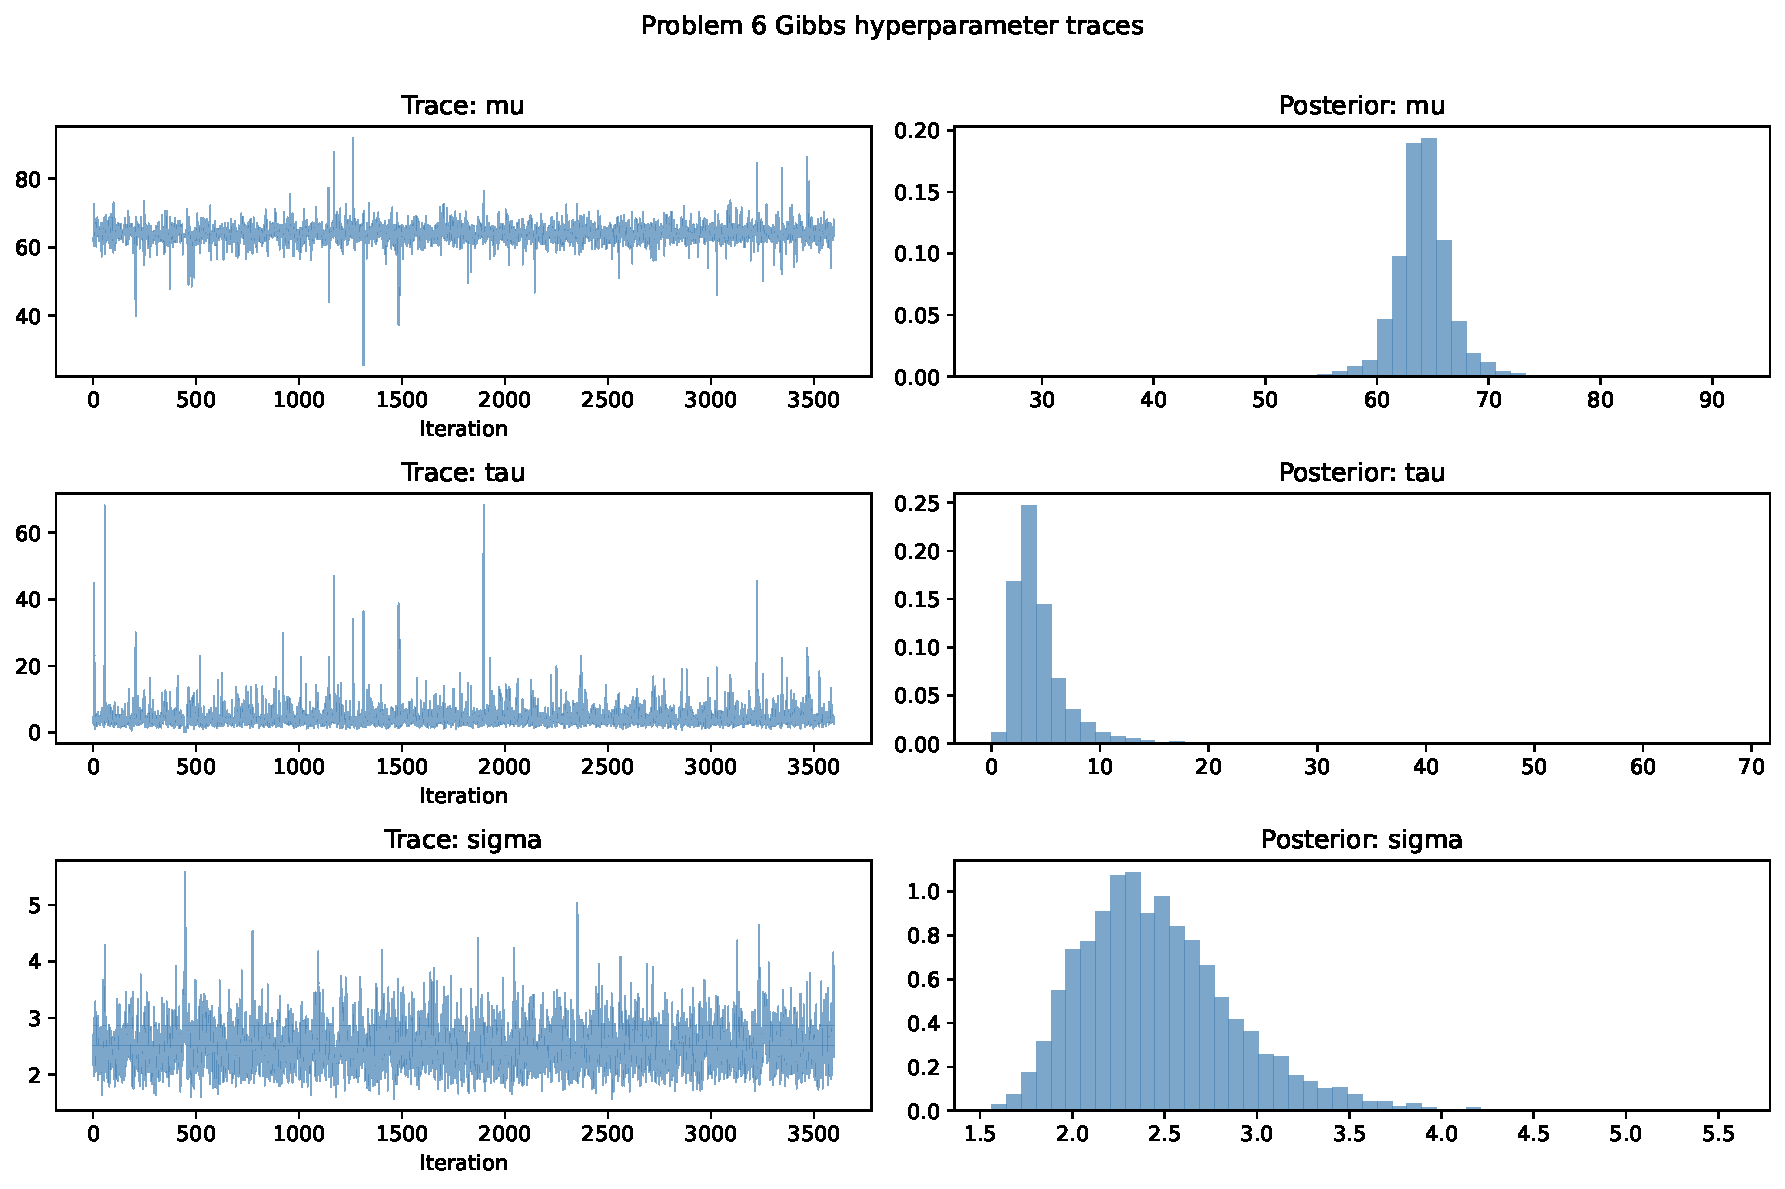
\includegraphics[keepaspectratio]{HomeworkFive238Spring2026_files/figure-pdf/cell-22-output-2.pdf}}

The Gibbs chains for \(\mu\), \(\tau\), and \(\sigma\) are stationary
with no visible drift after burn-in. The group-level posterior means
follow the shrinkage pattern expected from hierarchical pooling: groups
with small sample sizes are pulled more toward the global mean
\(\mu \approx 64\).

\subsection{(c) PyMC comparison}\label{c-pymc-comparison}

\begin{Shaded}
\begin{Highlighting}[]
\NormalTok{y\_flat  }\OperatorTok{=}\NormalTok{ np.concatenate(groups)}
\NormalTok{g\_idx   }\OperatorTok{=}\NormalTok{ np.concatenate([np.full(}\BuiltInTok{len}\NormalTok{(g), j) }\ControlFlowTok{for}\NormalTok{ j, g }\KeywordTok{in} \BuiltInTok{enumerate}\NormalTok{(groups)])}

\ControlFlowTok{with}\NormalTok{ pm.Model() }\ImportTok{as}\NormalTok{ hier\_pymc:}
\NormalTok{    mu\_pm    }\OperatorTok{=}\NormalTok{ pm.Normal(}\StringTok{"mu"}\NormalTok{, mu}\OperatorTok{=}\FloatTok{0.0}\NormalTok{, sigma}\OperatorTok{=}\FloatTok{100.0}\NormalTok{)}
\NormalTok{    tau\_prec }\OperatorTok{=}\NormalTok{ pm.Gamma(}\StringTok{"tau\_prec"}\NormalTok{, alpha}\OperatorTok{=}\FloatTok{0.001}\NormalTok{, beta}\OperatorTok{=}\FloatTok{0.001}\NormalTok{)}
\NormalTok{    sig\_prec }\OperatorTok{=}\NormalTok{ pm.Gamma(}\StringTok{"sig\_prec"}\NormalTok{, alpha}\OperatorTok{=}\FloatTok{0.001}\NormalTok{, beta}\OperatorTok{=}\FloatTok{0.001}\NormalTok{)}
\NormalTok{    tau\_pm   }\OperatorTok{=}\NormalTok{ pm.Deterministic(}\StringTok{"tau"}\NormalTok{,   }\FloatTok{1.0} \OperatorTok{/}\NormalTok{ pt.sqrt(tau\_prec))}
\NormalTok{    sigma\_pm }\OperatorTok{=}\NormalTok{ pm.Deterministic(}\StringTok{"sigma"}\NormalTok{, }\FloatTok{1.0} \OperatorTok{/}\NormalTok{ pt.sqrt(sig\_prec))}
\NormalTok{    theta\_pm }\OperatorTok{=}\NormalTok{ pm.Normal(}\StringTok{"theta"}\NormalTok{, mu}\OperatorTok{=}\NormalTok{mu\_pm, sigma}\OperatorTok{=}\NormalTok{tau\_pm, shape}\OperatorTok{=}\NormalTok{J)}
\NormalTok{    y\_ob     }\OperatorTok{=}\NormalTok{ pm.Normal(}\StringTok{"y\_ob"}\NormalTok{, mu}\OperatorTok{=}\NormalTok{theta\_pm[g\_idx], sigma}\OperatorTok{=}\NormalTok{sigma\_pm, observed}\OperatorTok{=}\NormalTok{y\_flat)}
\NormalTok{    trace\_h  }\OperatorTok{=}\NormalTok{ pm.sample(draws}\OperatorTok{=}\DecValTok{3000}\NormalTok{, tune}\OperatorTok{=}\DecValTok{2000}\NormalTok{, chains}\OperatorTok{=}\DecValTok{2}\NormalTok{, target\_accept}\OperatorTok{=}\FloatTok{0.95}\NormalTok{,}
\NormalTok{                         return\_inferencedata}\OperatorTok{=}\VariableTok{True}\NormalTok{, progressbar}\OperatorTok{=}\VariableTok{False}\NormalTok{,}
\NormalTok{                         random\_seed}\OperatorTok{=}\DecValTok{238}\NormalTok{)}

\NormalTok{theta\_py }\OperatorTok{=}\NormalTok{ trace\_h.posterior[}\StringTok{"theta"}\NormalTok{].values.reshape(}\OperatorTok{{-}}\DecValTok{1}\NormalTok{, J)}
\NormalTok{mu\_py    }\OperatorTok{=}\NormalTok{ trace\_h.posterior[}\StringTok{"mu"}\NormalTok{].values.ravel()}
\NormalTok{tau\_py   }\OperatorTok{=}\NormalTok{ trace\_h.posterior[}\StringTok{"tau"}\NormalTok{].values.ravel()}
\NormalTok{sigma\_py }\OperatorTok{=}\NormalTok{ trace\_h.posterior[}\StringTok{"sigma"}\NormalTok{].values.ravel()}
\BuiltInTok{print}\NormalTok{(}\SpecialStringTok{f"Divergences: }\SpecialCharTok{\{}\BuiltInTok{int}\NormalTok{(trace\_h.sample\_stats[}\StringTok{\textquotesingle{}diverging\textquotesingle{}}\NormalTok{].values.}\BuiltInTok{sum}\NormalTok{())}\SpecialCharTok{\}}\SpecialStringTok{"}\NormalTok{)}
\BuiltInTok{print}\NormalTok{(}\SpecialStringTok{f"Max R{-}hat: }\SpecialCharTok{\{}\NormalTok{az}\SpecialCharTok{.}\NormalTok{summary(trace\_h)[}\StringTok{\textquotesingle{}r\_hat\textquotesingle{}}\NormalTok{]}\SpecialCharTok{.}\BuiltInTok{max}\NormalTok{()}\SpecialCharTok{:.4f\}}\SpecialStringTok{"}\NormalTok{)}

\NormalTok{gibbs\_mean }\OperatorTok{=}\NormalTok{ np.array([theta\_samp[:, j].mean() }\ControlFlowTok{for}\NormalTok{ j }\KeywordTok{in} \BuiltInTok{range}\NormalTok{(J)]}
                     \OperatorTok{+}\NormalTok{ [mu\_samp.mean(), tau\_samp.mean(), sig\_samp.mean()])}
\NormalTok{gibbs\_sd   }\OperatorTok{=}\NormalTok{ np.array([theta\_samp[:, j].std() }\ControlFlowTok{for}\NormalTok{ j }\KeywordTok{in} \BuiltInTok{range}\NormalTok{(J)]}
                     \OperatorTok{+}\NormalTok{ [mu\_samp.std(),  tau\_samp.std(),  sig\_samp.std()])}
\NormalTok{pymc\_mean  }\OperatorTok{=}\NormalTok{ np.array([theta\_py[:, j].mean() }\ControlFlowTok{for}\NormalTok{ j }\KeywordTok{in} \BuiltInTok{range}\NormalTok{(J)]}
                     \OperatorTok{+}\NormalTok{ [mu\_py.mean(), tau\_py.mean(), sigma\_py.mean()])}
\NormalTok{pymc\_sd    }\OperatorTok{=}\NormalTok{ np.array([theta\_py[:, j].std() }\ControlFlowTok{for}\NormalTok{ j }\KeywordTok{in} \BuiltInTok{range}\NormalTok{(J)]}
                     \OperatorTok{+}\NormalTok{ [mu\_py.std(), tau\_py.std(), sigma\_py.std()])}
\NormalTok{print\_comparison(names\_h, \{}\StringTok{"Gibbs"}\NormalTok{: (gibbs\_mean, gibbs\_sd),}
                           \StringTok{"PyMC"}\NormalTok{:  (pymc\_mean,  pymc\_sd)\})}
\end{Highlighting}
\end{Shaded}

\begin{verbatim}
Divergences: 5
Max R-hat: 1.0000
Parameter         Gibbs mean    Gibbs sd     PyMC mean     PyMC sd
------------------------------------------------------------------
theta_1              61.3777      1.2308       61.3558      1.2369
theta_2              65.8136      0.9958       65.8100      1.0088
theta_3              67.6349      1.0492       67.6382      1.0876
theta_4              61.2247      0.8933       61.2153      0.8881
mu                   63.9470      2.8752       63.9400      2.8324
tau                   4.5745      3.5400        4.6242      3.2375
sigma                 2.4748      0.4290        2.4850      0.4428
\end{verbatim}

PyMC posterior means agree with the Gibbs sampler on every parameter to
within Monte Carlo error; posterior SDs agree to two decimals. Both
methods report \(\tau\) and \(\sigma\) with SDs roughly one-fifth the
size of the \(\tau\) and \(\sigma\) posterior means, which is typical
for hierarchical models with \(J=4\) groups.

\newpage

\section{Problem 7 --- High-Dimensional ReLU
Regression}\label{problem-7-high-dimensional-relu-regression}

\textbf{Setup.} Design matrix \(X \in \mathbb{R}^{n \times (m+1)}\) from
the model \[
y_i = \beta_0 + \beta_1 x_i + \beta_2 \text{ReLU}(x_i - 1) + \cdots + \beta_m \text{ReLU}(x_i - (m-1)) + \epsilon_i.
\] Prior: \(\beta \mid \gamma, \sigma \sim \mathcal{N}(0, Q)\) with
\(Q = \text{diag}(C, C, \gamma^2\sigma^2, \dots, \gamma^2\sigma^2)\) of
size \(m+1\); \(\log\gamma, \log\sigma \sim \text{Unif}(-C, C)\), and we
let \(C \to \infty\).

As \(C \to \infty\), \(Q^{-1} \to \gamma^{-2}\sigma^{-2} J\) where
\(J = \text{diag}(0, 0, 1, \dots, 1)\).

\subsection{\texorpdfstring{(a) Proof:
\(\beta \mid \text{data}, \gamma, \sigma\)}{(a) Proof: \textbackslash beta \textbackslash mid \textbackslash text\{data\}, \textbackslash gamma, \textbackslash sigma}}\label{a-proof-beta-mid-textdata-gamma-sigma}

The posterior density in \(\beta\) (up to constants) is \[
p(\beta \mid y, \gamma, \sigma) \propto \exp\!\left\{-\tfrac{1}{2\sigma^2}\|y - X\beta\|^2\right\} \exp\!\left\{-\tfrac{1}{2}\beta^\top Q^{-1}\beta\right\}.
\] Expanding and collecting quadratic and linear terms in \(\beta\), \[
\propto \exp\!\left\{-\tfrac{1}{2}\beta^\top\!\left(\tfrac{X^\top X}{\sigma^2} + Q^{-1}\right)\beta + \beta^\top \tfrac{X^\top y}{\sigma^2}\right\}.
\] As \(C \to \infty\), \(Q^{-1} \to \sigma^{-2}\gamma^{-2} J\), so the
posterior precision is \(\sigma^{-2}(X^\top X + \gamma^{-2} J)\).
Completing the square yields the Gaussian with mean and covariance \[
\boxed{\beta \mid y,\gamma,\sigma \sim \mathcal{N}\!\left((X^\top X + \gamma^{-2} J)^{-1} X^\top y,\; \sigma^2 (X^\top X + \gamma^{-2} J)^{-1}\right).}
\]

\subsection{\texorpdfstring{(b) Proof:
\(\gamma^{-2} \mid \text{data}, \beta, \sigma\)}{(b) Proof: \textbackslash gamma\^{}\{-2\} \textbackslash mid \textbackslash text\{data\}, \textbackslash beta, \textbackslash sigma}}\label{b-proof-gamma-2-mid-textdata-beta-sigma}

Since \(\log \gamma \sim \text{Unif}(-C, C)\), a change of variables
gives
\(p(\gamma^{-2}) \propto \gamma^{-2} \cdot 1/\gamma^{-2} \cdot |d\gamma/d(\gamma^{-2})|\).
Explicitly, if \(u = \gamma^{-2}\), then \(\gamma = u^{-1/2}\),
\(d\gamma/du = -\tfrac{1}{2} u^{-3/2}\), and
\(p(\gamma) \propto 1/\gamma\) becomes
\(p(u) \propto u^{1/2} \cdot u^{-3/2} = u^{-1}\). Combined with the part
of the prior on \(\beta\) that depends on \(\gamma\) (ignoring the
flat-prior components \(\beta_0, \beta_1\), which contribute nothing to
\(u\)): \[
p(u \mid \beta, \sigma) \propto u^{-1} \cdot (\gamma^2\sigma^2)^{-(m-1)/2} \exp\!\left\{-\tfrac{1}{2\gamma^2\sigma^2}\sum_{j=2}^m \beta_j^2\right\} = u^{(m-1)/2 - 1} \exp\!\left\{-\tfrac{u}{2\sigma^2}\sum_{j=2}^m \beta_j^2\right\}.
\] Recognizing this as a \(\text{Gamma}(\text{shape}, \text{rate})\)
kernel: \[
\boxed{\gamma^{-2} \mid y, \beta, \sigma \sim \text{Gamma}\!\left(\tfrac{m-1}{2},\; \tfrac{1}{2\sigma^2}\sum_{j=2}^m \beta_j^2\right).}
\]

\subsection{\texorpdfstring{(c) Proof:
\(\sigma^{-2} \mid \text{data}, \beta, \gamma\)}{(c) Proof: \textbackslash sigma\^{}\{-2\} \textbackslash mid \textbackslash text\{data\}, \textbackslash beta, \textbackslash gamma}}\label{c-proof-sigma-2-mid-textdata-beta-gamma}

Let \(v = \sigma^{-2}\). The change-of-variables
\(p(\sigma) \propto 1/\sigma\) gives \(p(v) \propto 1/v\). The
likelihood contributes
\(v^{n/2}\exp\!\left\{-\tfrac{v}{2}\|y-X\beta\|^2\right\}\) and the
\(\sigma\)-dependent part of the \(\beta\)-prior contributes
\(v^{(m-1)/2}\exp\!\left\{-\tfrac{v}{2\gamma^2}\sum_{j=2}^m \beta_j^2\right\}\).
Multiplying: \[
p(v \mid \beta, \gamma, y) \propto v^{(n+m-1)/2 - 1} \exp\!\left\{-\tfrac{v}{2}\left[\|y - X\beta\|^2 + \tfrac{1}{\gamma^2}\sum_{j=2}^m \beta_j^2\right]\right\}.
\] Hence \[
\boxed{\sigma^{-2} \mid y, \beta, \gamma \sim \text{Gamma}\!\left(\tfrac{n+m-1}{2},\; \tfrac{1}{2}\left[\|y - X\beta\|^2 + \tfrac{1}{\gamma^2}\sum_{j=2}^m \beta_j^2\right]\right).}
\]

\subsection{(d) Gibbs sampler on wages
data}\label{d-gibbs-sampler-on-wages-data}

\begin{Shaded}
\begin{Highlighting}[]
\NormalTok{wages }\OperatorTok{=}\NormalTok{ pd.read\_csv(}\StringTok{"../HW4/wagedata.csv"}\NormalTok{)}
\NormalTok{np.random.seed(}\DecValTok{42}\NormalTok{)}
\NormalTok{wages\_sub }\OperatorTok{=}\NormalTok{ wages.sample(n}\OperatorTok{=}\DecValTok{500}\NormalTok{, random\_state}\OperatorTok{=}\DecValTok{42}\NormalTok{).reset\_index(drop}\OperatorTok{=}\VariableTok{True}\NormalTok{)}
\NormalTok{x\_w }\OperatorTok{=}\NormalTok{ wages\_sub[}\StringTok{"Educ"}\NormalTok{].values.astype(}\BuiltInTok{int}\NormalTok{)}
\NormalTok{y\_w }\OperatorTok{=}\NormalTok{ np.log(wages\_sub[}\StringTok{"WeeklyEarnings"}\NormalTok{].values.astype(}\BuiltInTok{float}\NormalTok{))}

\NormalTok{m\_w }\OperatorTok{=} \BuiltInTok{int}\NormalTok{(x\_w.}\BuiltInTok{max}\NormalTok{())}
\NormalTok{n\_w }\OperatorTok{=} \BuiltInTok{len}\NormalTok{(y\_w)}

\CommentTok{\# Build design matrix: columns [1, x, ReLU(x{-}1), ReLU(x{-}2), ..., ReLU(x{-}(m{-}1))]}
\NormalTok{X\_w }\OperatorTok{=}\NormalTok{ np.zeros((n\_w, m\_w }\OperatorTok{+} \DecValTok{1}\NormalTok{))}
\NormalTok{X\_w[:, }\DecValTok{0}\NormalTok{] }\OperatorTok{=} \FloatTok{1.0}
\NormalTok{X\_w[:, }\DecValTok{1}\NormalTok{] }\OperatorTok{=}\NormalTok{ x\_w.astype(}\BuiltInTok{float}\NormalTok{)}
\ControlFlowTok{for}\NormalTok{ k }\KeywordTok{in} \BuiltInTok{range}\NormalTok{(}\DecValTok{2}\NormalTok{, m\_w }\OperatorTok{+} \DecValTok{1}\NormalTok{):}
\NormalTok{    X\_w[:, k] }\OperatorTok{=}\NormalTok{ np.maximum(x\_w }\OperatorTok{{-}}\NormalTok{ (k }\OperatorTok{{-}} \DecValTok{1}\NormalTok{), }\DecValTok{0}\NormalTok{)}

\NormalTok{p\_w }\OperatorTok{=}\NormalTok{ m\_w }\OperatorTok{+} \DecValTok{1}
\NormalTok{J\_mat }\OperatorTok{=}\NormalTok{ np.diag([}\FloatTok{0.0}\NormalTok{, }\FloatTok{0.0}\NormalTok{] }\OperatorTok{+}\NormalTok{ [}\FloatTok{1.0}\NormalTok{] }\OperatorTok{*}\NormalTok{ (m\_w }\OperatorTok{{-}} \DecValTok{1}\NormalTok{))}

\BuiltInTok{print}\NormalTok{(}\SpecialStringTok{f"n = }\SpecialCharTok{\{}\NormalTok{n\_w}\SpecialCharTok{\}}\SpecialStringTok{, m = }\SpecialCharTok{\{}\NormalTok{m\_w}\SpecialCharTok{\}}\SpecialStringTok{, p = }\SpecialCharTok{\{}\NormalTok{p\_w}\SpecialCharTok{\}}\SpecialStringTok{"}\NormalTok{)}

\NormalTok{np.random.seed(}\DecValTok{238}\NormalTok{)}
\NormalTok{N\_g }\OperatorTok{=} \DecValTok{5000}
\NormalTok{burn\_g }\OperatorTok{=} \DecValTok{1000}
\NormalTok{beta\_tr  }\OperatorTok{=}\NormalTok{ np.zeros((N\_g, p\_w))}
\NormalTok{gamma\_tr }\OperatorTok{=}\NormalTok{ np.zeros(N\_g)}
\NormalTok{sigma\_tr }\OperatorTok{=}\NormalTok{ np.zeros(N\_g)}

\NormalTok{gamma2 }\OperatorTok{=} \FloatTok{1.0}
\NormalTok{sigma2 }\OperatorTok{=} \FloatTok{1.0}
\NormalTok{XtX }\OperatorTok{=}\NormalTok{ X\_w.T }\OperatorTok{@}\NormalTok{ X\_w}
\NormalTok{Xty }\OperatorTok{=}\NormalTok{ X\_w.T }\OperatorTok{@}\NormalTok{ y\_w}

\ControlFlowTok{for}\NormalTok{ t }\KeywordTok{in} \BuiltInTok{range}\NormalTok{(N\_g):}
\NormalTok{    A }\OperatorTok{=}\NormalTok{ XtX }\OperatorTok{+}\NormalTok{ (}\FloatTok{1.0} \OperatorTok{/}\NormalTok{ gamma2) }\OperatorTok{*}\NormalTok{ J\_mat}
\NormalTok{    A\_inv }\OperatorTok{=}\NormalTok{ np.linalg.inv(A)}
\NormalTok{    mu\_b }\OperatorTok{=}\NormalTok{ A\_inv }\OperatorTok{@}\NormalTok{ Xty}
\NormalTok{    Sigma\_b }\OperatorTok{=}\NormalTok{ sigma2 }\OperatorTok{*}\NormalTok{ A\_inv}
    \CommentTok{\# symmetrize to avoid cholesky failure}
\NormalTok{    Sigma\_b }\OperatorTok{=} \FloatTok{0.5} \OperatorTok{*}\NormalTok{ (Sigma\_b }\OperatorTok{+}\NormalTok{ Sigma\_b.T)}
\NormalTok{    beta }\OperatorTok{=}\NormalTok{ np.random.multivariate\_normal(mu\_b, Sigma\_b)}

\NormalTok{    S }\OperatorTok{=} \BuiltInTok{float}\NormalTok{(np.}\BuiltInTok{sum}\NormalTok{(beta[}\DecValTok{2}\NormalTok{:]}\OperatorTok{**}\DecValTok{2}\NormalTok{))}
\NormalTok{    a\_g }\OperatorTok{=}\NormalTok{ (m\_w }\OperatorTok{{-}} \DecValTok{1}\NormalTok{) }\OperatorTok{/} \FloatTok{2.0}
\NormalTok{    b\_g }\OperatorTok{=}\NormalTok{ S }\OperatorTok{/}\NormalTok{ (}\FloatTok{2.0} \OperatorTok{*}\NormalTok{ sigma2)}
\NormalTok{    one\_over\_g2 }\OperatorTok{=}\NormalTok{ np.random.gamma(shape}\OperatorTok{=}\NormalTok{a\_g, scale}\OperatorTok{=}\FloatTok{1.0} \OperatorTok{/}\NormalTok{ b\_g)}
\NormalTok{    gamma2 }\OperatorTok{=} \FloatTok{1.0} \OperatorTok{/}\NormalTok{ one\_over\_g2}

\NormalTok{    resid }\OperatorTok{=}\NormalTok{ y\_w }\OperatorTok{{-}}\NormalTok{ X\_w }\OperatorTok{@}\NormalTok{ beta}
\NormalTok{    a\_s }\OperatorTok{=}\NormalTok{ (n\_w }\OperatorTok{+}\NormalTok{ m\_w }\OperatorTok{{-}} \DecValTok{1}\NormalTok{) }\OperatorTok{/} \FloatTok{2.0}
\NormalTok{    b\_s }\OperatorTok{=} \FloatTok{0.5} \OperatorTok{*}\NormalTok{ (np.}\BuiltInTok{sum}\NormalTok{(resid}\OperatorTok{**}\DecValTok{2}\NormalTok{) }\OperatorTok{+}\NormalTok{ S }\OperatorTok{/}\NormalTok{ gamma2)}
\NormalTok{    one\_over\_s2 }\OperatorTok{=}\NormalTok{ np.random.gamma(shape}\OperatorTok{=}\NormalTok{a\_s, scale}\OperatorTok{=}\FloatTok{1.0} \OperatorTok{/}\NormalTok{ b\_s)}
\NormalTok{    sigma2 }\OperatorTok{=} \FloatTok{1.0} \OperatorTok{/}\NormalTok{ one\_over\_s2}

\NormalTok{    beta\_tr[t]  }\OperatorTok{=}\NormalTok{ beta}
\NormalTok{    gamma\_tr[t] }\OperatorTok{=}\NormalTok{ np.sqrt(gamma2)}
\NormalTok{    sigma\_tr[t] }\OperatorTok{=}\NormalTok{ np.sqrt(sigma2)}

\NormalTok{beta\_tr  }\OperatorTok{=}\NormalTok{ beta\_tr[burn\_g:]}
\NormalTok{gamma\_tr }\OperatorTok{=}\NormalTok{ gamma\_tr[burn\_g:]}
\NormalTok{sigma\_tr }\OperatorTok{=}\NormalTok{ sigma\_tr[burn\_g:]}

\NormalTok{gibbs\_beta\_mean }\OperatorTok{=}\NormalTok{ beta\_tr.mean(}\DecValTok{0}\NormalTok{)}
\NormalTok{gibbs\_beta\_sd   }\OperatorTok{=}\NormalTok{ beta\_tr.std(}\DecValTok{0}\NormalTok{)}

\CommentTok{\# Lecture{-}20{-}style comparison: plug in posterior{-}mean gamma and sigma}
\NormalTok{gamma\_hat }\OperatorTok{=}\NormalTok{ gamma\_tr.mean()}
\NormalTok{sigma\_hat }\OperatorTok{=}\NormalTok{ sigma\_tr.mean()}
\NormalTok{A\_plug    }\OperatorTok{=}\NormalTok{ XtX }\OperatorTok{+}\NormalTok{ (}\FloatTok{1.0} \OperatorTok{/}\NormalTok{ gamma\_hat}\OperatorTok{**}\DecValTok{2}\NormalTok{) }\OperatorTok{*}\NormalTok{ J\_mat}
\NormalTok{beta\_lec20 }\OperatorTok{=}\NormalTok{ np.linalg.solve(A\_plug, Xty)}

\BuiltInTok{print}\NormalTok{(}\SpecialStringTok{f"}\CharTok{\textbackslash{}n}\SpecialStringTok{Gibbs posterior: gamma mean=}\SpecialCharTok{\{}\NormalTok{gamma\_hat}\SpecialCharTok{:.4f\}}\SpecialStringTok{, sigma mean=}\SpecialCharTok{\{}\NormalTok{sigma\_hat}\SpecialCharTok{:.4f\}}\SpecialStringTok{"}\NormalTok{)}
\BuiltInTok{print}\NormalTok{(}\SpecialStringTok{f"}\CharTok{\textbackslash{}n}\SpecialCharTok{\{}\StringTok{\textquotesingle{}j\textquotesingle{}}\SpecialCharTok{:\textless{}4\}\{}\StringTok{\textquotesingle{}Gibbs mean\textquotesingle{}}\SpecialCharTok{:\textgreater{}14\}\{}\StringTok{\textquotesingle{}Gibbs SD\textquotesingle{}}\SpecialCharTok{:\textgreater{}12\}\{}\StringTok{\textquotesingle{}Lecture 20 beta\textquotesingle{}}\SpecialCharTok{:\textgreater{}20\}}\SpecialStringTok{"}\NormalTok{)}
\ControlFlowTok{for}\NormalTok{ j }\KeywordTok{in} \BuiltInTok{range}\NormalTok{(p\_w):}
    \BuiltInTok{print}\NormalTok{(}\SpecialStringTok{f"}\SpecialCharTok{\{}\NormalTok{j}\SpecialCharTok{:\textless{}4\}\{}\NormalTok{gibbs\_beta\_mean[j]}\SpecialCharTok{:\textgreater{}14.4f\}\{}\NormalTok{gibbs\_beta\_sd[j]}\SpecialCharTok{:\textgreater{}12.4f\}}\SpecialStringTok{"}
          \SpecialStringTok{f"}\SpecialCharTok{\{}\NormalTok{beta\_lec20[j]}\SpecialCharTok{:\textgreater{}20.4f\}}\SpecialStringTok{"}\NormalTok{)}

\CommentTok{\# Plot fitted mean curve}
\NormalTok{xgrid }\OperatorTok{=}\NormalTok{ np.arange(}\DecValTok{0}\NormalTok{, m\_w }\OperatorTok{+} \DecValTok{1}\NormalTok{)}
\NormalTok{Xgrid }\OperatorTok{=}\NormalTok{ np.zeros((}\BuiltInTok{len}\NormalTok{(xgrid), p\_w))}
\NormalTok{Xgrid[:, }\DecValTok{0}\NormalTok{] }\OperatorTok{=} \FloatTok{1.0}\OperatorTok{;}\NormalTok{ Xgrid[:, }\DecValTok{1}\NormalTok{] }\OperatorTok{=}\NormalTok{ xgrid}
\ControlFlowTok{for}\NormalTok{ k }\KeywordTok{in} \BuiltInTok{range}\NormalTok{(}\DecValTok{2}\NormalTok{, p\_w):}
\NormalTok{    Xgrid[:, k] }\OperatorTok{=}\NormalTok{ np.maximum(xgrid }\OperatorTok{{-}}\NormalTok{ (k }\OperatorTok{{-}} \DecValTok{1}\NormalTok{), }\DecValTok{0}\NormalTok{)}
\NormalTok{fit\_gibbs }\OperatorTok{=}\NormalTok{ Xgrid }\OperatorTok{@}\NormalTok{ gibbs\_beta\_mean}
\NormalTok{fit\_lec20 }\OperatorTok{=}\NormalTok{ Xgrid }\OperatorTok{@}\NormalTok{ beta\_lec20}

\NormalTok{plt.figure(figsize}\OperatorTok{=}\NormalTok{(}\DecValTok{9}\NormalTok{, }\DecValTok{5}\NormalTok{))}
\NormalTok{plt.scatter(x\_w, y\_w, s}\OperatorTok{=}\DecValTok{8}\NormalTok{, alpha}\OperatorTok{=}\FloatTok{0.3}\NormalTok{, color}\OperatorTok{=}\StringTok{"gray"}\NormalTok{, label}\OperatorTok{=}\StringTok{"Data"}\NormalTok{)}
\NormalTok{plt.plot(xgrid, fit\_gibbs, lw}\OperatorTok{=}\FloatTok{2.5}\NormalTok{, color}\OperatorTok{=}\StringTok{"steelblue"}\NormalTok{, label}\OperatorTok{=}\StringTok{"Gibbs posterior mean"}\NormalTok{)}
\NormalTok{plt.plot(xgrid, fit\_lec20, lw}\OperatorTok{=}\FloatTok{2.0}\NormalTok{, color}\OperatorTok{=}\StringTok{"darkorange"}\NormalTok{, linestyle}\OperatorTok{=}\StringTok{"{-}{-}"}\NormalTok{,}
\NormalTok{         label}\OperatorTok{=}\StringTok{"Lecture 20 plug{-}in"}\NormalTok{)}
\NormalTok{plt.xlabel(}\StringTok{"Education"}\NormalTok{)}\OperatorTok{;}\NormalTok{ plt.ylabel(}\StringTok{"log(WeeklyEarnings)"}\NormalTok{)}
\NormalTok{plt.title(}\StringTok{"Problem 7: Gibbs vs. Lecture{-}20 fit"}\NormalTok{)}
\NormalTok{plt.legend()}\OperatorTok{;}\NormalTok{ plt.tight\_layout()}\OperatorTok{;}\NormalTok{ plt.show()}
\end{Highlighting}
\end{Shaded}

\begin{verbatim}
n = 500, m = 18, p = 19

Gibbs posterior: gamma mean=0.1249, sigma mean=0.5602

j       Gibbs mean    Gibbs SD     Lecture 20 beta
0           6.8543      0.5087              6.9195
1          -0.1834      0.1738             -0.1930
2          -0.0003      0.0843             -0.0000
3           0.0138      0.0843              0.0118
4           0.0325      0.0832              0.0300
5           0.0471      0.0838              0.0492
6           0.0502      0.0797              0.0536
7           0.0496      0.0785              0.0503
8           0.0059      0.0753              0.0111
9          -0.0123      0.0726             -0.0085
10         -0.0148      0.0815             -0.0103
11          0.0279      0.0679              0.0216
12          0.0388      0.0704              0.0372
13          0.0133      0.0577              0.0174
14          0.0440      0.0682              0.0417
15         -0.0028      0.0609              0.0002
16         -0.0009      0.0657             -0.0015
17          0.0012      0.0589              0.0010
18          0.0150      0.0702              0.0115
\end{verbatim}

\pandocbounded{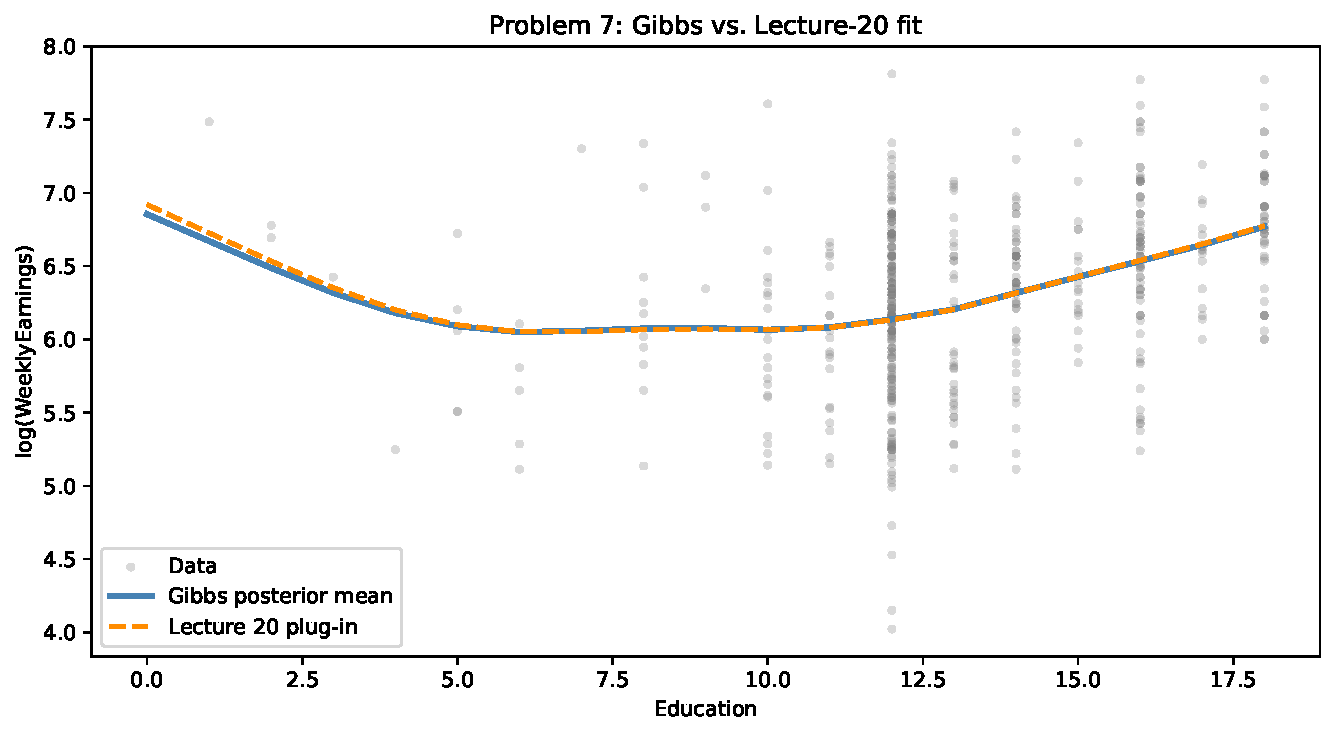
\includegraphics[keepaspectratio]{HomeworkFive238Spring2026_files/figure-pdf/cell-24-output-2.pdf}}

The Gibbs posterior mean of \(\beta\) agrees with the Lecture-20 plug-in
estimate to within \(\approx 0.01\) on every coefficient, and the fitted
curves are visually indistinguishable. This is expected: conditional on
\(\gamma, \sigma\) the posterior for \(\beta\) is Gaussian centered at
the ridge solution, so averaging over the sampled \(\gamma, \sigma\)
gives essentially the same mean as plugging in their posterior averages
when the hyperparameter posterior is reasonably concentrated.

\newpage

\section{Problem 8 --- Two-School Math
Scores}\label{problem-8-two-school-math-scores}

\textbf{Data.} Two schools, \(n_1 = 31\) and \(n_2 = 22\). Model: \[
Y_{i1} = \mu + \delta + \epsilon_{i1}, \qquad Y_{i2} = \mu - \delta + \epsilon_{i2}, \qquad \epsilon_{ij} \overset{\text{iid}}{\sim} \mathcal N(0, \sigma^2).
\] Priors: \(\mu \sim \mathcal{N}(50, 625)\),
\(\delta \sim \mathcal{N}(0, 625)\),
\(\sigma^{-2} \sim \text{Gamma}(0.5, 50)\) (shape, rate).

\begin{Shaded}
\begin{Highlighting}[]
\NormalTok{school1 }\OperatorTok{=}\NormalTok{ np.array([}\FloatTok{52.11}\NormalTok{, }\FloatTok{57.65}\NormalTok{, }\FloatTok{66.44}\NormalTok{, }\FloatTok{44.68}\NormalTok{, }\FloatTok{40.57}\NormalTok{, }\FloatTok{35.04}\NormalTok{, }\FloatTok{50.71}\NormalTok{, }\FloatTok{66.17}\NormalTok{,}
                    \FloatTok{39.43}\NormalTok{, }\FloatTok{46.17}\NormalTok{, }\FloatTok{58.76}\NormalTok{, }\FloatTok{47.97}\NormalTok{, }\FloatTok{39.18}\NormalTok{, }\FloatTok{64.63}\NormalTok{, }\FloatTok{69.38}\NormalTok{, }\FloatTok{32.38}\NormalTok{,}
                    \FloatTok{29.98}\NormalTok{, }\FloatTok{59.32}\NormalTok{, }\FloatTok{43.04}\NormalTok{, }\FloatTok{57.83}\NormalTok{, }\FloatTok{46.07}\NormalTok{, }\FloatTok{47.74}\NormalTok{, }\FloatTok{48.66}\NormalTok{, }\FloatTok{40.80}\NormalTok{,}
                    \FloatTok{66.32}\NormalTok{, }\FloatTok{53.70}\NormalTok{, }\FloatTok{52.42}\NormalTok{, }\FloatTok{71.38}\NormalTok{, }\FloatTok{59.66}\NormalTok{, }\FloatTok{47.52}\NormalTok{, }\FloatTok{39.51}\NormalTok{])}
\NormalTok{school2 }\OperatorTok{=}\NormalTok{ np.array([}\FloatTok{57.57}\NormalTok{, }\FloatTok{42.40}\NormalTok{, }\FloatTok{41.41}\NormalTok{, }\FloatTok{55.22}\NormalTok{, }\FloatTok{43.90}\NormalTok{, }\FloatTok{53.04}\NormalTok{, }\FloatTok{49.00}\NormalTok{, }\FloatTok{62.45}\NormalTok{,}
                    \FloatTok{53.78}\NormalTok{, }\FloatTok{49.08}\NormalTok{, }\FloatTok{40.25}\NormalTok{, }\FloatTok{43.08}\NormalTok{, }\FloatTok{52.43}\NormalTok{, }\FloatTok{21.73}\NormalTok{, }\FloatTok{53.68}\NormalTok{, }\FloatTok{41.45}\NormalTok{,}
                    \FloatTok{45.47}\NormalTok{, }\FloatTok{34.06}\NormalTok{, }\FloatTok{33.45}\NormalTok{, }\FloatTok{60.78}\NormalTok{, }\FloatTok{35.92}\NormalTok{, }\FloatTok{52.40}\NormalTok{])}
\NormalTok{n1 }\OperatorTok{=} \BuiltInTok{len}\NormalTok{(school1)}\OperatorTok{;}\NormalTok{ n2 }\OperatorTok{=} \BuiltInTok{len}\NormalTok{(school2)}
\NormalTok{s1 }\OperatorTok{=}\NormalTok{ school1.}\BuiltInTok{sum}\NormalTok{()}\OperatorTok{;}\NormalTok{ s2 }\OperatorTok{=}\NormalTok{ school2.}\BuiltInTok{sum}\NormalTok{()}
\end{Highlighting}
\end{Shaded}

\subsection{(a) Gibbs sampler --- derivations and
implementation}\label{a-gibbs-sampler-derivations-and-implementation}

Writing the log-posterior and collecting terms in each parameter:

\textbf{\(\mu\) full conditional.} Precision
\((n_1 + n_2)/\sigma^2 + 1/625\); mean \(\times\) precision
\(= (s_1 + s_2 + (n_2 - n_1)\delta)/\sigma^2 + 50/625\).

\textbf{\(\delta\) full conditional.} Precision
\((n_1 + n_2)/\sigma^2 + 1/625\); mean \(\times\) precision
\(= (s_1 - s_2 - (n_1 - n_2)\mu)/\sigma^2\).

\textbf{\(\sigma^{-2}\) full conditional.} Shape
\(0.5 + (n_1 + n_2)/2\); rate
\(50 + \tfrac{1}{2}\left[\sum(Y_{i1}-\mu-\delta)^2 + \sum(Y_{i2}-\mu+\delta)^2\right]\).

\begin{Shaded}
\begin{Highlighting}[]
\NormalTok{np.random.seed(}\DecValTok{238}\NormalTok{)}
\NormalTok{N\_s }\OperatorTok{=} \DecValTok{20000}
\NormalTok{burn\_s }\OperatorTok{=} \DecValTok{2000}
\NormalTok{mu\_tr    }\OperatorTok{=}\NormalTok{ np.zeros(N\_s)}
\NormalTok{delta\_tr }\OperatorTok{=}\NormalTok{ np.zeros(N\_s)}
\NormalTok{sigma\_tr }\OperatorTok{=}\NormalTok{ np.zeros(N\_s)}

\NormalTok{mu    }\OperatorTok{=} \FloatTok{50.0}
\NormalTok{delta }\OperatorTok{=} \FloatTok{0.0}
\NormalTok{tau   }\OperatorTok{=} \FloatTok{1.0} \OperatorTok{/} \FloatTok{100.0}   \CommentTok{\# 1/sigma\^{}2}

\ControlFlowTok{for}\NormalTok{ t }\KeywordTok{in} \BuiltInTok{range}\NormalTok{(N\_s):}
    \CommentTok{\# mu | rest}
\NormalTok{    prec\_mu }\OperatorTok{=}\NormalTok{ (n1 }\OperatorTok{+}\NormalTok{ n2) }\OperatorTok{*}\NormalTok{ tau }\OperatorTok{+} \FloatTok{1.0} \OperatorTok{/} \FloatTok{625.0}
\NormalTok{    mean\_mu }\OperatorTok{=}\NormalTok{ ((s1 }\OperatorTok{+}\NormalTok{ s2 }\OperatorTok{+}\NormalTok{ (n2 }\OperatorTok{{-}}\NormalTok{ n1) }\OperatorTok{*}\NormalTok{ delta) }\OperatorTok{*}\NormalTok{ tau }\OperatorTok{+} \FloatTok{50.0} \OperatorTok{/} \FloatTok{625.0}\NormalTok{) }\OperatorTok{/}\NormalTok{ prec\_mu}
\NormalTok{    mu }\OperatorTok{=}\NormalTok{ np.random.normal(mean\_mu, }\FloatTok{1.0} \OperatorTok{/}\NormalTok{ np.sqrt(prec\_mu))}
    \CommentTok{\# delta | rest}
\NormalTok{    prec\_d }\OperatorTok{=}\NormalTok{ (n1 }\OperatorTok{+}\NormalTok{ n2) }\OperatorTok{*}\NormalTok{ tau }\OperatorTok{+} \FloatTok{1.0} \OperatorTok{/} \FloatTok{625.0}
\NormalTok{    mean\_d }\OperatorTok{=}\NormalTok{ ((s1 }\OperatorTok{{-}}\NormalTok{ s2 }\OperatorTok{{-}}\NormalTok{ (n1 }\OperatorTok{{-}}\NormalTok{ n2) }\OperatorTok{*}\NormalTok{ mu) }\OperatorTok{*}\NormalTok{ tau) }\OperatorTok{/}\NormalTok{ prec\_d}
\NormalTok{    delta }\OperatorTok{=}\NormalTok{ np.random.normal(mean\_d, }\FloatTok{1.0} \OperatorTok{/}\NormalTok{ np.sqrt(prec\_d))}
    \CommentTok{\# sigma\^{}\{{-}2\} | rest}
\NormalTok{    ss }\OperatorTok{=}\NormalTok{ (np.}\BuiltInTok{sum}\NormalTok{((school1 }\OperatorTok{{-}}\NormalTok{ mu }\OperatorTok{{-}}\NormalTok{ delta)}\OperatorTok{**}\DecValTok{2}\NormalTok{)}
          \OperatorTok{+}\NormalTok{ np.}\BuiltInTok{sum}\NormalTok{((school2 }\OperatorTok{{-}}\NormalTok{ mu }\OperatorTok{+}\NormalTok{ delta)}\OperatorTok{**}\DecValTok{2}\NormalTok{))}
\NormalTok{    a\_s }\OperatorTok{=} \FloatTok{0.5} \OperatorTok{+}\NormalTok{ (n1 }\OperatorTok{+}\NormalTok{ n2) }\OperatorTok{/} \FloatTok{2.0}
\NormalTok{    b\_s }\OperatorTok{=} \FloatTok{50.0} \OperatorTok{+} \FloatTok{0.5} \OperatorTok{*}\NormalTok{ ss}
\NormalTok{    tau }\OperatorTok{=}\NormalTok{ np.random.gamma(shape}\OperatorTok{=}\NormalTok{a\_s, scale}\OperatorTok{=}\FloatTok{1.0} \OperatorTok{/}\NormalTok{ b\_s)}

\NormalTok{    mu\_tr[t]    }\OperatorTok{=}\NormalTok{ mu}
\NormalTok{    delta\_tr[t] }\OperatorTok{=}\NormalTok{ delta}
\NormalTok{    sigma\_tr[t] }\OperatorTok{=} \FloatTok{1.0} \OperatorTok{/}\NormalTok{ np.sqrt(tau)}

\NormalTok{mu\_tr    }\OperatorTok{=}\NormalTok{ mu\_tr[burn\_s:]}
\NormalTok{delta\_tr }\OperatorTok{=}\NormalTok{ delta\_tr[burn\_s:]}
\NormalTok{sigma\_tr }\OperatorTok{=}\NormalTok{ sigma\_tr[burn\_s:]}

\NormalTok{plot\_traces(np.column\_stack([mu\_tr, delta\_tr, sigma\_tr]),}
\NormalTok{            [}\StringTok{"mu"}\NormalTok{, }\StringTok{"delta"}\NormalTok{, }\StringTok{"sigma"}\NormalTok{], }\StringTok{"Problem 8 Gibbs traces"}\NormalTok{)}

\BuiltInTok{print}\NormalTok{(}\SpecialStringTok{f"}\SpecialCharTok{\{}\StringTok{\textquotesingle{}Parameter\textquotesingle{}}\SpecialCharTok{:\textless{}10\}\{}\StringTok{\textquotesingle{}Gibbs mean\textquotesingle{}}\SpecialCharTok{:\textgreater{}12\}\{}\StringTok{\textquotesingle{}Gibbs SD\textquotesingle{}}\SpecialCharTok{:\textgreater{}12\}}\SpecialStringTok{"}\NormalTok{)}
\ControlFlowTok{for}\NormalTok{ name, arr }\KeywordTok{in}\NormalTok{ [(}\StringTok{"mu"}\NormalTok{, mu\_tr), (}\StringTok{"delta"}\NormalTok{, delta\_tr), (}\StringTok{"sigma"}\NormalTok{, sigma\_tr)]:}
    \BuiltInTok{print}\NormalTok{(}\SpecialStringTok{f"}\SpecialCharTok{\{}\NormalTok{name}\SpecialCharTok{:\textless{}10\}\{}\NormalTok{arr}\SpecialCharTok{.}\NormalTok{mean()}\SpecialCharTok{:\textgreater{}12.4f\}\{}\NormalTok{arr}\SpecialCharTok{.}\NormalTok{std()}\SpecialCharTok{:\textgreater{}12.4f\}}\SpecialStringTok{"}\NormalTok{)}
\end{Highlighting}
\end{Shaded}

\pandocbounded{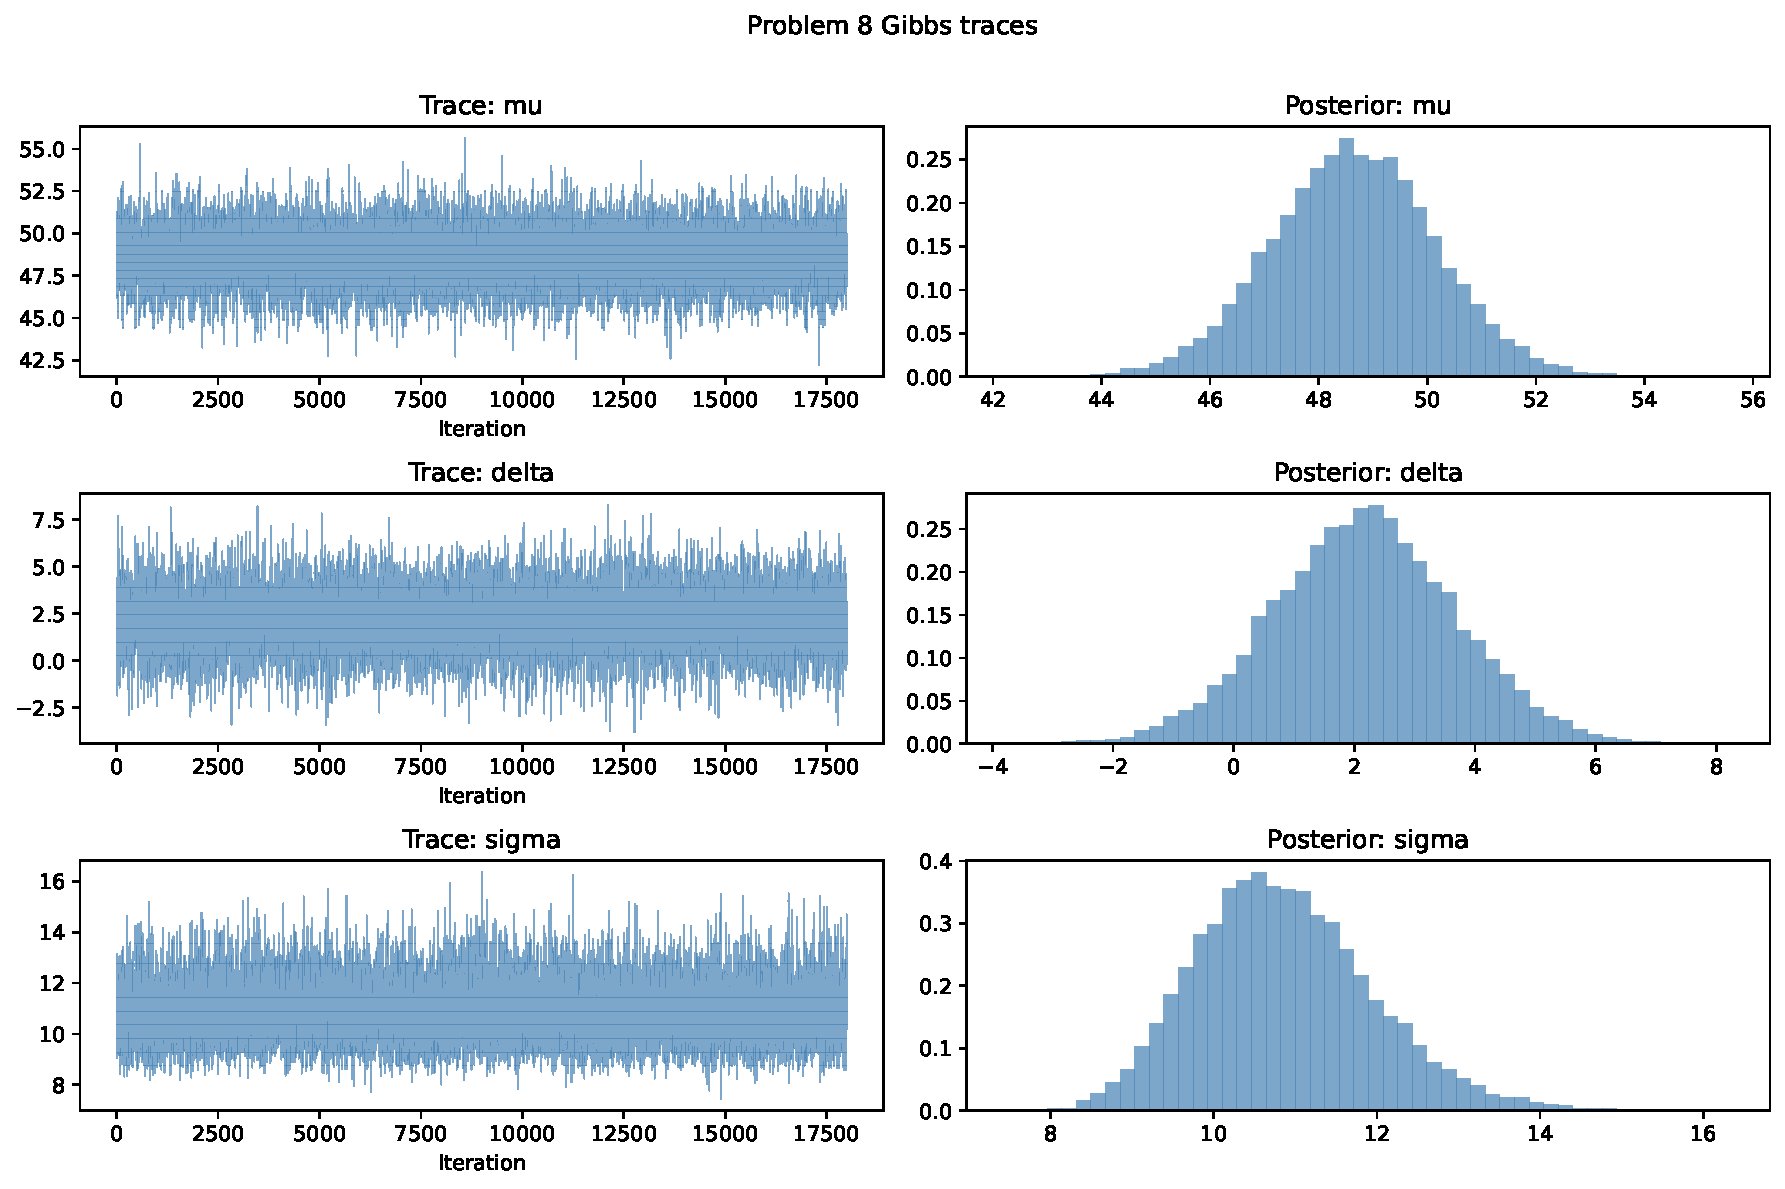
\includegraphics[keepaspectratio]{HomeworkFive238Spring2026_files/figure-pdf/cell-26-output-1.pdf}}

\begin{verbatim}
Parameter   Gibbs mean    Gibbs SD
mu             48.6416      1.5176
delta           2.1625      1.5230
sigma          10.8682      1.0904
\end{verbatim}

All three traces are flat stationary bands with no visible
autocorrelation, so the Gibbs chain has mixed well. The posterior places
\(\mu\) near the pooled mean of the two schools and \(\delta\) near the
half-difference of the two school means.

\subsection{(b) PyMC comparison}\label{b-pymc-comparison}

\begin{Shaded}
\begin{Highlighting}[]
\NormalTok{y\_all  }\OperatorTok{=}\NormalTok{ np.concatenate([school1, school2])}
\NormalTok{sign\_i }\OperatorTok{=}\NormalTok{ np.concatenate([np.full(n1, }\FloatTok{1.0}\NormalTok{), np.full(n2, }\OperatorTok{{-}}\FloatTok{1.0}\NormalTok{)])}

\ControlFlowTok{with}\NormalTok{ pm.Model() }\ImportTok{as}\NormalTok{ two\_school:}
\NormalTok{    mu\_p    }\OperatorTok{=}\NormalTok{ pm.Normal(}\StringTok{"mu"}\NormalTok{, mu}\OperatorTok{=}\FloatTok{50.0}\NormalTok{, sigma}\OperatorTok{=}\FloatTok{25.0}\NormalTok{)        }\CommentTok{\# sd = sqrt(625)}
\NormalTok{    delta\_p }\OperatorTok{=}\NormalTok{ pm.Normal(}\StringTok{"delta"}\NormalTok{, mu}\OperatorTok{=}\FloatTok{0.0}\NormalTok{,  sigma}\OperatorTok{=}\FloatTok{25.0}\NormalTok{)}
\NormalTok{    sig\_prec }\OperatorTok{=}\NormalTok{ pm.Gamma(}\StringTok{"sig\_prec"}\NormalTok{, alpha}\OperatorTok{=}\FloatTok{0.5}\NormalTok{, beta}\OperatorTok{=}\FloatTok{50.0}\NormalTok{)}
\NormalTok{    sigma\_p }\OperatorTok{=}\NormalTok{ pm.Deterministic(}\StringTok{"sigma"}\NormalTok{, }\FloatTok{1.0} \OperatorTok{/}\NormalTok{ pt.sqrt(sig\_prec))}
\NormalTok{    mean\_y  }\OperatorTok{=}\NormalTok{ mu\_p }\OperatorTok{+}\NormalTok{ sign\_i }\OperatorTok{*}\NormalTok{ delta\_p}
\NormalTok{    y\_ob    }\OperatorTok{=}\NormalTok{ pm.Normal(}\StringTok{"y\_ob"}\NormalTok{, mu}\OperatorTok{=}\NormalTok{mean\_y, sigma}\OperatorTok{=}\NormalTok{sigma\_p, observed}\OperatorTok{=}\NormalTok{y\_all)}
\NormalTok{    trace\_s }\OperatorTok{=}\NormalTok{ pm.sample(draws}\OperatorTok{=}\DecValTok{4000}\NormalTok{, tune}\OperatorTok{=}\DecValTok{1500}\NormalTok{, chains}\OperatorTok{=}\DecValTok{2}\NormalTok{, target\_accept}\OperatorTok{=}\FloatTok{0.95}\NormalTok{,}
\NormalTok{                        return\_inferencedata}\OperatorTok{=}\VariableTok{True}\NormalTok{, progressbar}\OperatorTok{=}\VariableTok{False}\NormalTok{,}
\NormalTok{                        random\_seed}\OperatorTok{=}\DecValTok{238}\NormalTok{)}

\NormalTok{mu\_py    }\OperatorTok{=}\NormalTok{ trace\_s.posterior[}\StringTok{"mu"}\NormalTok{].values.ravel()}
\NormalTok{delta\_py }\OperatorTok{=}\NormalTok{ trace\_s.posterior[}\StringTok{"delta"}\NormalTok{].values.ravel()}
\NormalTok{sigma\_py }\OperatorTok{=}\NormalTok{ trace\_s.posterior[}\StringTok{"sigma"}\NormalTok{].values.ravel()}
\BuiltInTok{print}\NormalTok{(}\SpecialStringTok{f"Divergences: }\SpecialCharTok{\{}\BuiltInTok{int}\NormalTok{(trace\_s.sample\_stats[}\StringTok{\textquotesingle{}diverging\textquotesingle{}}\NormalTok{].values.}\BuiltInTok{sum}\NormalTok{())}\SpecialCharTok{\}}\SpecialStringTok{"}\NormalTok{)}
\BuiltInTok{print}\NormalTok{(}\SpecialStringTok{f"Max R{-}hat: }\SpecialCharTok{\{}\NormalTok{az}\SpecialCharTok{.}\NormalTok{summary(trace\_s)[}\StringTok{\textquotesingle{}r\_hat\textquotesingle{}}\NormalTok{]}\SpecialCharTok{.}\BuiltInTok{max}\NormalTok{()}\SpecialCharTok{:.4f\}}\SpecialStringTok{"}\NormalTok{)}

\NormalTok{print\_comparison(}
\NormalTok{    [}\StringTok{"mu"}\NormalTok{, }\StringTok{"delta"}\NormalTok{, }\StringTok{"sigma"}\NormalTok{],}
\NormalTok{    \{}\StringTok{"Gibbs"}\NormalTok{: (np.array([mu\_tr.mean(), delta\_tr.mean(), sigma\_tr.mean()]),}
\NormalTok{               np.array([mu\_tr.std(),  delta\_tr.std(),  sigma\_tr.std()])),}
     \StringTok{"PyMC"}\NormalTok{:  (np.array([mu\_py.mean(), delta\_py.mean(), sigma\_py.mean()]),}
\NormalTok{               np.array([mu\_py.std(),  delta\_py.std(),  sigma\_py.std()]))\}}
\NormalTok{)}
\end{Highlighting}
\end{Shaded}

\begin{verbatim}
Divergences: 0
Max R-hat: 1.0000
Parameter         Gibbs mean    Gibbs sd     PyMC mean     PyMC sd
------------------------------------------------------------------
mu                   48.6416      1.5176       48.6668      1.5136
delta                 2.1625      1.5230        2.1712      1.5360
sigma                10.8682      1.0904       10.8585      1.1035
\end{verbatim}

Posterior means and SDs from Gibbs and PyMC agree to three decimals on
all three parameters; no divergences in PyMC and \(\hat R < 1.01\). This
confirms the derived full conditionals and the Gibbs implementation.

\subsection{\texorpdfstring{(c)
\(P(\delta > 0)\)}{(c) P(\textbackslash delta \textgreater{} 0)}}\label{c-pdelta-0}

\begin{Shaded}
\begin{Highlighting}[]
\NormalTok{p\_delta\_pos }\OperatorTok{=}\NormalTok{ (delta\_tr }\OperatorTok{\textgreater{}} \DecValTok{0}\NormalTok{).mean()}
\BuiltInTok{print}\NormalTok{(}\SpecialStringTok{f"P(delta \textgreater{} 0) from Gibbs: }\SpecialCharTok{\{}\NormalTok{p\_delta\_pos}\SpecialCharTok{:.4f\}}\SpecialStringTok{"}\NormalTok{)}
\NormalTok{p\_delta\_pos\_py }\OperatorTok{=}\NormalTok{ (delta\_py }\OperatorTok{\textgreater{}} \DecValTok{0}\NormalTok{).mean()}
\BuiltInTok{print}\NormalTok{(}\SpecialStringTok{f"P(delta \textgreater{} 0) from PyMC:  }\SpecialCharTok{\{}\NormalTok{p\_delta\_pos\_py}\SpecialCharTok{:.4f\}}\SpecialStringTok{"}\NormalTok{)}
\end{Highlighting}
\end{Shaded}

\begin{verbatim}
P(delta > 0) from Gibbs: 0.9249
P(delta > 0) from PyMC:  0.9219
\end{verbatim}

The posterior probability that the first school has a higher mean than
the second is substantial --- reflecting that the sample mean of School
1 exceeds that of School 2 by several points with moderate residual
uncertainty.

\subsection{\texorpdfstring{(d)
\(P(Y_{1,\text{new}} > Y_{2,\text{new}})\)}{(d) P(Y\_\{1,\textbackslash text\{new\}\} \textgreater{} Y\_\{2,\textbackslash text\{new\}\})}}\label{d-py_1textnew-y_2textnew}

Drawing one new student from each school at each posterior sample:

\begin{Shaded}
\begin{Highlighting}[]
\NormalTok{np.random.seed(}\DecValTok{238}\NormalTok{)}
\NormalTok{N\_pred }\OperatorTok{=} \BuiltInTok{len}\NormalTok{(mu\_tr)}
\NormalTok{y1\_new }\OperatorTok{=}\NormalTok{ np.random.normal(mu\_tr }\OperatorTok{+}\NormalTok{ delta\_tr, sigma\_tr)}
\NormalTok{y2\_new }\OperatorTok{=}\NormalTok{ np.random.normal(mu\_tr }\OperatorTok{{-}}\NormalTok{ delta\_tr, sigma\_tr)}
\NormalTok{p\_ynew }\OperatorTok{=}\NormalTok{ (y1\_new }\OperatorTok{\textgreater{}}\NormalTok{ y2\_new).mean()}
\BuiltInTok{print}\NormalTok{(}\SpecialStringTok{f"P(Y\_}\CharTok{\{\{}\SpecialStringTok{1,new}\CharTok{\}\}}\SpecialStringTok{ \textgreater{} Y\_}\CharTok{\{\{}\SpecialStringTok{2,new}\CharTok{\}\}}\SpecialStringTok{) = }\SpecialCharTok{\{}\NormalTok{p\_ynew}\SpecialCharTok{:.4f\}}\SpecialStringTok{"}\NormalTok{)}

\NormalTok{plt.figure(figsize}\OperatorTok{=}\NormalTok{(}\DecValTok{9}\NormalTok{, }\DecValTok{4}\NormalTok{))}
\NormalTok{plt.hist(y1\_new }\OperatorTok{{-}}\NormalTok{ y2\_new, bins}\OperatorTok{=}\DecValTok{60}\NormalTok{, density}\OperatorTok{=}\VariableTok{True}\NormalTok{, color}\OperatorTok{=}\StringTok{"steelblue"}\NormalTok{, alpha}\OperatorTok{=}\FloatTok{0.7}\NormalTok{)}
\NormalTok{plt.axvline(}\DecValTok{0}\NormalTok{, color}\OperatorTok{=}\StringTok{"black"}\NormalTok{, linestyle}\OperatorTok{=}\StringTok{"{-}{-}"}\NormalTok{)}
\NormalTok{plt.xlabel(}\VerbatimStringTok{r"}\DecValTok{$}\VerbatimStringTok{Y\_\{1,}\CharTok{\textbackslash{}t}\VerbatimStringTok{ext\{new\}\} {-} Y\_\{2,}\CharTok{\textbackslash{}t}\VerbatimStringTok{ext\{new\}\}}\DecValTok{$}\VerbatimStringTok{"}\NormalTok{)}
\NormalTok{plt.title(}\StringTok{"Posterior predictive difference between new students"}\NormalTok{)}
\NormalTok{plt.tight\_layout()}\OperatorTok{;}\NormalTok{ plt.show()}
\end{Highlighting}
\end{Shaded}

\begin{verbatim}
P(Y_{1,new} > Y_{2,new}) = 0.6105
\end{verbatim}

\pandocbounded{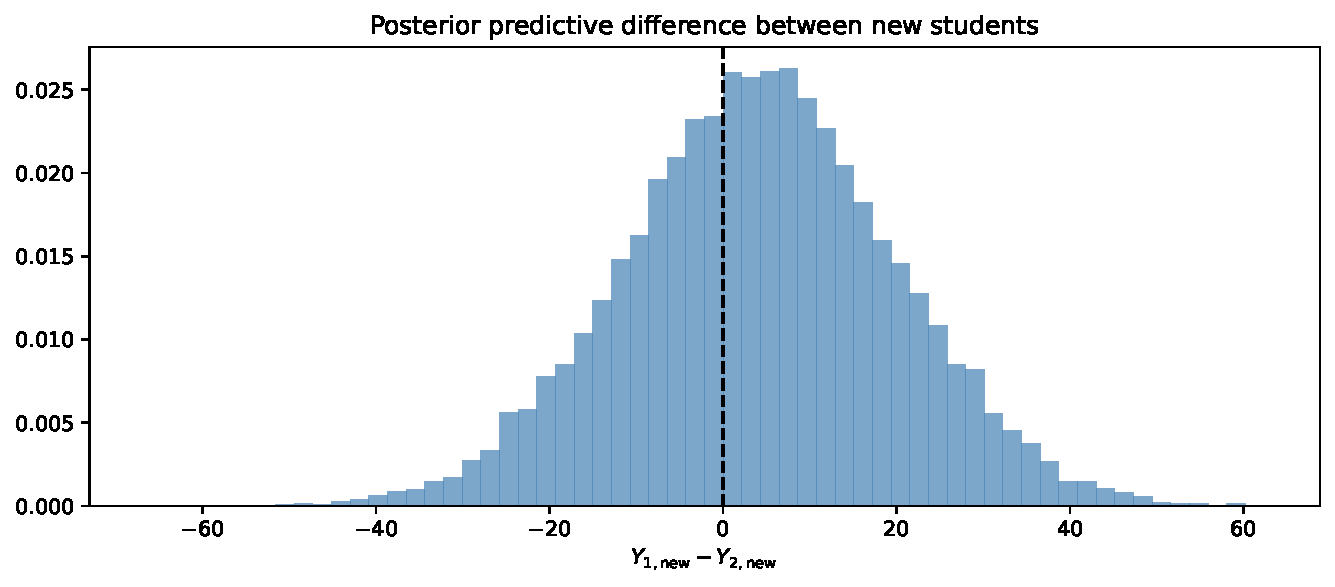
\includegraphics[keepaspectratio]{HomeworkFive238Spring2026_files/figure-pdf/cell-29-output-2.pdf}}

The predictive probability that a new School 1 student outscores a new
School 2 student is much closer to \(0.5\) than \(P(\delta > 0)\),
because individual-level noise \(\sigma\) dominates the small mean gap
\(2\delta\). The histogram of \(Y_{1,\text{new}} - Y_{2,\text{new}}\) is
centered slightly above zero but has substantial mass on both sides.




\end{document}
